%% Author: Saleem Al Dajani, MIT, KAUST. UCB-NE
%DIF LATEXDIFF DIFFERENCE FILE
%DIF DEL finalpaper_mike_reviewed.tex   Mon Oct 12 06:12:19 2026
%DIF ADD finalpaper.tex                 Mon Oct 12 17:54:52 2026
%% This is the manuscript draft for our paper about LWR MMLC
% draft format
%\documentclass[preprint,12pt]{elsarticle}

% final submission format
%\documentclass[preprint, review, 12pt]{elsarticle}

%% Use the option review to obtain double line spacing
%% \documentclass[preprint,review,12pt]{elsarticle}

%% Use the options 1p,twocolumn; 3p; 3p,twocolumn; 5p; or 5p,twocolumn
%% for a journal layout:
%% \documentclass[final,1p,times]{elsarticle}
%% \documentclass[final,1p,times,twocolumn]{elsarticle}
\PassOptionsToPackage{numbers,sort&compress}{natbib}
\documentclass[final,3p,times]{elsarticle}
%\documentclass[final,3p,times,twocolumn]{elsarticle}
%% \documentclass[final,5p,times]{elsarticle}
%% \documentclass[final,5p,times,twocolumn]{elsarticle}
\usepackage{natbib}
%% The graphicx package provides the includegraphics command.
\usepackage{graphicx}
%% The amssymb package provides various useful mathematical symbols
\usepackage{amssymb}
\usepackage{amsmath} 
%% The amsthm package provides extended theorem environments
%% \usepackage{amsthm}
\usepackage{fancyhdr}
\usepackage{hyperref}
\usepackage{caption}
\usepackage{subcaption}
\usepackage{wrapfig}
\usepackage{lscape}
\usepackage{rotating}
\usepackage{epstopdf}
\usepackage{comment}
\usepackage{xurl}
%\usepackage[figuresfirst,nomarkers,nolists,figuresonly,noheads]{endfloat}
% Tell endfloat to handle sidewaysfigure the same as figure
%\DeclareDelayedFloatFlavor{sidewaysfigure}{figure}
\makeatletter
\def\NAT@def@citea{\def\@citea{\NAT@separator}}
\makeatother
\hypersetup{
colorlinks,
citecolor=blue,
filecolor=blue,
linkcolor=blue,
urlcolor=blue
}

%% The lineno packages adds line numbers. Start line numbering with
%% \begin{linenumbers}, end it with \end{linenumbers}. Or switch it on
%% for the whole article with \linenumbers after \end{frontmatter}.
\usepackage{lineno}

%% natbib.sty is loaded by default. However, natbib options can be
%% provided with \biboptions{...} command. Following options are
%% valid:

%%   round  -  round parentheses are used (default)
%%   square -  square brackets are used   [option]
%%   curly  -  curly braces are used      {option}
%%   angle  -  angle brackets are used    <option>
%%   semicolon  -  multiple citations separated by semi-colon
%%   colon  - same as semicolon, an earlier confusion
%%   comma  -  separated by comma
%%   numbers-  selects numerical citations
%%   super  -  numerical citations as superscripts
%%   sort   -  sorts multiple citations according to order in ref. list
%%   sort&compress   -  like sort, but also compresses numerical citations
%%   compress - compresses without sorting
%%
%% \biboptions{comma,round}

% \biboptions{}

%DIF 79a79-81
\usepackage{xcolor} %DIF > 
\usepackage{booktabs} %DIF > 
 %DIF > 
%DIF -------
\journal{Scripta Materialia}
%DIF PREAMBLE EXTENSION ADDED BY LATEXDIFF
%DIF UNDERLINE PREAMBLE %DIF PREAMBLE
\RequirePackage[normalem]{ulem} %DIF PREAMBLE
\RequirePackage{color}\definecolor{RED}{rgb}{1,0,0}\definecolor{BLUE}{rgb}{0,0,1} %DIF PREAMBLE
\providecommand{\DIFaddtex}[1]{{\protect\color{blue}\uwave{#1}}} %DIF PREAMBLE
\providecommand{\DIFdeltex}[1]{{\protect\color{red}\sout{#1}}} %DIF PREAMBLE
%DIF SAFE PREAMBLE %DIF PREAMBLE
\providecommand{\DIFaddbegin}{} %DIF PREAMBLE
\providecommand{\DIFaddend}{} %DIF PREAMBLE
\providecommand{\DIFdelbegin}{} %DIF PREAMBLE
\providecommand{\DIFdelend}{} %DIF PREAMBLE
\providecommand{\DIFmodbegin}{} %DIF PREAMBLE
\providecommand{\DIFmodend}{} %DIF PREAMBLE
%DIF FLOATSAFE PREAMBLE %DIF PREAMBLE
\providecommand{\DIFaddFL}[1]{\DIFadd{#1}} %DIF PREAMBLE
\providecommand{\DIFdelFL}[1]{\DIFdel{#1}} %DIF PREAMBLE
\providecommand{\DIFaddbeginFL}{} %DIF PREAMBLE
\providecommand{\DIFaddendFL}{} %DIF PREAMBLE
\providecommand{\DIFdelbeginFL}{} %DIF PREAMBLE
\providecommand{\DIFdelendFL}{} %DIF PREAMBLE
%DIF HYPERREF PREAMBLE %DIF PREAMBLE
\providecommand{\DIFadd}[1]{\texorpdfstring{\DIFaddtex{#1}}{#1}} %DIF PREAMBLE
\providecommand{\DIFdel}[1]{\texorpdfstring{\DIFdeltex{#1}}{}} %DIF PREAMBLE
\providecommand{\DIFscaledelfig}{0.5}
%DIF HIGHLIGHTGRAPHICS PREAMBLE %DIF PREAMBLE
\RequirePackage{settobox} %DIF PREAMBLE
\RequirePackage{letltxmacro} %DIF PREAMBLE
\newsavebox{\DIFdelgraphicsbox} %DIF PREAMBLE
\newlength{\DIFdelgraphicswidth} %DIF PREAMBLE
\newlength{\DIFdelgraphicsheight} %DIF PREAMBLE
% store original definition of \includegraphics %DIF PREAMBLE
\LetLtxMacro{\DIFOincludegraphics}{\includegraphics} %DIF PREAMBLE
\providecommand{\DIFaddincludegraphics}[2][]{{\color{blue}\fbox{\DIFOincludegraphics[#1]{#2}}}} %DIF PREAMBLE
\providecommand{\DIFdelincludegraphics}[2][]{% %DIF PREAMBLE
\sbox{\DIFdelgraphicsbox}{\DIFOincludegraphics[#1]{#2}}% %DIF PREAMBLE
\settoboxwidth{\DIFdelgraphicswidth}{\DIFdelgraphicsbox} %DIF PREAMBLE
\settoboxtotalheight{\DIFdelgraphicsheight}{\DIFdelgraphicsbox} %DIF PREAMBLE
\scalebox{\DIFscaledelfig}{% %DIF PREAMBLE
\parbox[b]{\DIFdelgraphicswidth}{\usebox{\DIFdelgraphicsbox}\\[-\baselineskip] \rule{\DIFdelgraphicswidth}{0em}}\llap{\resizebox{\DIFdelgraphicswidth}{\DIFdelgraphicsheight}{% %DIF PREAMBLE
\setlength{\unitlength}{\DIFdelgraphicswidth}% %DIF PREAMBLE
\begin{picture}(1,1)% %DIF PREAMBLE
\thicklines\linethickness{2pt} %DIF PREAMBLE
{\color[rgb]{1,0,0}\put(0,0){\framebox(1,1){}}}% %DIF PREAMBLE
{\color[rgb]{1,0,0}\put(0,0){\line( 1,1){1}}}% %DIF PREAMBLE
{\color[rgb]{1,0,0}\put(0,1){\line(1,-1){1}}}% %DIF PREAMBLE
\end{picture}% %DIF PREAMBLE
}\hspace*{3pt}}} %DIF PREAMBLE
} %DIF PREAMBLE
\LetLtxMacro{\DIFOaddbegin}{\DIFaddbegin} %DIF PREAMBLE
\LetLtxMacro{\DIFOaddend}{\DIFaddend} %DIF PREAMBLE
\LetLtxMacro{\DIFOdelbegin}{\DIFdelbegin} %DIF PREAMBLE
\LetLtxMacro{\DIFOdelend}{\DIFdelend} %DIF PREAMBLE
\DeclareRobustCommand{\DIFaddbegin}{\DIFOaddbegin \let\includegraphics\DIFaddincludegraphics} %DIF PREAMBLE
\DeclareRobustCommand{\DIFaddend}{\DIFOaddend \let\includegraphics\DIFOincludegraphics} %DIF PREAMBLE
\DeclareRobustCommand{\DIFdelbegin}{\DIFOdelbegin \let\includegraphics\DIFdelincludegraphics} %DIF PREAMBLE
\DeclareRobustCommand{\DIFdelend}{\DIFOaddend \let\includegraphics\DIFOincludegraphics} %DIF PREAMBLE
\LetLtxMacro{\DIFOaddbeginFL}{\DIFaddbeginFL} %DIF PREAMBLE
\LetLtxMacro{\DIFOaddendFL}{\DIFaddendFL} %DIF PREAMBLE
\LetLtxMacro{\DIFOdelbeginFL}{\DIFdelbeginFL} %DIF PREAMBLE
\LetLtxMacro{\DIFOdelendFL}{\DIFdelendFL} %DIF PREAMBLE
\DeclareRobustCommand{\DIFaddbeginFL}{\DIFOaddbeginFL \let\includegraphics\DIFaddincludegraphics} %DIF PREAMBLE
\DeclareRobustCommand{\DIFaddendFL}{\DIFOaddendFL \let\includegraphics\DIFOincludegraphics} %DIF PREAMBLE
\DeclareRobustCommand{\DIFdelbeginFL}{\DIFOdelbeginFL \let\includegraphics\DIFdelincludegraphics} %DIF PREAMBLE
\DeclareRobustCommand{\DIFdelendFL}{\DIFOaddendFL \let\includegraphics\DIFOincludegraphics} %DIF PREAMBLE
%DIF AMSMATHULEM PREAMBLE %DIF PREAMBLE
\makeatletter %DIF PREAMBLE
\let\sout@orig\sout %DIF PREAMBLE
\renewcommand{\sout}[1]{\ifmmode\text{\sout@orig{\ensuremath{#1}}}\else\sout@orig{#1}\fi} %DIF PREAMBLE
\makeatother %DIF PREAMBLE
%DIF END PREAMBLE EXTENSION ADDED BY LATEXDIFF

\begin{document}
\begin{frontmatter}

%DIF < % Title, authors and addresses
\DIFdelbegin %DIFDELCMD < 

%DIFDELCMD < %%%
\DIFdelend \title
{
\textbf
{
First principles evidence of stiffening \\ during spinodal decomposition in FeCr
}
}

\date
{\today}
\rhead{\today}
%DIF < % use the tnoteref command within \title for footnotes;
%DIF < % use the tnotetext command for the associated footnote;
%DIF < % use the fnref command within \author or \address for footnotes;
%DIF < % use the fntext command for the associated footnote;
%DIF < % use the corref command within \author for corresponding author footnotes;
%DIF < % use the cortext command for the associated footnote;
%DIF < % use the ead command for the email address,
%DIF < % and the form \ead[url] for the home page:
%DIF < %
%DIF < % \title{Title\tnoteref{label1}}
%DIF < % \tnotetext[label1]{}
%DIF < % \author{Name\corref{cor1}\fnref{label2}}
%DIF < % \ead{email address}
%DIF < % \ead[url]{home page}
%DIF < % \fntext[label2]{}
%DIF < % \cortext[cor1]{}
%DIF < % \address{Address\fnref{label3}}
%DIF < % \fntext[label3]{}

%DIF < % use optional labels to link authors explicitly to addresses:
%DIF < % \author[label1,label2]{<author name>}
%DIF < % \address[label1]{<address>}
%DIF < % \address[label2]{<address>}
\DIFdelbegin %DIFDELCMD < 

%DIFDELCMD < %%%
\DIFdelend \author[1]{Saleem A. Al Dajani}
%DIF < \author{Ben R. Dacus}
%DIF < \author{Cody A. Dennett}
%DIF < \author{Samuel W. McAlpine}
%DIF < \author{Peter Hosemann}
%DIF < \author{Udo Schwingenschlogl}
\author[1]{Michael P. Short}

\address{
Department of Nuclear Science and Engineering \\
Massachusetts Institute of Technology\\
77 Massachusetts Avenue \\
Cambridge, MA 02139}

\address[1]
{
Corresponding Author: \href{mailto:sdajani@mit.edu}{\texttt{sdajani@mit.edu}}
}
%DIF < \address[2]{\texttt{hereiam@mit.edu}}
\DIFaddbegin 

\DIFaddend \begin{abstract}

We explain stiffening during spinodal decomposition in \emph{bcc} $\delta$-ferrite previously observed in cast austenitic stainless steels by combining experimental measurements with first-principles simulations of \emph{bcc} Fe$_{1-x}$Cr$_x$. Quantum elastodynamic calculations predict surface acoustic wave (SAW) peak splitting arising from elastic stiffening of $\delta$-ferrite during spinodal decomposition. Classical first-principles elastodynamics also quantitatively calculate Rayleigh SAW peak splitting arising from spinodal stiffening as a non-destructive indicator of embrittlement, in agreement with experiment\DIFdelbegin \DIFdel{and beyond what classical molecular dynamics captures without electronic structure}\DIFdelend . More broadly, \DIFdelbegin \DIFdel{the same }\DIFdelend \DIFaddbegin \DIFadd{similar }\DIFaddend SAW-based stiffening \DIFdelbegin \DIFdel{signature may extend to }\DIFdelend \DIFaddbegin \DIFadd{signatures may prove useful for detecting }\DIFaddend other embrittlement mechanisms in structural alloys\DIFdelbegin \DIFdel{, such as Cu precipitation in reactor pressure vessel (RPV) steels}\DIFdelend .

\end{abstract}

\begin{keyword}
Stainless steel \sep 
binary alloy \sep
iron-chrome \sep
spinodal decomposition
\sep
surface acoustic wave \sep 
\emph{Ab initio} calculation
\sep
stiffening
\sep
embrittlement
\sep
thermal diffusivity
\sep
$\delta$--ferrite
\sep
quantum elastodynamics (QED)
%% keywords here, in the form: keyword \sep keyword

%% MSC codes here, in the form: \MSC code \sep code
%% or \MSC[2008] code \sep code (2000 is the default)

\end{keyword}

\end{frontmatter}

\textbf{Highlights}

\begin{itemize}
\item \DIFdelbegin \DIFdel{Spinodal decomposition in bcc }\DIFdelend \DIFaddbegin \DIFadd{Ab initio simulations predict stiffening during spinodal decomposition in }\DIFaddend $\delta$--ferrite
\DIFdelbegin \DIFdel{induces stiffening captured by }\emph{\DIFdel{ab initio}} %DIFAUXCMD
\DIFdel{quantum elastodynamics
}\DIFdelend \item Composition-dependent elasticity maps to \DIFdelbegin \DIFdel{Rayleigh }\DIFdelend surface acoustic wave frequency shifts
\DIFdelbegin \DIFdel{and peak splitting
}\DIFdelend \item \DIFdelbegin \DIFdel{Theoretical and experimental agreement demonstrates stiffening as a non-destructive indicator of }\DIFdelend \DIFaddbegin \DIFadd{Theory and experiment agree: stiffening non-destructively indicates }\DIFaddend embrittlement
\end{itemize}


\section{Introduction and Background}
Recent structure--property studies have linked spinodal decomposition to stiffening of \textit{bcc} $\delta$--ferrite in cast austenitic stainless steels (CASS), and have shown that this stiffening can be detected through picosecond ultrasonic surface acoustic wave (SAW) peak splitting \cite{al2023detecting, al2020detecting,al2020non}.
This paper establishes a quantitative theoretical foundation for predicting that SAW signature from first principles by combining elastodynamics with density functional theory (DFT) to connect composition, elastic response, and Rayleigh-wave observables.

For high--melting-point metals (including \textit{bcc} $\delta$--ferrite), elasticity is often closely tied to plastic response: dislocation energetics are largely stored in the Hookean lattice outside the dislocation core, and thermally activated processes during deformation can modify elastic properties \cite{pugh1954xcii}.
More broadly, cohesive properties quantified by lattice elasticity correlate with melting point through their shared dependence on interatomic bonding and electronic structure \cite{chang1966correlation,fine1984elastic, korzhavyi2009electronic, razumovskiy2011first, hosemann2018materials}.
In ferromagnetic Fe--Cr alloys, these quantities vary strongly with concentration \cite{korzhavyi2009electronic}, and the experimentally observed SAW peak splitting upon spinodal decomposition is consistent with an anomalous concentration dependence of elastic constants associated with electronic-structure effects (including Fermi-surface topology changes \cite{razumovskiy2011first}).

During spinodal decomposition of \textit{bcc} $\delta$--ferrite, chromium partitioning produces Fe-rich $\alpha$ and Cr-rich $\alpha'$ regions whose differing compositions imply differing stiffness. As a result, elastic stiffening can serve as a mechanistically grounded proxy for embrittlement in stainless steels undergoing thermal and/or irradiation-assisted aging \cite{du2017facile, sdajani2019cassspinodal,al2020non, hofmann2019transient, al2020detecting,byun2016thermal,lach2020precipitation}.
Because the Rayleigh SAW frequency depends directly on elastic moduli, picosecond ultrasonic pump--probe spectroscopy provides a direct, non-destructive route to infer stiffness changes and therefore track the progression toward embrittlement \cite{hofmann2019transient}.

Motivated by these links, we develop a thermodynamics-to-observable workflow for \textit{bcc} Fe$_{1-x}$Cr$_x$ as a model for $\delta$--ferrite: (i) we identify spinodally unstable composition windows using the curvature of the demixing free energy, (ii) we quantify the composition dependence of cubic elastic constants from DFT, and (iii) we map these elastic inputs into Rayleigh SAW frequency ranges using elastodynamic constraints relevant to picosecond ultrasonics. Finally, we separate a solid-solution trend $f_{\mathrm{SAW}}(x_{\mathrm{Cr}})$ from an evolution trend $f_{\mathrm{SAW}}(\phi)$ parameterized by the spinodal conversion fraction $\phi$ from \DIFdelbegin \DIFdel{molecular dynamics (MD)}\DIFdelend \DIFaddbegin \DIFadd{our earlier atomistic simulations of decomposed Fe--Cr \mbox{%DIFAUXCMD
\cite{al2023detecting}}\hskip0pt%DIFAUXCMD
}\DIFaddend , enabling direct interpretation of SAW peak shifts and splitting in terms of composition and decomposition state.


\section{Methods}

%DIF < \subsection{TGS Methods}
%DIF <  Include specific details about TGS methods here.
\DIFdelbegin %DIFDELCMD < 

%DIFDELCMD < %%%
\DIFdelend \subsection{Elastodynamic Methods}
\DIFdelbegin \DIFdel{In this work, materials are modeled as anisotropic unbounded media through which elastic waves propagate according to }\DIFdelend \DIFaddbegin \DIFadd{Elastic waves in each homogeneous alloy obey }\DIFaddend the elastodynamic wave equation \cite{du2017facile}:

\begin{equation}
    \DIFaddbegin \DIFadd{\rho \frac{\partial^2 u_i}{\partial t^2} = }\DIFaddend C_{ijkl} \DIFdelbegin \DIFdel{\frac{\partial U_l(\vec{r},t)}{\partial x_j\partial x_k}= \rho(}%DIFDELCMD < \vec{r}%%%
\DIFdel{,t)\frac{\partial^2 U_l(\vec{r},t)}{\partial t^2}
    }\DIFdelend \DIFaddbegin \DIFadd{\frac{\partial^2 u_k}{\partial x_j \partial x_l}
    }\DIFaddend \label{eqn:ewe}
\end{equation}

where $C_{ijkl}$ are fourth-order stiffness tensor entries \DIFdelbegin \DIFdel{that are permutatively }\DIFdelend indexed by $i,j,k,l=1,2,3$, $\rho$ is density, and \DIFdelbegin \DIFdel{$U$ is the wave function. }\DIFdelend \DIFaddbegin \DIFadd{$u$ is the displacement field. On its own, Eq.~\ref{eqn:ewe} describes bulk waves in an unbounded medium. The SAW measured by transient grating spectroscopy (TGS), however, is a Rayleigh wave guided by the free surface. It is obtained from Eq.~\ref{eqn:ewe} for a half-space $x_3 \geq 0$ by requiring a traction-free surface, $\sigma_{i3} = C_{i3kl}\,\partial u_k/\partial x_l = 0$ at $x_3=0$, and displacements that decay with depth. Because crystal orientation is not resolved in the present calculations, we solve this surface problem for the isotropic Voigt--Reuss--Hill (VRH) average of each elastic tensor (Sec.~\ref{sec:analysis}). The Rayleigh velocity is then $v_R = v_s\sqrt{q}$, where $q$ is the root in $0<q<1$ of
}\begin{equation}
\DIFadd{q^3 - 8q^2 + (24-16\beta)q - 16(1-\beta) = 0, \qquad \beta = v_s^2/v_p^2,
\label{eqn:rayleigh}
}\end{equation}
\DIFadd{with $v_s=\sqrt{G/\rho}=\sqrt{E/[2(1+\nu)\rho]}$ and $v_p=\sqrt{(B+4G/3)/\rho}$. In practice we evaluate $v_R=(0.874+0.196\nu-0.042\nu^2-0.055\nu^3)\,v_s$, which reproduces the root of Eq.~\ref{eqn:rayleigh} to within 0.02\% for $0.20\leq\nu\leq0.35$. The SAW frequency is $f_{\mathrm{SAW}} = v_R/\lambda$ with $\lambda = 6.4\,\mu$m, the grating period of our TGS measurements \mbox{%DIFAUXCMD
\cite{al2023detecting}}\hskip0pt%DIFAUXCMD
. Density is interpolated linearly between }\textit{\DIFadd{bcc}} \DIFadd{Fe (7870 kg m$^{-3}$) and Cr (7200 kg m$^{-3}$).
}\DIFaddend 

The elastic tensor is calculated using a variable cell relaxation algorithm that consists of a loop over iterative \DIFdelbegin \DIFdel{SCF }\DIFdelend \DIFaddbegin \DIFadd{self-consistent field (SCF) }\DIFaddend calculations while adjusting atomic positions and lattice constants. Elasticity theory relates the strain applied to the unit cell to the resulting calculated stress as an inverse problem, which could be solved using a non-linear solver with prior data as an initial guess vector. Deterministic thermoelastic relationships are also used to calculate elastic tensors from changes in total energy and volume using \textit{ab initio} stress calculations. Both methods are used in a self-consistent fashion to converge to a solution that solves the elasticity inverse problem, $\underline{C}\vec{\epsilon} = \vec{\sigma}$, as follows \cite{timoshenko1951theory, mit1620}:

\begin{equation} \label{eqn:stiffness-full-notation}
\begin{bmatrix}
C_{1111} & C_{1122} & C_{1133} & C_{1123} & C_{1113} & C_{1112} \\
 & C_{2222} & C_{2233} & C_{2223} & C_{2213} & C_{2212} \\
 &  & C_{3333} & C_{3323} & C_{3313} & C_{3312} \\
 &  &  & C_{2323} & C_{2313} & C_{2312} \\
 & symm &  &  & C_{1313} & C_{1312} \\
 &  &  &  &  & C_{1212}
\end{bmatrix} \begin{bmatrix}
\epsilon_{11} \\
\epsilon_{22} \\
\epsilon_{33} \\
2\epsilon_{23} \\
2\epsilon_{13} \\
2\epsilon_{12}
\end{bmatrix}  =  \begin{bmatrix}
\sigma_{11} \\
\sigma_{22} \\
\sigma_{33} \\
\sigma_{23} \\
\sigma_{13} \\
\sigma_{12}
\end{bmatrix}
\end{equation}
or in Voigt notation:
\begin{equation} \label{eqn:stiffness-voigt-notation}
 \begin{bmatrix}
C_{11} & C_{12} & C_{13} & C_{14} & C_{15} & C_{16} \\
 & C_{22} & C_{23} & C_{24} & C_{25} & C_{26} \\
 &  & C_{33} & C_{34} & C_{35} & C_{36} \\
 &  &  & C_{44} & C_{45} & C_{46} \\
 & symm &  &  & C_{55} & C_{56} \\
 &  &  &  &  & C_{66}
\end{bmatrix}  \begin{bmatrix}
\epsilon_{1} \\
\epsilon_{2} \\
\epsilon_{3} \\
\epsilon_{4} \\
\epsilon_{5} \\
\epsilon_{6}
\end{bmatrix}  =  \begin{bmatrix}
\sigma_{1} \\
\sigma_{2} \\
\sigma_{3} \\
\sigma_{4} \\
\sigma_{5} \\
\sigma_{6}
\end{bmatrix}
\end{equation}


\subsection{DFT Methods}
Material properties are calculated from a self-consistent, non-linear field calculation \DIFdelbegin \DIFdel{, }\DIFdelend (Fig.\DIFdelbegin \DIFdel{\ref{fig:SCF-loop}) which is }\DIFdelend \DIFaddbegin \DIFadd{~\ref{fig:SCF-loop}), }\DIFaddend a variational method that optimizes \DIFdelbegin \DIFdel{over charge density that }\DIFdelend \DIFaddbegin \DIFadd{the charge density and }\DIFaddend adjusts atomic positions until a threshold in energy minimization is achieved in a simplified ion-core model of atoms and electrons \DIFdelbegin \DIFdel{in a given material to solve the many-body wave equation \mbox{%DIFAUXCMD
\cite{Schwingenschloegl2004}}\hskip0pt%DIFAUXCMD
.
Electron dispersion is calculated using a non-consistent field calculation to interpolate the energy calculations in momentum space. The phonon dispersion is calculated from the dynamical matrix obtained from }\textit{\DIFdel{ab initio}} %DIFAUXCMD
\DIFdel{calculations \mbox{%DIFAUXCMD
\cite{hung2022quantum, giustino2014materials}}\hskip0pt%DIFAUXCMD
.
}\DIFdelend \DIFaddbegin \DIFadd{\mbox{%DIFAUXCMD
\cite{Schwingenschloegl2004}}\hskip0pt%DIFAUXCMD
.
}\DIFaddend 

Self-consistent, non-linear field calculation algorithms calculate external potentials with a Poisson equation solver, (Fig.\DIFaddbegin \DIFadd{~}\DIFaddend \ref{fig:SCF-loop}) which depends on simulation geometry, atomic positions of ions, pseudopotentials used for the atoms involved, and other inputs. This external potential is then used as a guess for the electron density with a Schr\"{o}dinger equation solver \cite{giustino2014materials}, which is then used as inputs to a self-consistent field loop that calculates the charge density iteratively to minimize the total energy. The accuracy of this algorithm depends on the cut-off applied to the energy minimization, the charge density, the size of the momentum grid, and other convergence thresholds on the outputs \cite{hung2022quantum, Schwingenschloegl2004, giustino2014materials}.

In order to model the BCC Fe--Cr $\delta$--ferrite solid solution, the \DIFdelbegin \DIFdel{sequential }\DIFdelend \DIFaddbegin \DIFadd{special }\DIFaddend quasirandom structure (SQS) methodology was employed \cite{VandeWalleLiu2013}.
The \texttt{mcsqs} software package within the Alloy Theoretic Automated Toolkit (ATAT) was used in order to generate SQS supercells.
The Vienna \textit{ab initio} Simulation Package (VASP) \DIFaddbegin \DIFadd{\mbox{%DIFAUXCMD
\cite{kresse1996vasp} }\hskip0pt%DIFAUXCMD
}\DIFaddend was used to perform the density functional theory (DFT) total energy calculations, which were used to derive the elastic properties as well as the enthalpy of mixing.
Spin--polarized DFT calculations were performed on 40--atom SQS supercells employing $\Gamma$--point sampling of reciprocal space along with a 500 eV planewave cutoff energy.
The Projector--Augmented Wave (PAW) method \DIFaddbegin \DIFadd{\mbox{%DIFAUXCMD
\cite{kresse1999paw} }\hskip0pt%DIFAUXCMD
}\DIFaddend was employed for the ionic pseudopotential, and the \DIFdelbegin \DIFdel{Perdew--Burke--Ernzenhoffer parameterization }\DIFdelend \DIFaddbegin \DIFadd{Perdew--Burke--Ernzerhof parameterization \mbox{%DIFAUXCMD
\cite{pbe1996} }\hskip0pt%DIFAUXCMD
}\DIFaddend of the Generalized Gradient Approximation (GGA) of the exchange--correlation functional. \DIFdelbegin \DIFdel{Classical molecular dynamics is used only to parameterize the }\DIFdelend \DIFaddbegin \DIFadd{Calculations were performed at $x_{\mathrm{Cr}} = 0$, 0.20, 0.50, 0.95, and 1.00.
}


\subsection{\DIFadd{Atomistic simulations of decomposed Fe--Cr}}
\label{sec:md}
\DIFadd{The }\DIFaddend spinodal conversion fraction $\phi$ \DIFdelbegin \DIFdel{; it does not reproduce the observed SAW frequency shifts without electronic-structure-informed elasticity (Fig. \ref{fig:fsaw_combined}b)}\DIFdelend \DIFaddbegin \DIFadd{and the corresponding elastic moduli are taken from our earlier atomistic study \mbox{%DIFAUXCMD
\cite{al2023detecting} }\hskip0pt%DIFAUXCMD
(Sec.~3.7 and Fig.~8 therein). These simulations were performed with LAMMPS \mbox{%DIFAUXCMD
\cite{plimpton1995}}\hskip0pt%DIFAUXCMD
, not VASP, and include no electronic structure. A $50\times50\times50$ }\textit{\DIFadd{bcc}} \DIFadd{cell (lattice parameter 2.866 \AA) of 250,000 atoms with equiatomic composition was populated randomly and phase-separated by Monte Carlo atom swaps at 10 K (3000 attempts every 50 steps for 40}\DIFaddend ,\DIFdelbegin \DIFdel{underscoring the necessity of first-principles calculations. }%DIFDELCMD < 

%DIFDELCMD < %%%
\subsection{\DIFdel{Analysis of DFT Results}}
%DIFAUXCMD
\addtocounter{subsection}{-1}%DIFAUXCMD
\DIFdel{With the elastic tensor obtained from quantum mechanical calculations,elastic moduli could be calculated. The significance of elastic moduli in characterizing material behavior is highlighted, and the }\DIFdelend \DIFaddbegin \DIFadd{000 steps). The swaps were driven by a structure-generation pair interaction only: zero for like pairs and a strongly repulsive nearest-neighbour Fe--Cr Lennard-Jones term ($\epsilon=10$ eV). Intermediate states were produced by converting a fraction (10--50\%) of the Fe atoms to Cr and the same fraction of Cr atoms to Fe. After box and ionic relaxation, the }\DIFaddend elastic constants of \DIFdelbegin \DIFdel{iron-chrome with increasing chromium content are reported using density functional theory. By considering embrittlement criteria, }\DIFdelend \DIFaddbegin \DIFadd{each state were calculated by finite deformation (strain $10^{-6}$) with }\DIFaddend the \DIFdelbegin \DIFdel{propensity of materials to undergo embrittlement could be evaluated to assess their mechanical stability.}%DIFDELCMD < 

%DIFDELCMD < %%%
\begin{displaymath}
\DIFdel{\begin{aligned}
C' &= \frac{C_{11}-C_{12}}{2}, 
&\quad 
B &= \frac{C_{11}+2C_{12}}{3}, \\
C_{11} &= \frac{3B+4C'}{3}, 
&\quad 
C_{12} &= C_{11}-2C', \\
G_V &= \frac{C_{11}-C_{12}+3C_{44}}{5}, 
&\quad 
G_R &= \frac{5(C_{11}-C_{12})C_{44}}{4C_{44}+3(C_{11}-C_{12})}, \\
G &= \frac{G_V+G_R}{2}, 
&\quad 
E &= \frac{9BG}{3B+G}, 
&\quad 
\nu &= \frac{3B-E}{6B}.
\end{aligned}
}\end{displaymath}%DIFAUXCMD
%DIFDELCMD < 

%DIFDELCMD < %%%
\DIFdel{Thermal properties are described by the Debye model and a lower limit for the thermal conductivity was derived at high temperatures, such that \mbox{%DIFAUXCMD
\cite{clarke2003materialsselection,clarke2003materialsdesign}}\hskip0pt%DIFAUXCMD
: 
}\begin{eqnarray*}
    \DIFdel{\kappa }&\DIFdel{=}& \DIFdel{\frac{1}{3} C_v v_m \Lambda }\\ \DIFdel{\label{eqn:kappa-debye}
    \kappa_{min} \rightarrow k_B v_m \Lambda \rightarrow k_B v_m \Lambda_{min} }&\DIFdel{=}& \DIFdel{A k_B (\frac{N_A m}{M})^{\frac{2}{3}} \rho^{\frac{1}{6}} E^{\frac{1}{2}} \label{eqn:kappa-min-debye} }\\
    \DIFdel{\Theta_D }&\DIFdel{=}& \DIFdel{\frac{2\hbar v_m}{a_0 k_B} \rightarrow B \frac{\hbar}{k_B} (\frac{N_A m}{M})^{\frac{1}{3}} \frac{E^{\frac{1}{2}} }{\rho^{\frac{1}{6}}} %DIFDELCMD < \label{eqn:debye-temp-debye}%%%
}\end{eqnarray*}%DIFAUXCMD
\DIFdel{where $\kappa$ is thermal conductivity, $\theta_D$ }\DIFdelend \DIFaddbegin \DIFadd{Fe--Cr two-band embedded-atom-method (EAM) potential of Bonny }\textit{\DIFadd{et al.}} \DIFadd{\mbox{%DIFAUXCMD
\cite{bonny2011iron}}\hskip0pt%DIFAUXCMD
, for ten alloys generated with different random seeds. On this scale, $\phi=0.5$ }\DIFaddend is the \DIFdelbegin \DIFdel{Debye temperature, $C_V$ is the heat capacity at constant volume, $v_m$ is the average acoustic velocity, $\Lambda$ is the phonon mean free path, $m$ is }\DIFdelend \DIFaddbegin \DIFadd{random homogeneous alloy and $\phi=1$ the fully separated structure. Relaxed cell volumes were not retained, so the density is held at the equiatomic value of 7535 kg m$^{-3}$ when these moduli are mapped to $f_{\mathrm{SAW}}$ with Eq.~\ref{eqn:rayleigh}. All LAMMPS inputs, random seeds, and potential files are provided in the accompanying repository. For direct comparison with the homogeneous-alloy DFT and literature data, we also computed random (homogeneous) }\textit{\DIFadd{bcc}} \DIFadd{alloys at $x_{\mathrm{Cr}}=0$, 0.20, 0.50, 0.95, and 1.00 with the same stiffness procedure, cell, and potential, using ten random seeds for each mixed composition (one for the pure elements), and at $x_{\mathrm{Cr}}=0.10$, 0.30, 0.36, 0.40, 0.60, 0.70, and 0.80 with three seeds each. The random Fe$_{50}$Cr$_{50}$ alloy reproduces the published value ($C_{11}=252.9\pm0.1$ versus $252.7\pm0.1$ GPa), and the seed-to-seed scatter in $C_{11}$ is at most 0.25 GPa. These runs use the current NIST release of }\DIFaddend the \DIFdelbegin \DIFdel{number of atoms, $M$ is the mass, $\rho$ is the density, $E$ is the elastic Young's modulus, and $A, B$ are correlation constants approximated from the relationship between the mean acoustic velocity and ratio of $\sqrt{\frac{E}{\rho}}$, which is valid for a wide range of Poisson ratios without loss of accuracy.
The value for $A$ used for these constants are taken as $0.87 \pm 0.02$. Other studies calculate thermal conductivity using the Einstein model, which enables calculating thermal properties as a function of temperature, such that: $\kappa_{min} (T) = (\frac{\pi}{6})^{\frac{1}{3}} k_B n^{\frac{2}{3}} \sum\limits_{i} v_i (\frac{T}{\Theta_i})^2 \int\limits_{0}^{\frac{\Theta_i}{T}} dx \frac{x^3 e^x}{(e^x -1)^2}$ where $\Theta_i = v_i (\frac{\hbar}{k_B} (6\pi^2n)^{\frac{1}{3}} $ \mbox{%DIFAUXCMD
\cite{cahill1992lower}}\hskip0pt%DIFAUXCMD
. }\DIFdelend \DIFaddbegin \DIFadd{Bonny }\textit{\DIFadd{et al.}} \DIFadd{potential files, which are numerically identical to those used in Ref.~\mbox{%DIFAUXCMD
\cite{al2023detecting} }\hskip0pt%DIFAUXCMD
apart from two format corrections required by current LAMMPS versions: zero-filled pair tables in the s-band file and finite values at $r=0$.
}\DIFaddend 

%DIF <  Include your equations for Rayleigh wave and acoustic wave frequencies here
\DIFaddbegin \DIFadd{To extend the decomposition series beyond the equiatomic alloy, we repeated the full procedure at $x_{\mathrm{Cr}}=0.20$, 0.36, and 0.95 in a $25\times25\times25$ cell (31,250 atoms) with the same number of attempted swaps per atom. Away from 50/50, converting equal fractions of the Fe and Cr atoms changes the overall composition. We therefore converted a fraction $c$ of the Cr atoms and a fraction $cN_{\mathrm{Cr}}/N_{\mathrm{Fe}}$ of the Fe atoms, with $c=2(1-x_{\mathrm{Cr}})(1-\phi)$; this preserves the composition (to within 0.004 in all structures) and is identical to the original procedure at 50/50. One alloy was generated per composition. As a check, the same small-cell procedure at 50/50 reproduces $C_{11}$ of the original series to within 0.8 GPa at every $\phi$.
}\DIFaddend 

%DIF < \subsection{Embrittlement Prediction}
%DIF <  Placeholder for embrittlement prediction methods.
\DIFaddbegin \subsection{\DIFadd{Analysis of DFT Results}}
\label{sec:analysis}
\DIFadd{With the elastic tensor obtained from quantum mechanical calculations, the isotropic VRH moduli used in Eq.~\ref{eqn:rayleigh} are calculated as follows; the same moduli enter the Pugh embrittlement criterion and the thermal estimates reported in the Supplementary Material.
}\DIFaddend 

%DIF < \subsection{Stiffening Prediction}
%DIF <  Placeholder for stiffening prediction methods.
\DIFaddbegin \begin{equation}
\DIFadd{\begin{aligned}
C' &= \frac{C_{11}-C_{12}}{2},
&\quad
B &= \frac{C_{11}+2C_{12}}{3}, \\
C_{11} &= \frac{3B+4C'}{3},
&\quad
C_{12} &= C_{11}-2C', \\
G_V &= \frac{C_{11}-C_{12}+3C_{44}}{5},
&\quad
G_R &= \frac{5(C_{11}-C_{12})C_{44}}{4C_{44}+3(C_{11}-C_{12})}, \\
G &= \frac{G_V+G_R}{2},
&\quad
E &= \frac{9BG}{3B+G},
&\quad
\nu &= \frac{3B-E}{6B}.
\end{aligned}
\label{eqn:moduli}
}\end{equation}
\DIFaddend 

%DIF < \subsection{Inferring Plasticity from Elasticity with Melting Point}
%DIF <  Placeholder for methods to infer plasticity from elasticity.
\DIFaddbegin \DIFadd{Equation~\ref{eqn:moduli} gives the cubic forms used for the literature tensors. For the DFT points, $B$ and $G$ are VRH averages of the full calculated tensor, because the SQS cells are not exactly cubic. All figures are generated from tabulated inputs by scripts provided in the accompanying repository (see Data Availability).
}\DIFaddend 


%DIF < \subsection{Probability Distribution Methods}
%DIF <  Placeholder for probability distribution methods.
\DIFdelbegin %DIFDELCMD < 

%DIFDELCMD < %%%
%DIF <  Uncomment and modify the following section if necessary
%DIF <  \subsection{Additional Computational Methods}
%DIF <  Spin polarized first--principles density functional theory (DFT) calculations were conducted using the Vienna \emph{Ab initio} Simulation Package (VASP).
%DIFDELCMD < 

%DIFDELCMD < %%%
\DIFdelend \section{Results}

\subsection{Spinodal stability from demixing free-energy curvature}

The local stability of a binary solid solution is governed by the curvature of \DIFdelbegin \DIFdel{the demixing free energy $\Delta G(x_{\mathrm{Cr}})$ }\DIFdelend \DIFaddbegin \DIFadd{its free energy of mixing }\DIFaddend with respect to composition. \DIFdelbegin \DIFdel{A negative second derivative $\partial^2 \Delta G/\partial x_{\mathrm{Cr}}^2 < 0$ identifies a spinodally unstable region: }\DIFdelend \DIFaddbegin \DIFadd{Where $\partial^2 \Delta G_{\mathrm{mix}}/\partial x_{\mathrm{Cr}}^2 < 0$, }\DIFaddend infinitesimal composition fluctuations lower \DIFdelbegin \DIFdel{$\Delta G$}\DIFdelend \DIFaddbegin \DIFadd{the free energy}\DIFaddend , and demixing proceeds spontaneously without the need for nucleation barriers. \DIFdelbegin \DIFdel{This curvature criterion provides a thermodynamically rigorous definition of the composition window in which microstructural evolution is inevitable once sufficient atomic mobility is available}\DIFdelend \DIFaddbegin \DIFadd{Figure~\ref{fig:free_energy} is evaluated at 298.15 K from the concentration-dependent interaction models that Levesque }\textit{\DIFadd{et al.}} \DIFadd{fitted to PWSCF--PAW and SIESTA--NC calculations \mbox{%DIFAUXCMD
\cite{levesque2011simple}}\hskip0pt%DIFAUXCMD
, $\Omega(x)=(x-a)(bx^2+cx+d)$, together with the ideal configurational entropy $S_{\mathrm{mix}}$. Following the sign convention of that model, we plot the demixing free energy
}\begin{equation}
\DIFadd{\Delta G_{\mathrm{demix}} = \Omega(x)\,x(1-x) + T S_{\mathrm{mix}} = -\Delta G_{\mathrm{mix}}.
\label{eqn:demix}
}\end{equation}
\DIFadd{The spinodal criterion $\partial^2 \Delta G_{\mathrm{mix}}/\partial x_{\mathrm{Cr}}^2 < 0$ therefore appears as }\emph{\DIFadd{positive}} \DIFadd{curvature, $\partial^2 \Delta G_{\mathrm{demix}}/\partial x_{\mathrm{Cr}}^2 > 0$, in Fig.~\ref{fig:free_energy}b. Figure~\ref{fig:free_energy}b compares three estimates of this curvature for the PWSCF--PAW model: the exact analytic second derivative, three-point numerical second differences of its tabulated values on the non-uniform composition grid, and a cruder two-point scheme together with a quadratic fit to its values. The three-point values fall on the exact curve. The two-point scheme distorts the magnitudes on the uneven grid, most strongly at $x_{\mathrm{Cr}}=0.70$, next to a duplicated composition in the tabulation, but agrees on where the instability begins}\DIFaddend .

% --- FIGURE: free energy + curvature ---
\begin{figure}[!h]
\centering
\DIFdelbeginFL %DIFDELCMD < \begin{subfigure}{0.48\linewidth}
%DIFDELCMD <     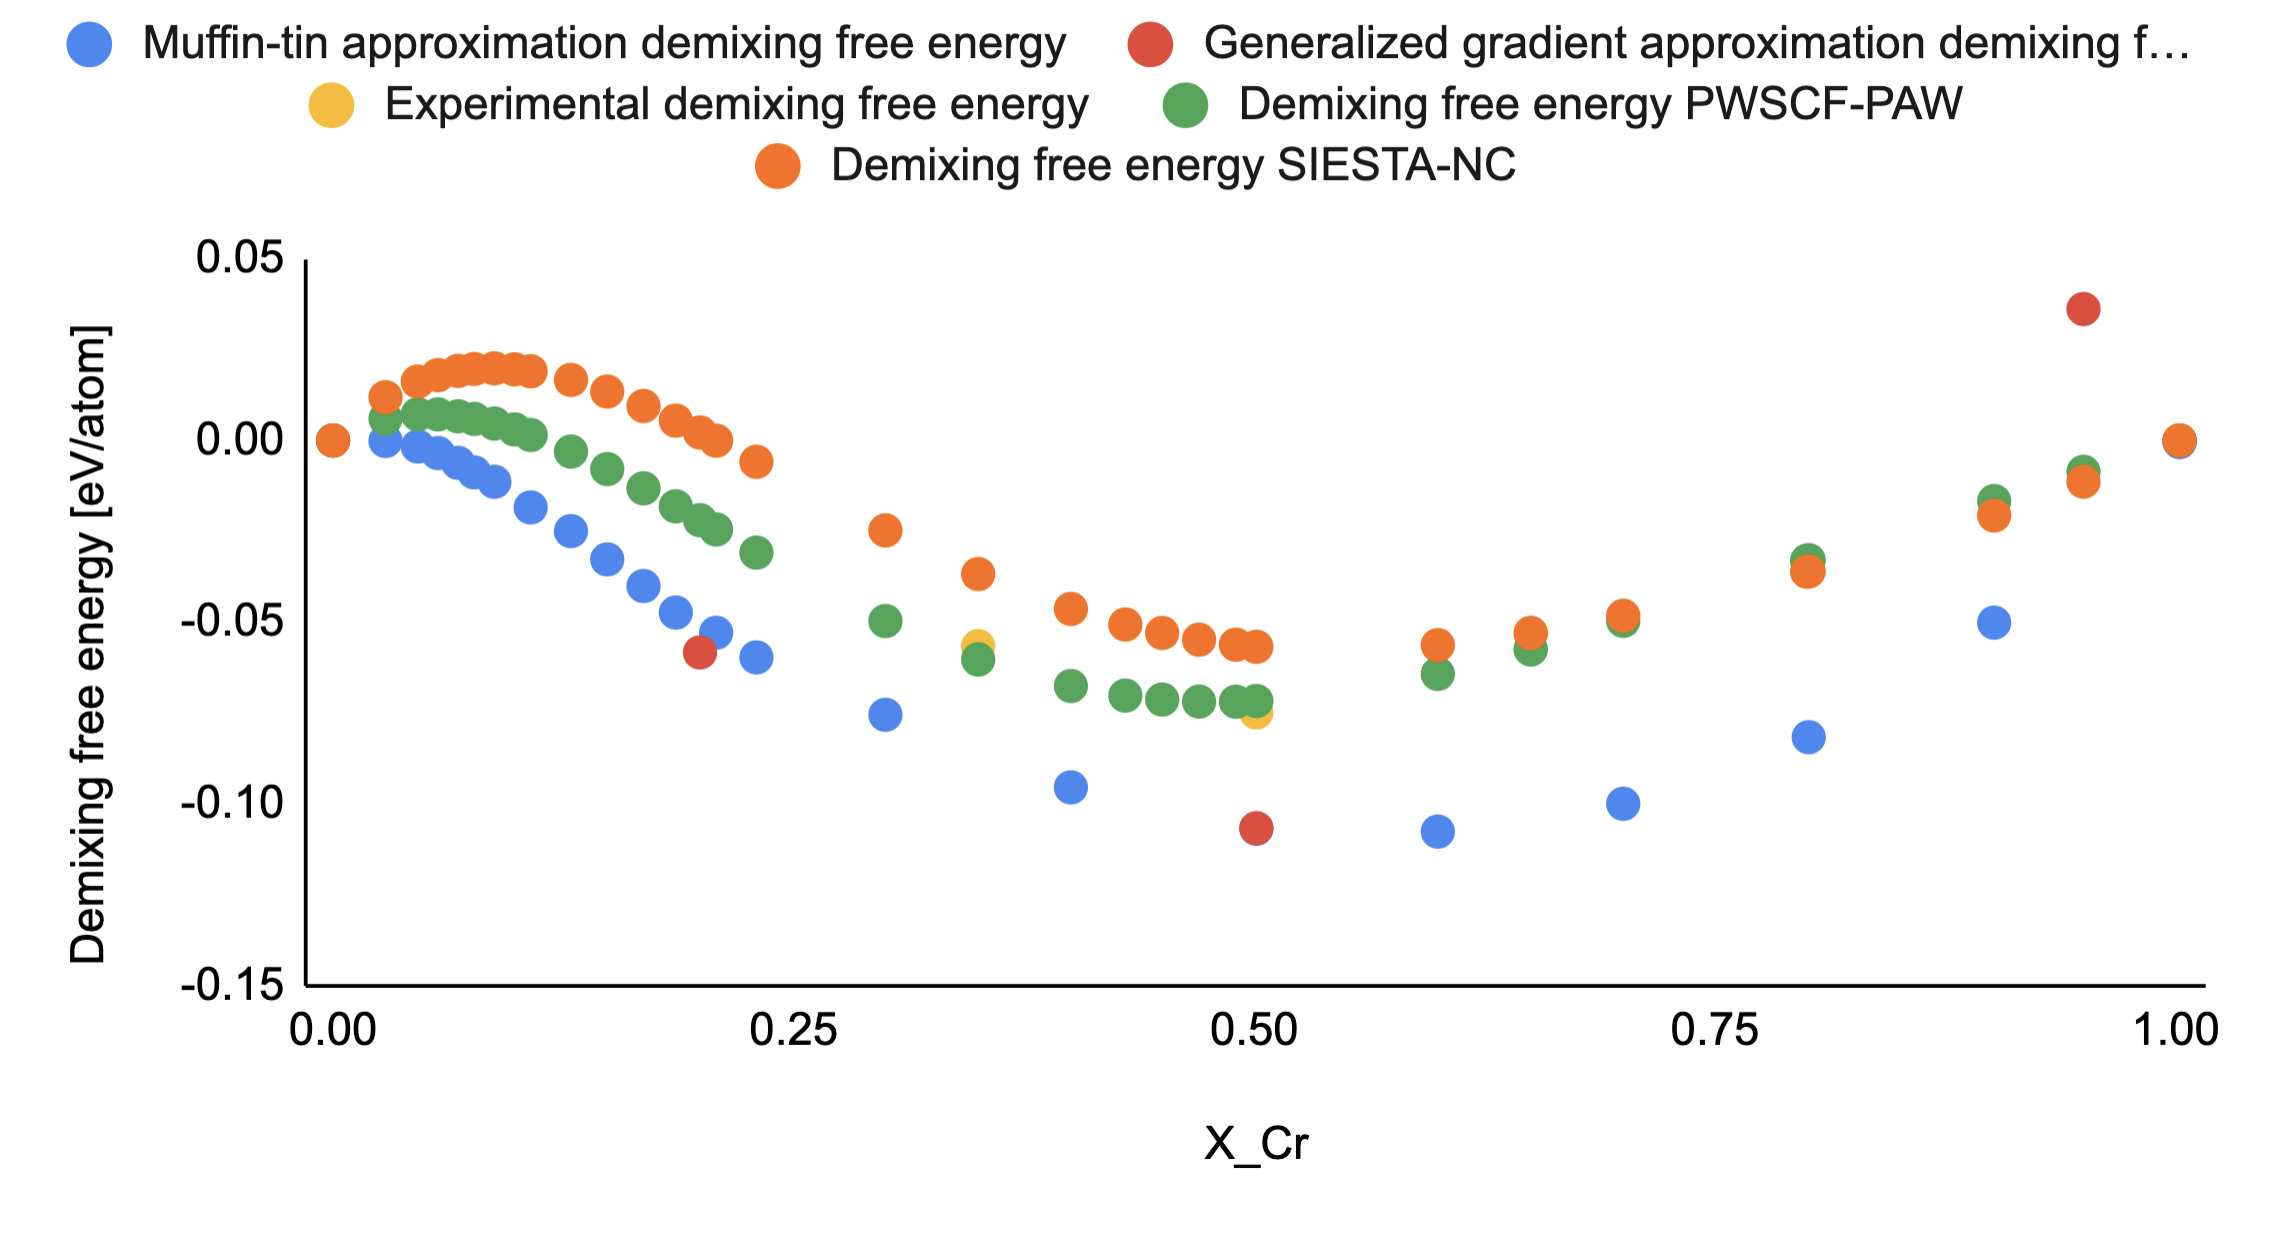
\includegraphics[width=\linewidth]{figures/dG_fig0a.png}
%DIFDELCMD < \end{subfigure}\hfill
%DIFDELCMD < \begin{subfigure}{0.48\linewidth}
%DIFDELCMD <     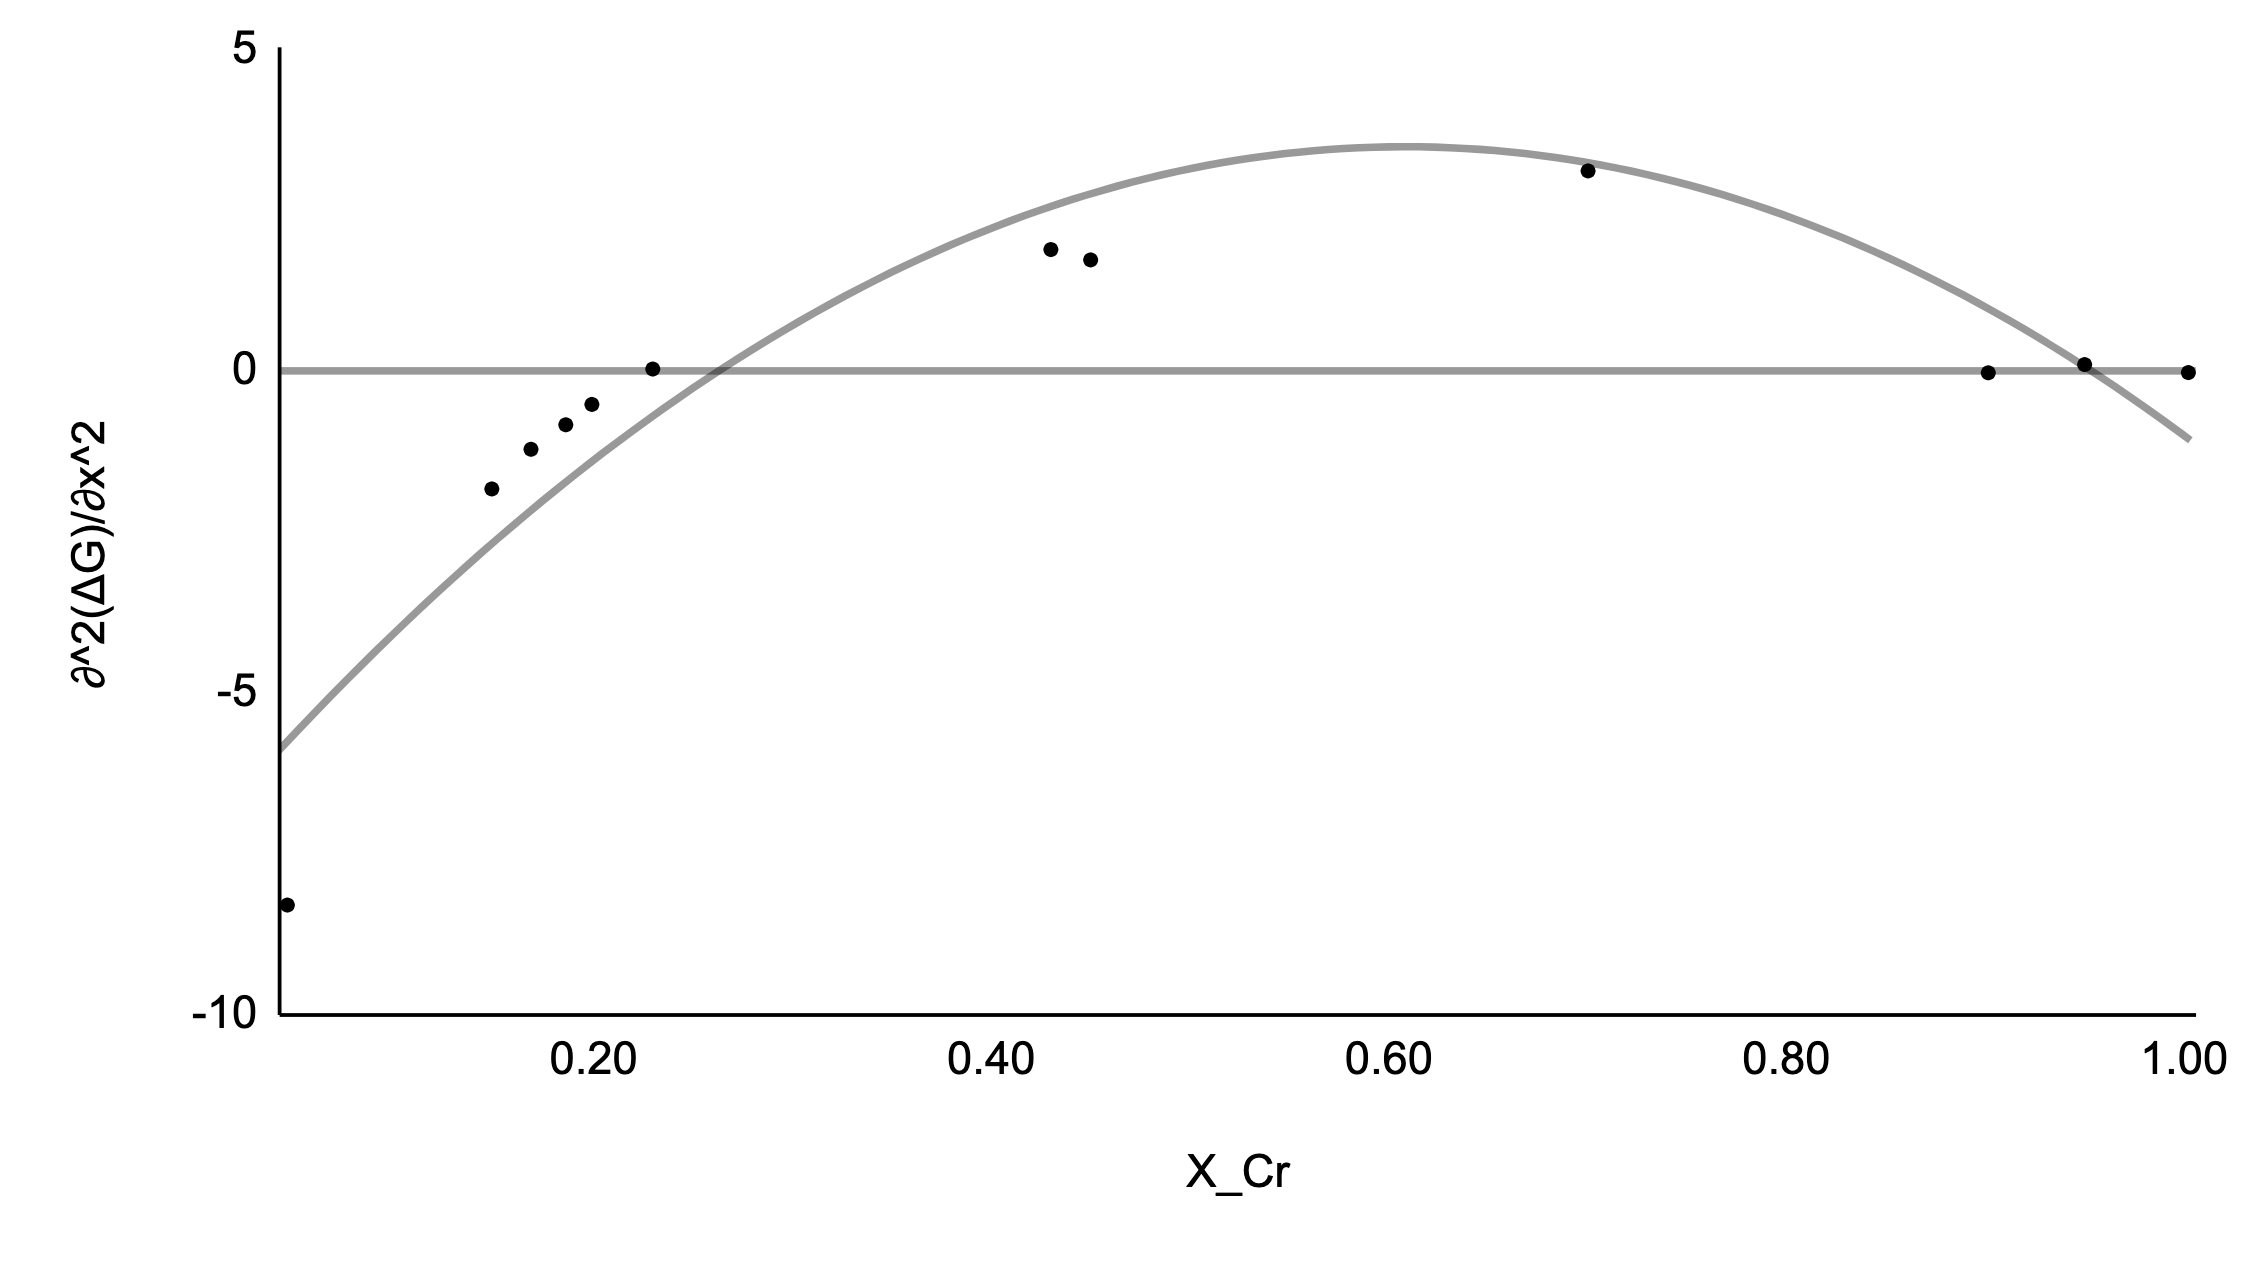
\includegraphics[width=\linewidth]{figures/ddGddx_fig0b.png}
%DIFDELCMD < \end{subfigure}
%DIFDELCMD < %%%
\DIFdelendFL \DIFaddbeginFL 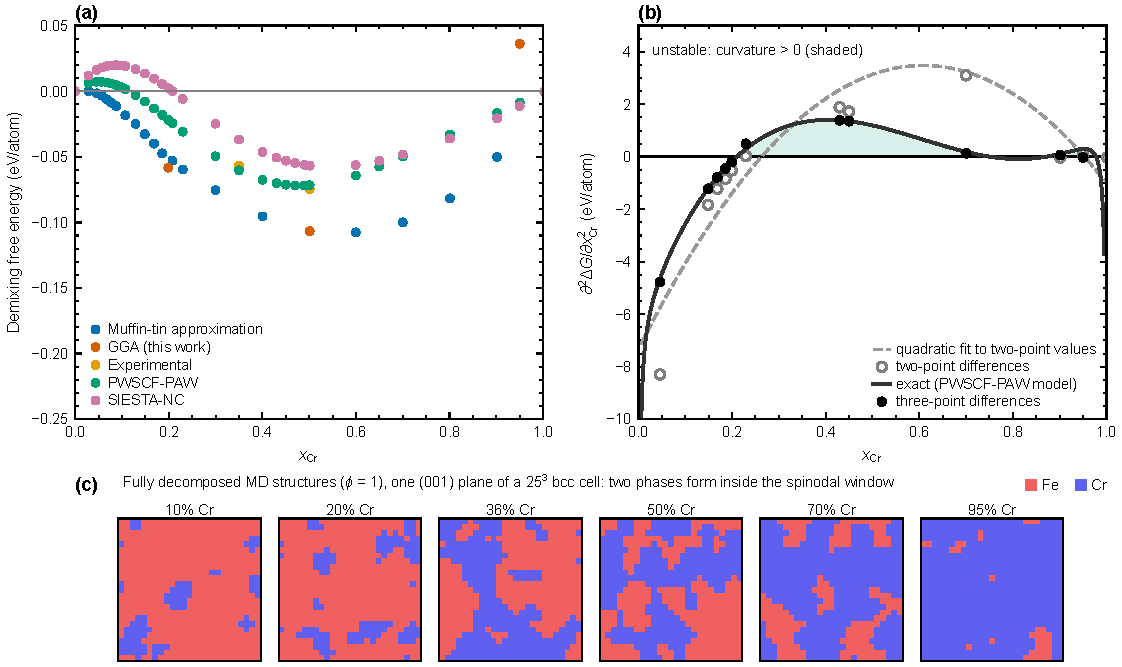
\includegraphics[width=\linewidth]{figures/kdense_scripta/with_strips/fig1_free_energy_strip.pdf}
\DIFaddendFL \caption{(a) Demixing free energy \DIFdelbeginFL \DIFdelFL{$\Delta G$ }\DIFdelendFL \DIFaddbeginFL \DIFaddFL{$\Delta G_{\mathrm{demix}} = -\Delta G_{\mathrm{mix}}$ (Eq.~\ref{eqn:demix}) }\DIFaddendFL versus chromium composition $x_{\mathrm{Cr}}$\DIFaddbeginFL \DIFaddFL{: muffin-tin approximation, GGA (present VASP calculations), experiment, and the PWSCF--PAW and SIESTA--NC interaction models of Levesque }\textit{\DIFaddFL{et al.}} \DIFaddFL{\mbox{%DIFAUXCMD
\cite{levesque2011simple} }\hskip0pt%DIFAUXCMD
at 298.15 K}\DIFaddendFL . (b) Curvature \DIFdelbeginFL \DIFdelFL{$\partial^2 \Delta G/\partial x_{\mathrm{Cr}}^2$, identifying spinodally unstable }\DIFdelendFL \DIFaddbeginFL \DIFaddFL{of the PWSCF--PAW demixing free energy. Solid line: exact analytic second derivative of the model. Filled circles: three-point second differences of its tabulated values on the non-uniform }\DIFaddendFL composition \DIFdelbeginFL \DIFdelFL{windows where }\DIFdelendFL \DIFaddbeginFL \DIFaddFL{grid. Open circles: two-point second differences of }\DIFaddendFL the \DIFaddbeginFL \DIFaddFL{same values, with a quadratic least-squares fit (dashed). Shading marks positive demixing }\DIFaddendFL curvature\DIFdelbeginFL \DIFdelFL{becomes }\DIFdelendFL \DIFaddbeginFL \DIFaddFL{, i.e., }\DIFaddendFL negative \DIFaddbeginFL \DIFaddFL{mixing curvature, which identifies spinodally unstable compositions}\DIFaddendFL . \DIFaddbeginFL \DIFaddFL{(c) One (001) atomic plane of fully decomposed ($\phi=1$) MD structures ($25^3$ }\textit{\DIFaddFL{bcc}} \DIFaddFL{cells; Sec.~\ref{sec:md}) at the indicated Cr contents; red, Fe; blue, Cr. Inside the spinodal window the alloy separates into interpenetrating Fe-rich $\alpha$ and Cr-rich $\alpha'$ domains, whereas at the dilute ends the minority element forms only isolated clusters.}\DIFaddendFL }
\label{fig:free_energy}
\end{figure}

Figure~\ref{fig:free_energy}\DIFaddbegin \DIFadd{b }\DIFaddend shows that the \DIFdelbegin \DIFdel{onset of negative curvature occurs over a finite range of chromium compositions relevant to $\delta$--ferrite in stainless steels. This thermodynamic instability defines the regime in which }\DIFdelend \DIFaddbegin \DIFadd{homogeneous alloy is unstable for $0.21 \lesssim x_{\mathrm{Cr}} \lesssim 0.75$ in the PWSCF--PAW model (with a second, narrow window at $0.87$--$0.98$); the SIESTA--NC model gives $0.25 \lesssim x_{\mathrm{Cr}} \lesssim 0.99$. Both windows contain the Fe--36Cr alloy in which spinodal decomposition was recently detected through TGS stiffening \mbox{%DIFAUXCMD
\cite{rae2026tgs}}\hskip0pt%DIFAUXCMD
. Because the entropic term lowers the curvature in proportion to $T$, these windows narrow at the higher temperatures used for aging. Within them, }\DIFaddend elastic and acoustic properties cannot be interpreted assuming a homogeneous solid solution. Instead, any observable elastic response must be understood as emerging from a system that is intrinsically driven toward compositional modulation, providing the foundation for linking free-energy curvature to stiffness evolution and ultimately to ultrasonic observables.

\subsection{Elastic stiffening and elastodynamic mapping to Rayleigh SAW observables}

% --- FIGURE: elasticity + elastodynamics ---
\begin{figure}[!h]
\centering
\DIFdelbeginFL %DIFDELCMD < \begin{subfigure}{0.48\linewidth}
%DIFDELCMD <     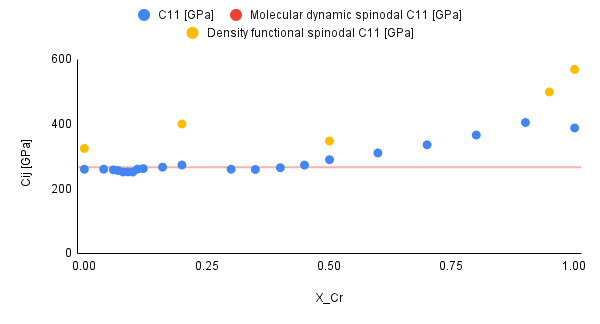
\includegraphics[width=\linewidth]{figures/Fe(1-x)Crx bcc cubic elastic tensor_fig1.png}
%DIFDELCMD < \end{subfigure}\hfill
%DIFDELCMD < \begin{subfigure}{0.48\linewidth}
%DIFDELCMD <     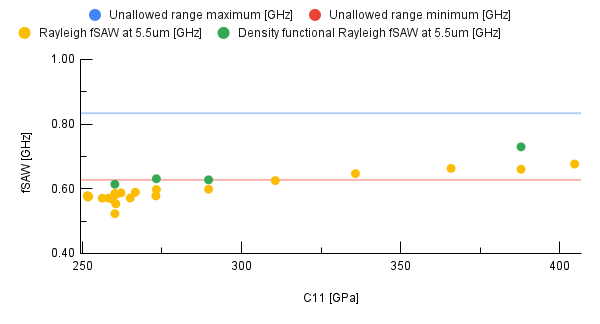
\includegraphics[width=\linewidth]{figures/Fe(1-x)Crx bcc cubic elastodynamics_fig2_ours.png}
%DIFDELCMD < \end{subfigure}
%DIFDELCMD < %%%
\DIFdelendFL \DIFaddbeginFL 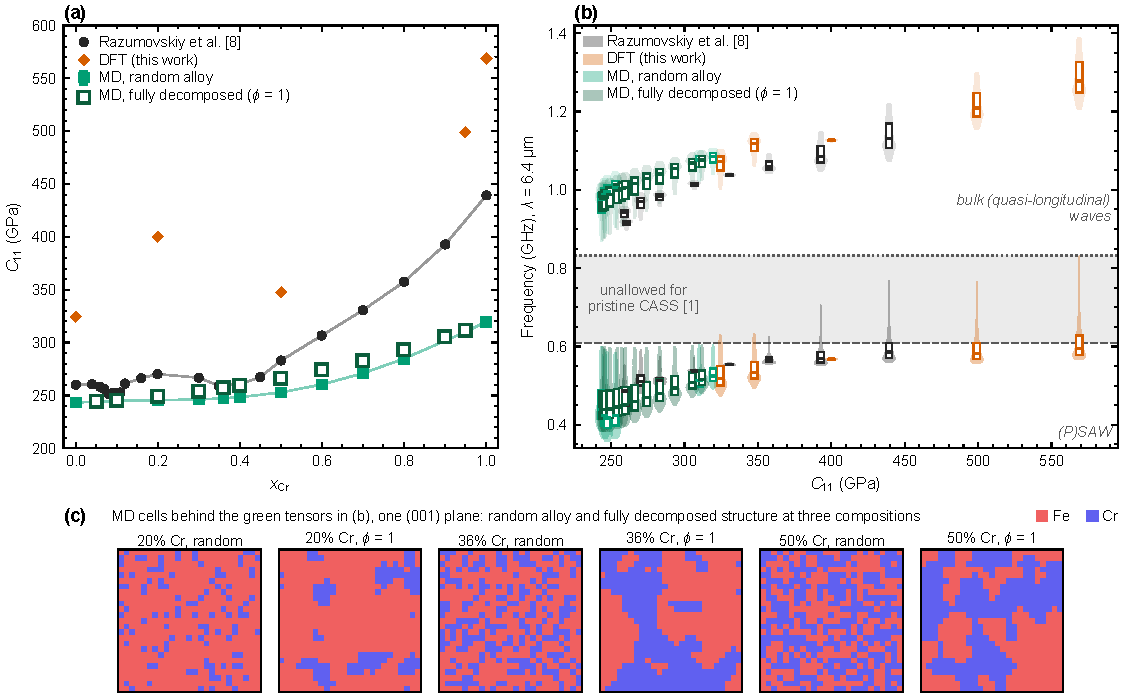
\includegraphics[width=\linewidth]{figures/kdense_scripta/with_strips/fig2_elastic_mapping_orientation_violin_bulk_mddecomp_strip.pdf}
\DIFaddendFL \caption{(a) \DIFdelbeginFL \DIFdelFL{Composition dependence }\DIFdelendFL \DIFaddbeginFL \DIFaddFL{$C_{11}$ }\DIFaddendFL of \DIFdelbeginFL \DIFdelFL{the bcc }\DIFdelendFL \DIFaddbeginFL \textit{\DIFaddFL{bcc}} \DIFaddendFL Fe$_{1-x}$Cr$_x$\DIFdelbeginFL \DIFdelFL{cubic elastic tensor}\DIFdelendFL \DIFaddbeginFL \DIFaddFL{: literature calculations of Razumovskiy }\textit{\DIFaddFL{et al.}} \DIFaddFL{\mbox{%DIFAUXCMD
\cite{razumovskiy2011first} }\hskip0pt%DIFAUXCMD
(black circles; reconstructed from digitized $C'$}\DIFaddendFL , \DIFdelbeginFL \DIFdelFL{shown for }\DIFdelendFL \DIFaddbeginFL \DIFaddFL{$C_{44}$, and $B$), present DFT calculations on 40-atom SQS (red diamonds), MD (EAM) random alloys (green squares; mean $\pm$ standard deviation of ten alloys at }\DIFaddendFL the \DIFdelbeginFL \DIFdelFL{longitudinal stiffness $C_{11}$}\DIFdelendFL \DIFaddbeginFL \DIFaddFL{DFT compositions and three elsewhere; Sec}\DIFaddendFL .\DIFaddbeginFL \DIFaddFL{~\ref{sec:md}), and fully decomposed MD structures }\DIFaddendFL (\DIFaddbeginFL \DIFaddFL{$\phi=1$, open squares; $25^3$ cells). (}\DIFaddendFL b) \DIFdelbeginFL \DIFdelFL{Elastodynamic mapping from elastic stiffness to Rayleigh surface }\DIFdelendFL \DIFaddbeginFL \DIFaddFL{Orientation-resolved }\DIFaddendFL acoustic \DIFdelbeginFL \DIFdelFL{wave frequency $f_{\mathrm{SAW}}$}\DIFdelendFL \DIFaddbeginFL \DIFaddFL{frequencies at $\lambda=6.4\,\mu$m}\DIFaddendFL , \DIFdelbeginFL \DIFdelFL{indicating elastodynamically allowed }\DIFdelendFL \DIFaddbeginFL \DIFaddFL{plotted at the $C_{11}$ of each tensor in (a). For each tensor, 10}{\DIFaddFL{,}}\DIFaddFL{000 random grain orientations were computed with the surface Green's-function method of Du }\DIFaddendFL and \DIFaddbeginFL \DIFaddFL{Zhao \mbox{%DIFAUXCMD
\cite{du2017facile}}\hskip0pt%DIFAUXCMD
, as in Ref.~\mbox{%DIFAUXCMD
\cite{al2023detecting}}\hskip0pt%DIFAUXCMD
. Lower violins: (pseudo-)SAW frequencies (pseudo-SAW retained when its intensity is at least $2\times10^{-3}$ of the SAW). Upper violins: quasi-longitudinal bulk waves along the same propagation directions. Boxes mark the interquartile range and median. The shaded band is the elastodynamically }\DIFaddendFL unallowed \DIFaddbeginFL \DIFaddFL{range of pristine 304-type CASS \mbox{%DIFAUXCMD
\cite{al2023detecting}}\hskip0pt%DIFAUXCMD
, from its maximum (pseudo-)SAW }\DIFaddendFL frequency \DIFdelbeginFL \DIFdelFL{ranges for a homogeneous solid solution}\DIFdelendFL \DIFaddbeginFL \DIFaddFL{(0.609 GHz, dashed) to its bulk-wave frequency (0.833 GHz, dotted)}\DIFaddendFL . \DIFaddbeginFL \DIFaddFL{(c) One (001) atomic plane of the MD cells behind the green tensors: random alloy and fully decomposed structure at $x_{\mathrm{Cr}}=0.20$, 0.36, and 0.50 (red, Fe; blue, Cr).}\DIFaddendFL }
\label{fig:elastic_elastodynamics}
\end{figure}

To connect thermodynamic instability to experimentally measurable quantities, we compute the cubic elastic tensor across $x_{\mathrm{Cr}}$ and propagate these elastic inputs through \DIFdelbegin \DIFdel{elastodynamic constraints relevant to surface acoustic waves.In the present geometry, }\DIFdelend \DIFaddbegin \DIFadd{the surface boundary-value problem of Sec.~2.1. Although $f_{\mathrm{SAW}}$ depends on the full tensor through $B$ and $G$, we use }\DIFaddend the longitudinal stiffness \DIFdelbegin \DIFdel{component }\DIFdelend $C_{11}$ \DIFdelbegin \DIFdel{plays a dominant role in controlling the Rayleigh SAW frequency through the dispersion relation, making it a sensitive indicator }\DIFdelend \DIFaddbegin \DIFadd{as a compact index }\DIFaddend of composition-dependent stiffening \DIFdelbegin \DIFdel{. Small overpredictions in absolute frequency are attributed to finite-size SQS representations and the absence of magnetic and chemical short-range order beyond the supercell length scale. Importantly, relative stiffening trends and peak splitting remain robust, demonstrating that first-principles elasticity captures the essential physics governing SAW observables. }\DIFdelend \DIFaddbegin \DIFadd{(Fig.~\ref{fig:elastic_elastodynamics}a). The black circles are literature calculations by Razumovskiy }\textit{\DIFadd{et al.}} \DIFadd{\mbox{%DIFAUXCMD
\cite{razumovskiy2011first}}\hskip0pt%DIFAUXCMD
, the red diamonds are ours, and the green squares are MD (EAM) random alloys computed here with the procedure of our earlier study \mbox{%DIFAUXCMD
\cite{al2023detecting}}\hskip0pt%DIFAUXCMD
; the open squares are the corresponding fully decomposed structures, which are stiffer than the random alloy at every composition, most strongly at intermediate compositions (e.g., 257.4 versus 247.3 GPa at $x_{\mathrm{Cr}}=0.36$). The present DFT tensors are systematically stiffer than the reference data (e.g., $C_{11}=324$ versus 260 GPa for }\textit{\DIFadd{bcc}} \DIFadd{Fe) and correspondingly predict higher frequencies. Possible contributors include the $\Gamma$-point-only $k$-point sampling, the finite SQS size, and the magnetic configuration. We therefore interpret relative trends rather than absolute frequencies.
}\DIFaddend 

As shown in Fig.~\ref{fig:elastic_elastodynamics}, $C_{11}$ \DIFdelbegin \DIFdel{exhibits a systematic dependence }\DIFdelend \DIFaddbegin \DIFadd{depends systematically }\DIFaddend on chromium concentration \DIFaddbegin \DIFadd{(non-monotonically in the literature and DFT data)}\DIFaddend , producing corresponding shifts in the \DIFdelbegin \DIFdel{elastodynamically allowed }\DIFdelend Rayleigh SAW frequency\DIFdelbegin \DIFdel{range. Importantly, this mapping provides a quantitative bridge between first-principles elasticity and experimentally observed SAW peak positions. }\DIFdelend \DIFaddbegin \DIFadd{. For a homogeneous solid solution, each composition corresponds to a single tensor, and hence to a single isotropic $f_{\mathrm{SAW}}$ but a distribution of (P)SAW frequencies over grain orientations. In our earlier study, elastodynamic calculations for pristine CASS over randomly sampled grain orientations defined an ``unallowed'' frequency range, above the highest (pseudo-)SAW frequency and below the bulk-wave frequency, in which no surface mode of the pristine material exists; (P)SAW peaks observed there after aging were attributed to stiffened $\delta$-ferrite \mbox{%DIFAUXCMD
\cite{al2023detecting}}\hskip0pt%DIFAUXCMD
. Figure~\ref{fig:elastic_elastodynamics}b repeats that calculation for every Fe--Cr tensor (10}{\DIFadd{,}}\DIFadd{000 grain orientations each, $\lambda=6.4\,\mu$m) \mbox{%DIFAUXCMD
\cite{du2017facile}}\hskip0pt%DIFAUXCMD
. The bulk waves of all tensors lie above the range ($\geq0.87$ GHz). In the (P)SAW branch, no literature tensor up to $x_{\mathrm{Cr}}=0.7$ and none of the MD tensors reaches it. Full decomposition raises the highest MD (P)SAW frequency, most at intermediate compositions (from 585 to 596 MHz at $x_{\mathrm{Cr}}=0.36$), but not into the range. Only the stiffest tensors enter it: Cr-rich literature alloys (9\% and 29\% of grains above 0.609 GHz at $x_{\mathrm{Cr}}=0.9$ and 1.0) and the present DFT tensors (30\% and 46\% at $x_{\mathrm{Cr}}=0.95$ and 1.0; their systematic overstiffening also places 6--8\% of grains of Fe and Fe$_{50}$Cr$_{50}$ in the range). Frequencies in this range therefore indicate stiffness beyond that of a homogeneous solid solution of $\delta$-ferrite or Fe--36Cr composition, consistent with the stiffer Cr-rich $\alpha'$ regions formed by spinodal decomposition (Fig.~\ref{fig:fsaw_combined}a). }\DIFaddend Within the spinodally unstable composition window, elastic stiffening therefore translates \DIFdelbegin \DIFdel{directly }\DIFdelend into measurable acoustic signatures, enabling stiffness changes to be inferred non-destructively.

\subsection{Separating composition trends from spinodal conversion trends}

While elastic constants vary with chromium concentration even in a homogeneous solid solution, spinodal decomposition introduces an additional, time-dependent microstructural evolution. To disentangle these effects, it is necessary to distinguish changes driven purely by composition from those arising from the progression of phase separation. We therefore report two complementary relationships that isolate these contributions within a unified elastodynamic framework.

% --- FIGURE: fSAW vs xCr and vs phi ---
\begin{figure}[!h]
\centering
\DIFdelbeginFL %DIFDELCMD < \begin{subfigure}{0.48\linewidth}
%DIFDELCMD <     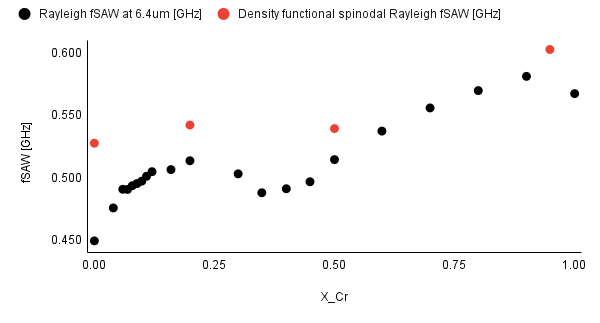
\includegraphics[width=\linewidth]{figures/Rayleigh fSAW [GHz] vs. X_Cr only_fig3.png}
%DIFDELCMD < \end{subfigure}\hfill
%DIFDELCMD < \begin{subfigure}{0.48\linewidth}
%DIFDELCMD <     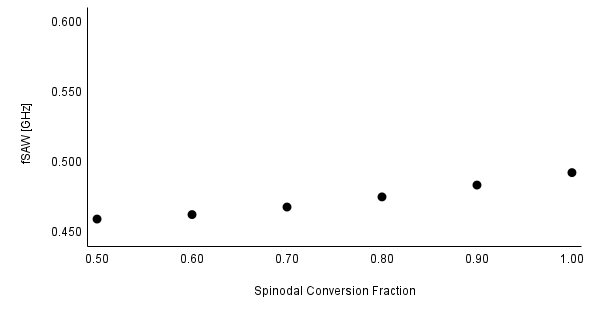
\includegraphics[width=\linewidth]{figures/Rayleigh fSAW [GHz] vs. Spinodal Conversion Fraction only_fig4.png}
%DIFDELCMD < \end{subfigure}
%DIFDELCMD < %%%
\DIFdelendFL \DIFaddbeginFL 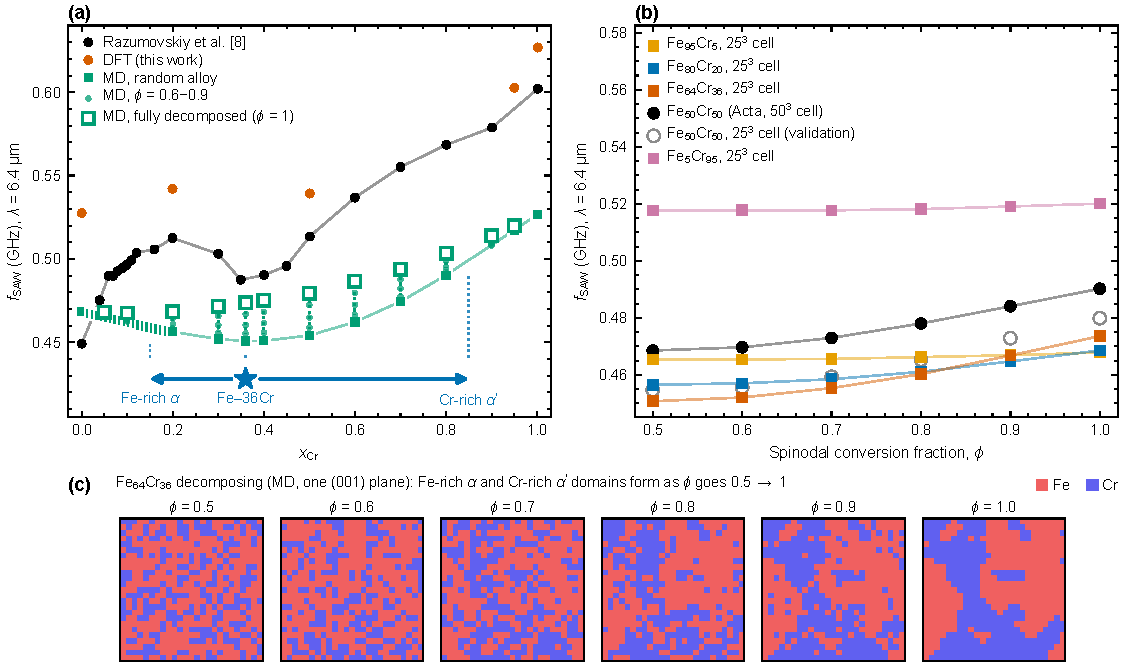
\includegraphics[width=\linewidth]{figures/kdense_scripta/with_strips/fig3_fsaw_mddecomp_6p4um_strip.pdf}
\DIFaddendFL \caption{(a) Rayleigh SAW frequency $f_{\mathrm{SAW}}$ \DIFdelbeginFL \DIFdelFL{as a function of }\DIFdelendFL \DIFaddbeginFL \DIFaddFL{versus }\DIFaddendFL chromium composition $x_{\mathrm{Cr}}$ \DIFdelbeginFL \DIFdelFL{using DFT-derived elastic constants }\DIFdelendFL (\DIFdelbeginFL \DIFdelFL{solid-solution trend}\DIFdelendFL \DIFaddbeginFL \DIFaddFL{$\lambda=6.4\,\mu$m}\DIFaddendFL ) \DIFaddbeginFL \DIFaddFL{for the literature (black), present DFT (red), and MD random-alloy (green) data of Fig}\DIFaddendFL .\DIFaddbeginFL \DIFaddFL{~\ref{fig:elastic_elastodynamics}. At each MD composition, small dots }\DIFaddendFL (\DIFdelbeginFL \DIFdelFL{b}\DIFdelendFL \DIFaddbeginFL \DIFaddFL{$\phi=0.6$--0.9}\DIFaddendFL ) \DIFdelbeginFL \DIFdelFL{Rayleigh SAW }\DIFdelendFL \DIFaddbeginFL \DIFaddFL{and an open square ($\phi=1$) show the }\DIFaddendFL frequency \DIFdelbeginFL \DIFdelFL{as a function }\DIFdelendFL of \DIFaddbeginFL \DIFaddFL{the decomposing structure, each series anchored to the random-alloy value at that composition, so the ladder height is the stiffening on decomposition (as in b). Below the data, the star marks Fe--36Cr \mbox{%DIFAUXCMD
\cite{rae2026tgs} }\hskip0pt%DIFAUXCMD
and the arrows indicate schematically the partitioning toward Fe-rich $\alpha$ and Cr-rich $\alpha'$ during }\DIFaddendFL spinodal \DIFaddbeginFL \DIFaddFL{decomposition; dotted lines rise from each composition toward the data. Arrow endpoints are illustrative, not measured phase compositions. (b) $f_{\mathrm{SAW}}$ versus spinodal }\DIFaddendFL conversion fraction $\phi$ from \DIFdelbeginFL \DIFdelFL{molecular dynamics, isolating microstructural evolution effects during }\DIFdelendFL \DIFaddbeginFL \DIFaddFL{the MD (EAM) }\DIFaddendFL decomposition \DIFaddbeginFL \DIFaddFL{simulations (Sec}\DIFaddendFL .\DIFaddbeginFL \DIFaddFL{~\ref{sec:md}): equiatomic Fe$_{50}$Cr$_{50}$ from Ref.~\mbox{%DIFAUXCMD
\cite{al2023detecting} }\hskip0pt%DIFAUXCMD
(black, $50^3$ cell, fixed density 7535 kg m$^{-3}$), and Fe$_{95}$Cr$_{5}$, Fe$_{80}$Cr$_{20}$, Fe$_{64}$Cr$_{36}$, and Fe$_{5}$Cr$_{95}$ from the present $25^3$-cell calculations (squares); open circles repeat Fe$_{50}$Cr$_{50}$ in the $25^3$ cell as a check. $\phi=0.5$ is the random alloy and $\phi=1$ the fully separated structure. (c) One (001) atomic plane of the $25^3$ MD cell of Fe$_{64}$Cr$_{36}$ from $\phi=0.5$ to 1.0 (red, Fe; blue, Cr): Fe-rich $\alpha$ and Cr-rich $\alpha'$ domains form and coarsen as $\phi$ increases; these are the structures whose frequencies are plotted in (b).}\DIFaddendFL }
\label{fig:fsaw_combined}
\end{figure}

Figure~\ref{fig:fsaw_combined}\DIFdelbegin \DIFdel{demonstrates that while }\DIFdelend \DIFaddbegin \DIFadd{a shows how chromium partitioning produces stiffening. The Fe--36Cr composition lies near a local minimum of the homogeneous }\DIFaddend $f_{\mathrm{SAW}}(x_{\mathrm{Cr}})$ \DIFaddbegin \DIFadd{curve. Spinodal decomposition moves material toward Fe-rich $\alpha$ and Cr-rich $\alpha'$ compositions (arrows); in both directions the homogeneous-alloy frequency increases. The DFT set, with only five compositions, is consistent with this non-monotonic dependence but cannot resolve the minimum. The MD random alloys, an independent classical model, also show a frequency minimum, at $x_{\mathrm{Cr}}\approx0.36$--0.40, i.e.\ at the Fe--36Cr composition, even though their $C_{11}$ increases monotonically (Fig.~\ref{fig:elastic_elastodynamics}a): the minimum comes from the shear moduli, which control the Rayleigh velocity ($C_{44}$ decreases from 116 GPa for Fe to 106 GPa at $x_{\mathrm{Cr}}=0.5$). $C_{11}$ is therefore a convenient index of stiffening, but the SAW response is governed by shear stiffness. Figure~\ref{fig:fsaw_combined}a describes the properties of the constituents; the effective response of the two-phase microstructure additionally depends on phase fractions and on the domain size relative to the SAW wavelength.
}

\DIFadd{Figure~\ref{fig:fsaw_combined}b isolates the effect of decomposition at fixed overall composition (Fe$_{50}$Cr$_{50}$). In the MD (EAM) simulations, $f_{\mathrm{SAW}}$ increases monotonically from 0.469 GHz for the random alloy ($\phi=0.5$) to 0.490 GHz for the fully separated structure ($\phi=1$), an increase of about 4.6\% under the fixed-density assumption. The empirical-potential and first-principles results therefore agree in sign. Repeating the decomposition at twelve compositions from $x_{\mathrm{Cr}}=0.05$ to 0.95 (Sec.~\ref{sec:md}) gives frequency increases between the random and fully separated states that are nearly symmetric about the equiatomic composition: 0.5\%, 1.1\%, 2.6\%, 4.4\%, 5.1\%, 5.4\%, and 5.5\% for $x_{\mathrm{Cr}}=0.05$, 0.10, 0.20, 0.30, 0.36, 0.40, and 0.50, and 5.3\%, 4.1\%, 2.7\%, 1.1\%, and 0.5\% for $x_{\mathrm{Cr}}=0.60$, 0.70, 0.80, 0.90, and 0.95. Stiffening on decomposition is therefore largest within the spinodally unstable window of Fig.~\ref{fig:free_energy}b, including the Fe--36Cr composition, and nearly vanishes for the dilute alloys at either end. The fully separated state is an idealized limit, so these values bound the stiffening from above. At 50/50, the small-cell series lies about 2\% below the original series in absolute frequency because the original moduli used a different isotropic average; the relative changes agree to within one percentage point. Together, $f_{\mathrm{SAW}}(x_{\mathrm{Cr}})$ }\DIFaddend captures the baseline elastic response of a homogeneous alloy, \DIFdelbegin \DIFdel{the evolution of }\DIFdelend \DIFaddbegin \DIFadd{and }\DIFaddend $f_{\mathrm{SAW}}(\phi)$ reflects \DIFaddbegin \DIFadd{the }\DIFaddend additional stiffening associated with progressive spinodal conversion. This separation enables experimental SAW measurements to be interpreted in terms of both composition and decomposition state, providing a pathway to distinguish early-stage spinodal evolution from equilibrium compositional effects.


\section{Discussion}

Taken together, the results establish a closed thermodynamics-to-observable pathway for interpreting picosecond ultrasonic measurements in $\delta$--ferrite–containing stainless steels. The free-energy curvature criterion identifies the composition window in which the homogeneous solid solution is intrinsically unstable, defining the regime where elastic and acoustic properties must reflect ongoing or incipient spinodal decomposition rather than equilibrium alloy behavior.

Within this thermodynamically unstable regime, first-principles elasticity reveals systematic stiffening trends that are propagated through elastodynamic constraints into Rayleigh SAW frequency shifts. The direct mapping between elastic constants and SAW observables provides a quantitative basis for interpreting peak shifts and splitting as signatures of stiffness evolution, rather than purely phenomenological indicators.

Crucially, separating the solid-solution trend $f_{\mathrm{SAW}}(x_{\mathrm{Cr}})$ from the spinodal conversion trend $f_{\mathrm{SAW}}(\phi)$ resolves a key ambiguity in experimental interpretation. While composition alone can shift SAW frequencies, progressive spinodal decomposition introduces additional stiffening that cannot be captured by composition-dependent elasticity alone. The combined framework therefore enables SAW peak splitting to be interpreted as a mechanistically grounded indicator of microstructural evolution toward embrittlement, rather than as a purely compositional effect.

This separation clarifies why SAW peak splitting emerges as a robust, non-destructive diagnostic of spinodal decomposition in CASS and related alloys, and suggests a general strategy for extending ultrasonic embrittlement detection to other phase-separating structural materials.


\section{Conclusions}
We presented a compact thermodynamics-to-elastodynamics workflow for bcc Fe--Cr $\delta$--ferrite that links demixing free-energy curvature, first-principles elastic constants, and Rayleigh SAW observables. Free-energy curvature provides a direct stability criterion that identifies spinodally unstable composition windows. DFT-derived cubic elasticity quantifies composition-dependent stiffening trends and supplies inputs for elastodynamic prediction. Combining these elements yields experimentally actionable relationships for interpreting picosecond ultrasonics across both composition and decomposition-state variables.

\DIFaddbegin \section*{\DIFadd{Data Availability}}
\DIFadd{The tabulated data, the atomistic and first-principles simulation inputs and outputs, and the scripts that generate all figures will be made publicly available at }\url{https://github.com/saleemaldajani/elastopya}\DIFadd{, with an archived DOI.
}


\DIFaddend \bibliographystyle{elsarticle-num}
\bibliography{references}


\newpage
\clearpage

\section*{Supplementary Material}
\DIFdelbegin \DIFdel{The following material retains the original draft figures }\DIFdelend \DIFaddbegin 

\setcounter{figure}{0}
\renewcommand{\thefigure}{S\arabic{figure}}

\subsection*{\DIFadd{S1. Thermal transport estimates}}

\DIFadd{Thermal properties in Fig.~\ref{fig5} are estimated with the Debye model, and a lower limit for the thermal conductivity is obtained at high temperature \mbox{%DIFAUXCMD
\cite{clarke2003materialsselection,clarke2003materialsdesign}}\hskip0pt%DIFAUXCMD
:
}\begin{eqnarray}
    \DIFadd{\kappa }&\DIFadd{=}& \DIFadd{\frac{1}{3} C_v v_m \Lambda }\\
    \DIFadd{\kappa_{min} \rightarrow k_B v_m \Lambda \rightarrow k_B v_m \Lambda_{min} }&\DIFadd{=}& \DIFadd{A k_B \left(\frac{N_A m}{M}\right)^{\frac{2}{3}} \rho^{\frac{1}{6}} E^{\frac{1}{2}} }\\
    \DIFadd{\Theta_D }&\DIFadd{=}& \DIFadd{\frac{2\hbar v_m}{a_0 k_B} \rightarrow B_D \frac{\hbar}{k_B} \left(\frac{N_A m}{M}\right)^{\frac{1}{3}} \frac{E^{\frac{1}{2}} }{\rho^{\frac{1}{6}}}
}\end{eqnarray}
\DIFadd{where $\kappa$ is thermal conductivity, $\Theta_D$ is the Debye temperature, $C_v$ is the heat capacity at constant volume, $v_m$ is the average acoustic velocity, $\Lambda$ is the phonon mean free path, $m$ is the number of atoms, $M$ is the mass, $\rho$ is the density, and $E$ is Young's modulus. The constants $A$ and $B_D$ arise from approximating $v_m$ as proportional to $\sqrt{E/\rho}$; we use $A=0.87$ following Clarke \mbox{%DIFAUXCMD
\cite{clarke2003materialsselection}}\hskip0pt%DIFAUXCMD
. A temperature-dependent alternative is the Cahill--Watson--Pohl model, $\kappa_{min} (T) = (\frac{\pi}{6})^{\frac{1}{3}} k_B n^{\frac{2}{3}} \sum_{i} v_i (\frac{T}{\Theta_i})^2 \int_{0}^{\Theta_i/T} \frac{x^3 e^x}{(e^x -1)^2}\,dx$ with $\Theta_i = v_i (\hbar/k_B) (6\pi^2n)^{\frac{1}{3}}$ \mbox{%DIFAUXCMD
\cite{cahill1992lower}}\hskip0pt%DIFAUXCMD
.
}

\subsection*{\DIFadd{S2. Additional figures}}
\DIFadd{The following figures are retained from the original draft }\DIFaddend for completeness and traceability.
\DIFdelbegin \DIFdel{All figure numbering in this supplementary section is independent of the main manuscript.
}\DIFdelend 



\DIFdelbegin %DIFDELCMD < \setcounter{figure}{0}
%DIFDELCMD < \renewcommand{\thefigure}{S\arabic{figure}}
%DIFDELCMD < 

%DIFDELCMD < %%%
\DIFdelend \begin{figure}[!ht]
\centering
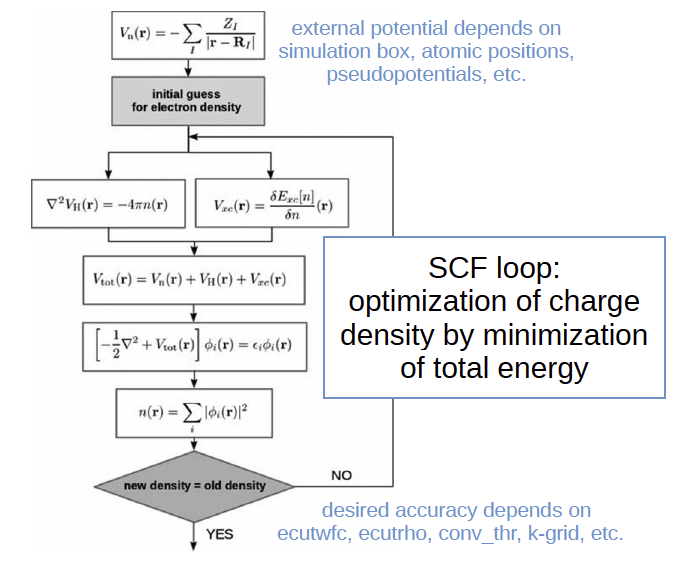
\includegraphics[width=0.85\textwidth]{figures/SCF.png}
\caption{\DIFaddbeginFL \DIFaddFL{Self-consistent field (}\DIFaddendFL SCF\DIFaddbeginFL \DIFaddFL{) }\DIFaddendFL loop schematic illustrating self-consistent electronic-structure workflow \cite{giustino2014materials}.}
\label{fig:SCF-loop}
\end{figure}


\begin{figure}[h!]
    \centering
    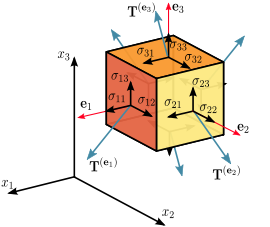
\includegraphics[width=0.6\textwidth]{Parts/Figures/Cij.png}
    \caption{Stress tensor visualization \cite{al2020non}.}
    \label{fig:seis-refl-tech}
\end{figure}

\begin{figure}[!ht]
	\centering
	\begin{subfigure}{0.9\textwidth}
         \centering
         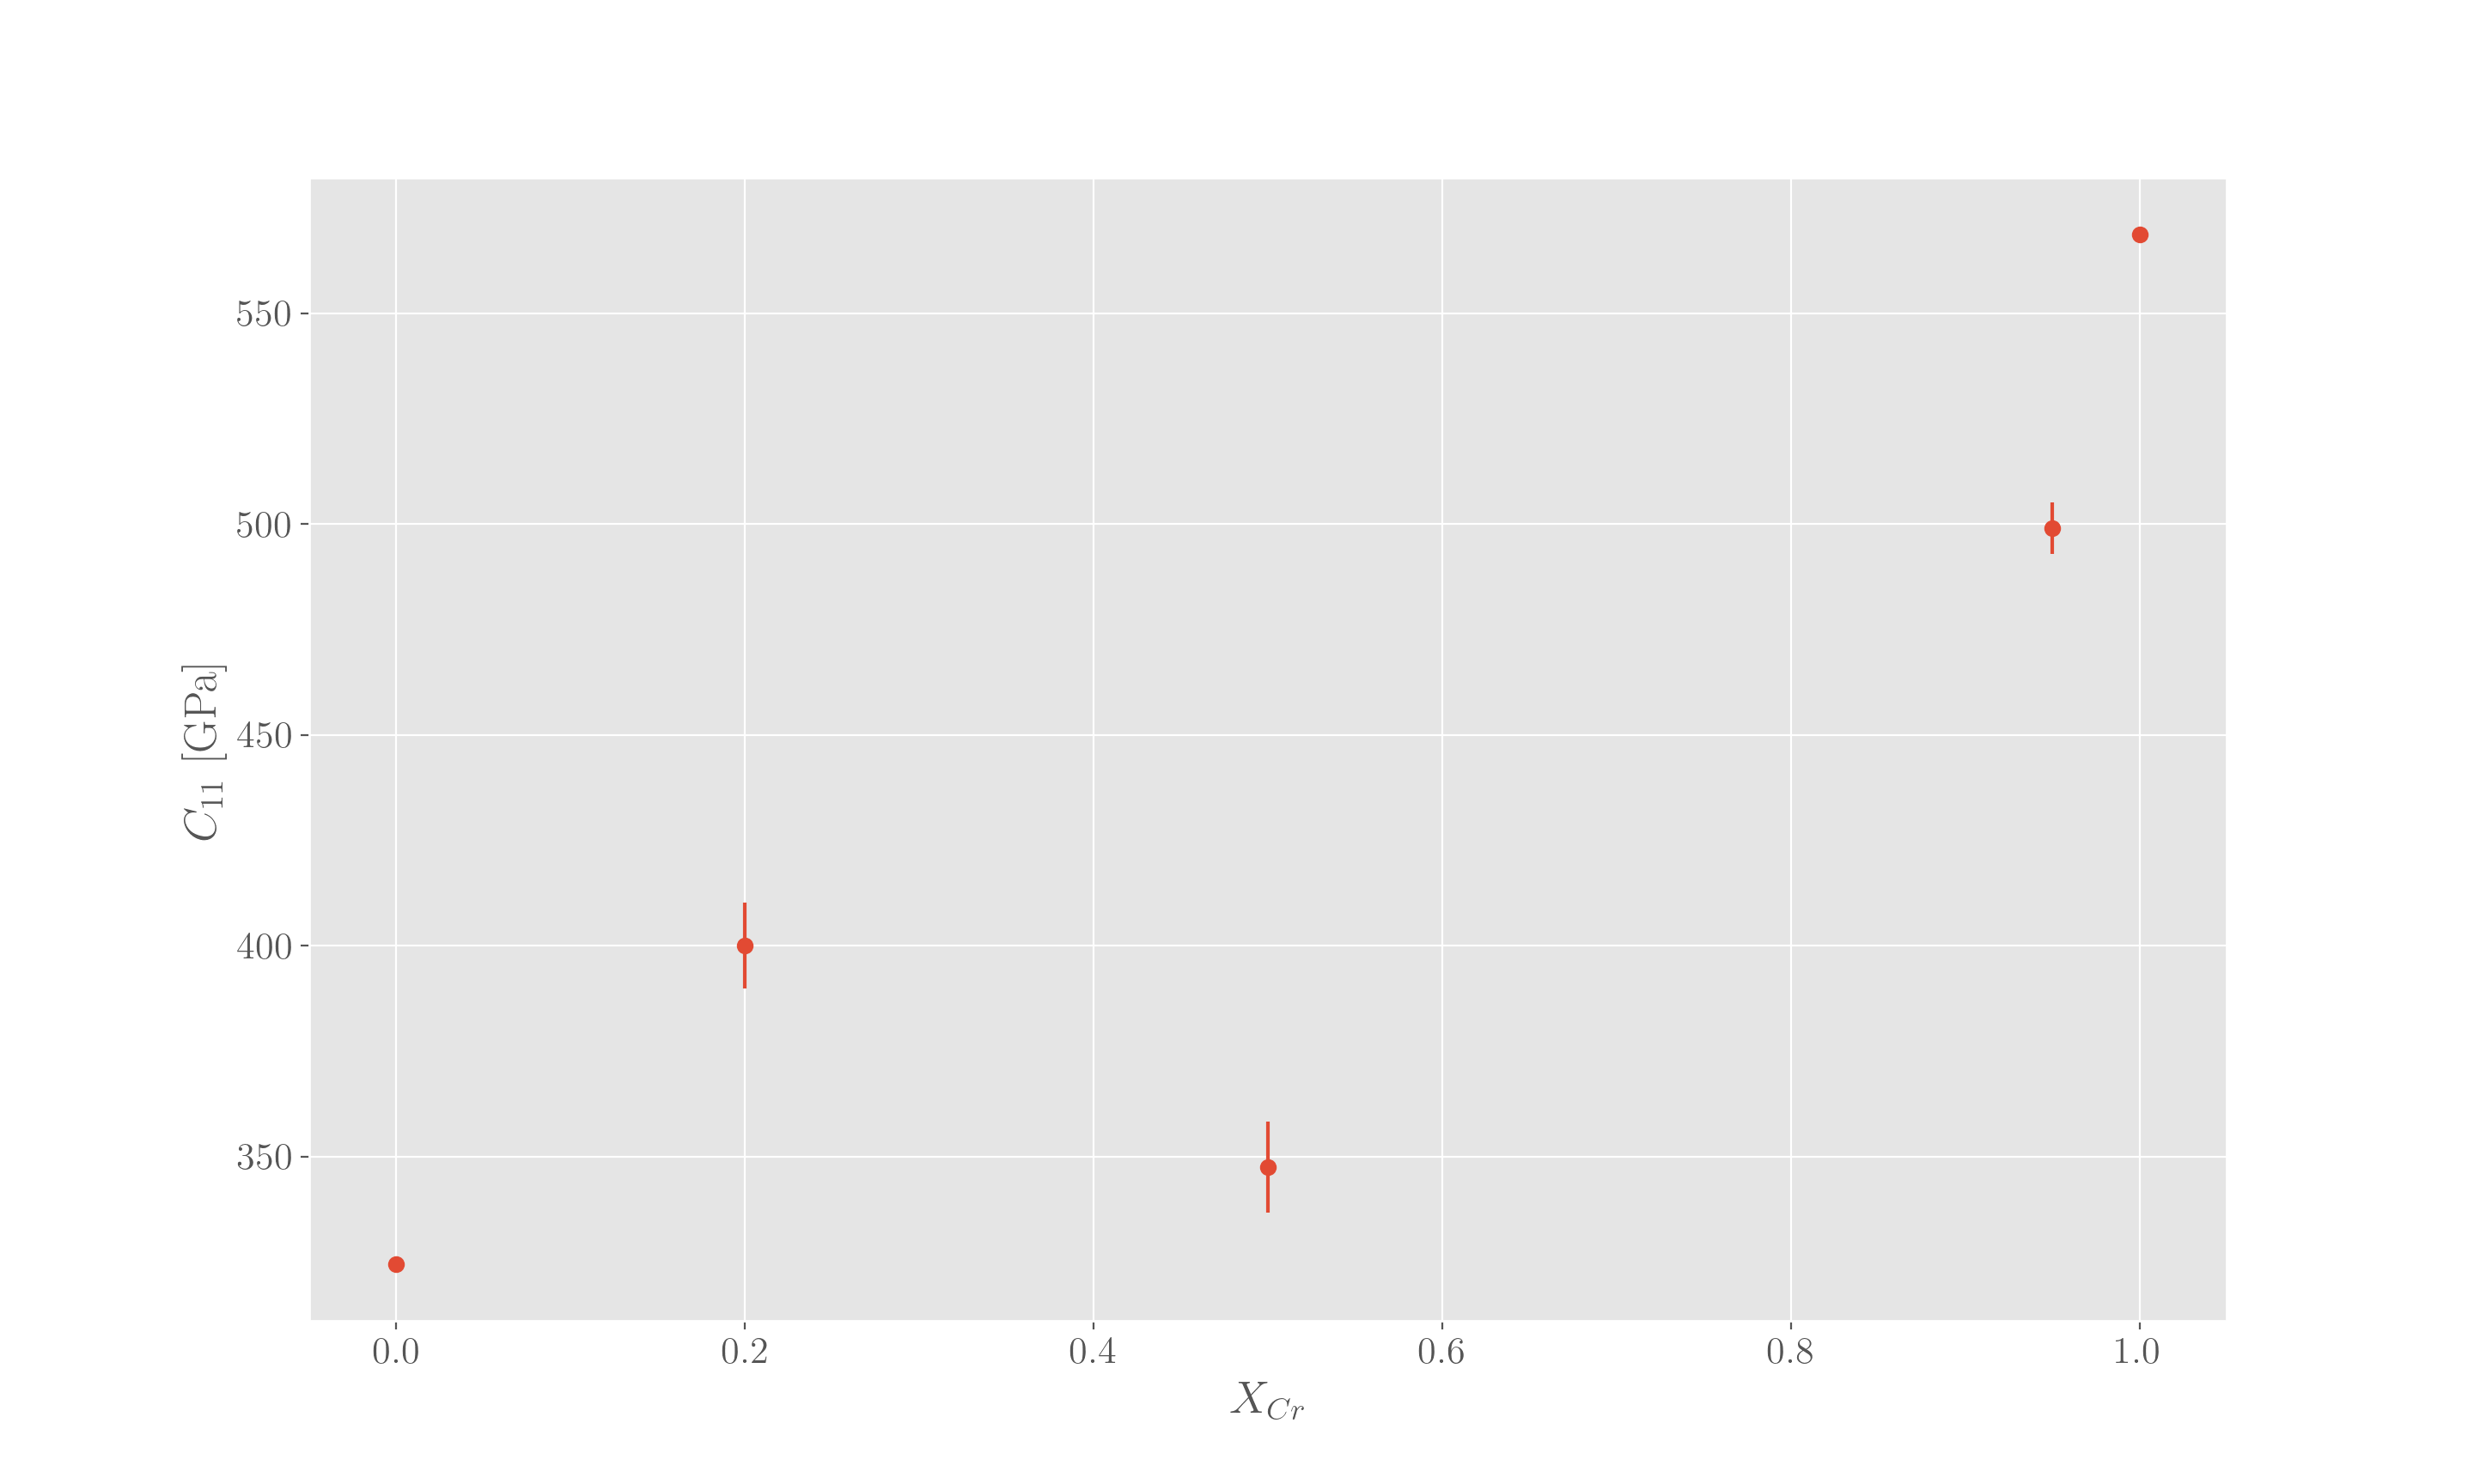
\includegraphics[width=\linewidth]{Parts/Figures/C11.png}
         \caption{Normal constant, \(C_{11}\), illustrating the longitudinal stiffness of bcc binary FeCr alloy as a function of chromium composition. This stiffness parameter is crucial for understanding the acoustic velocity and mechanical properties of the material.}
         \label{fig1a}
     \end{subfigure}
     \hfill
     \begin{subfigure}{0.45\textwidth}
         \centering
         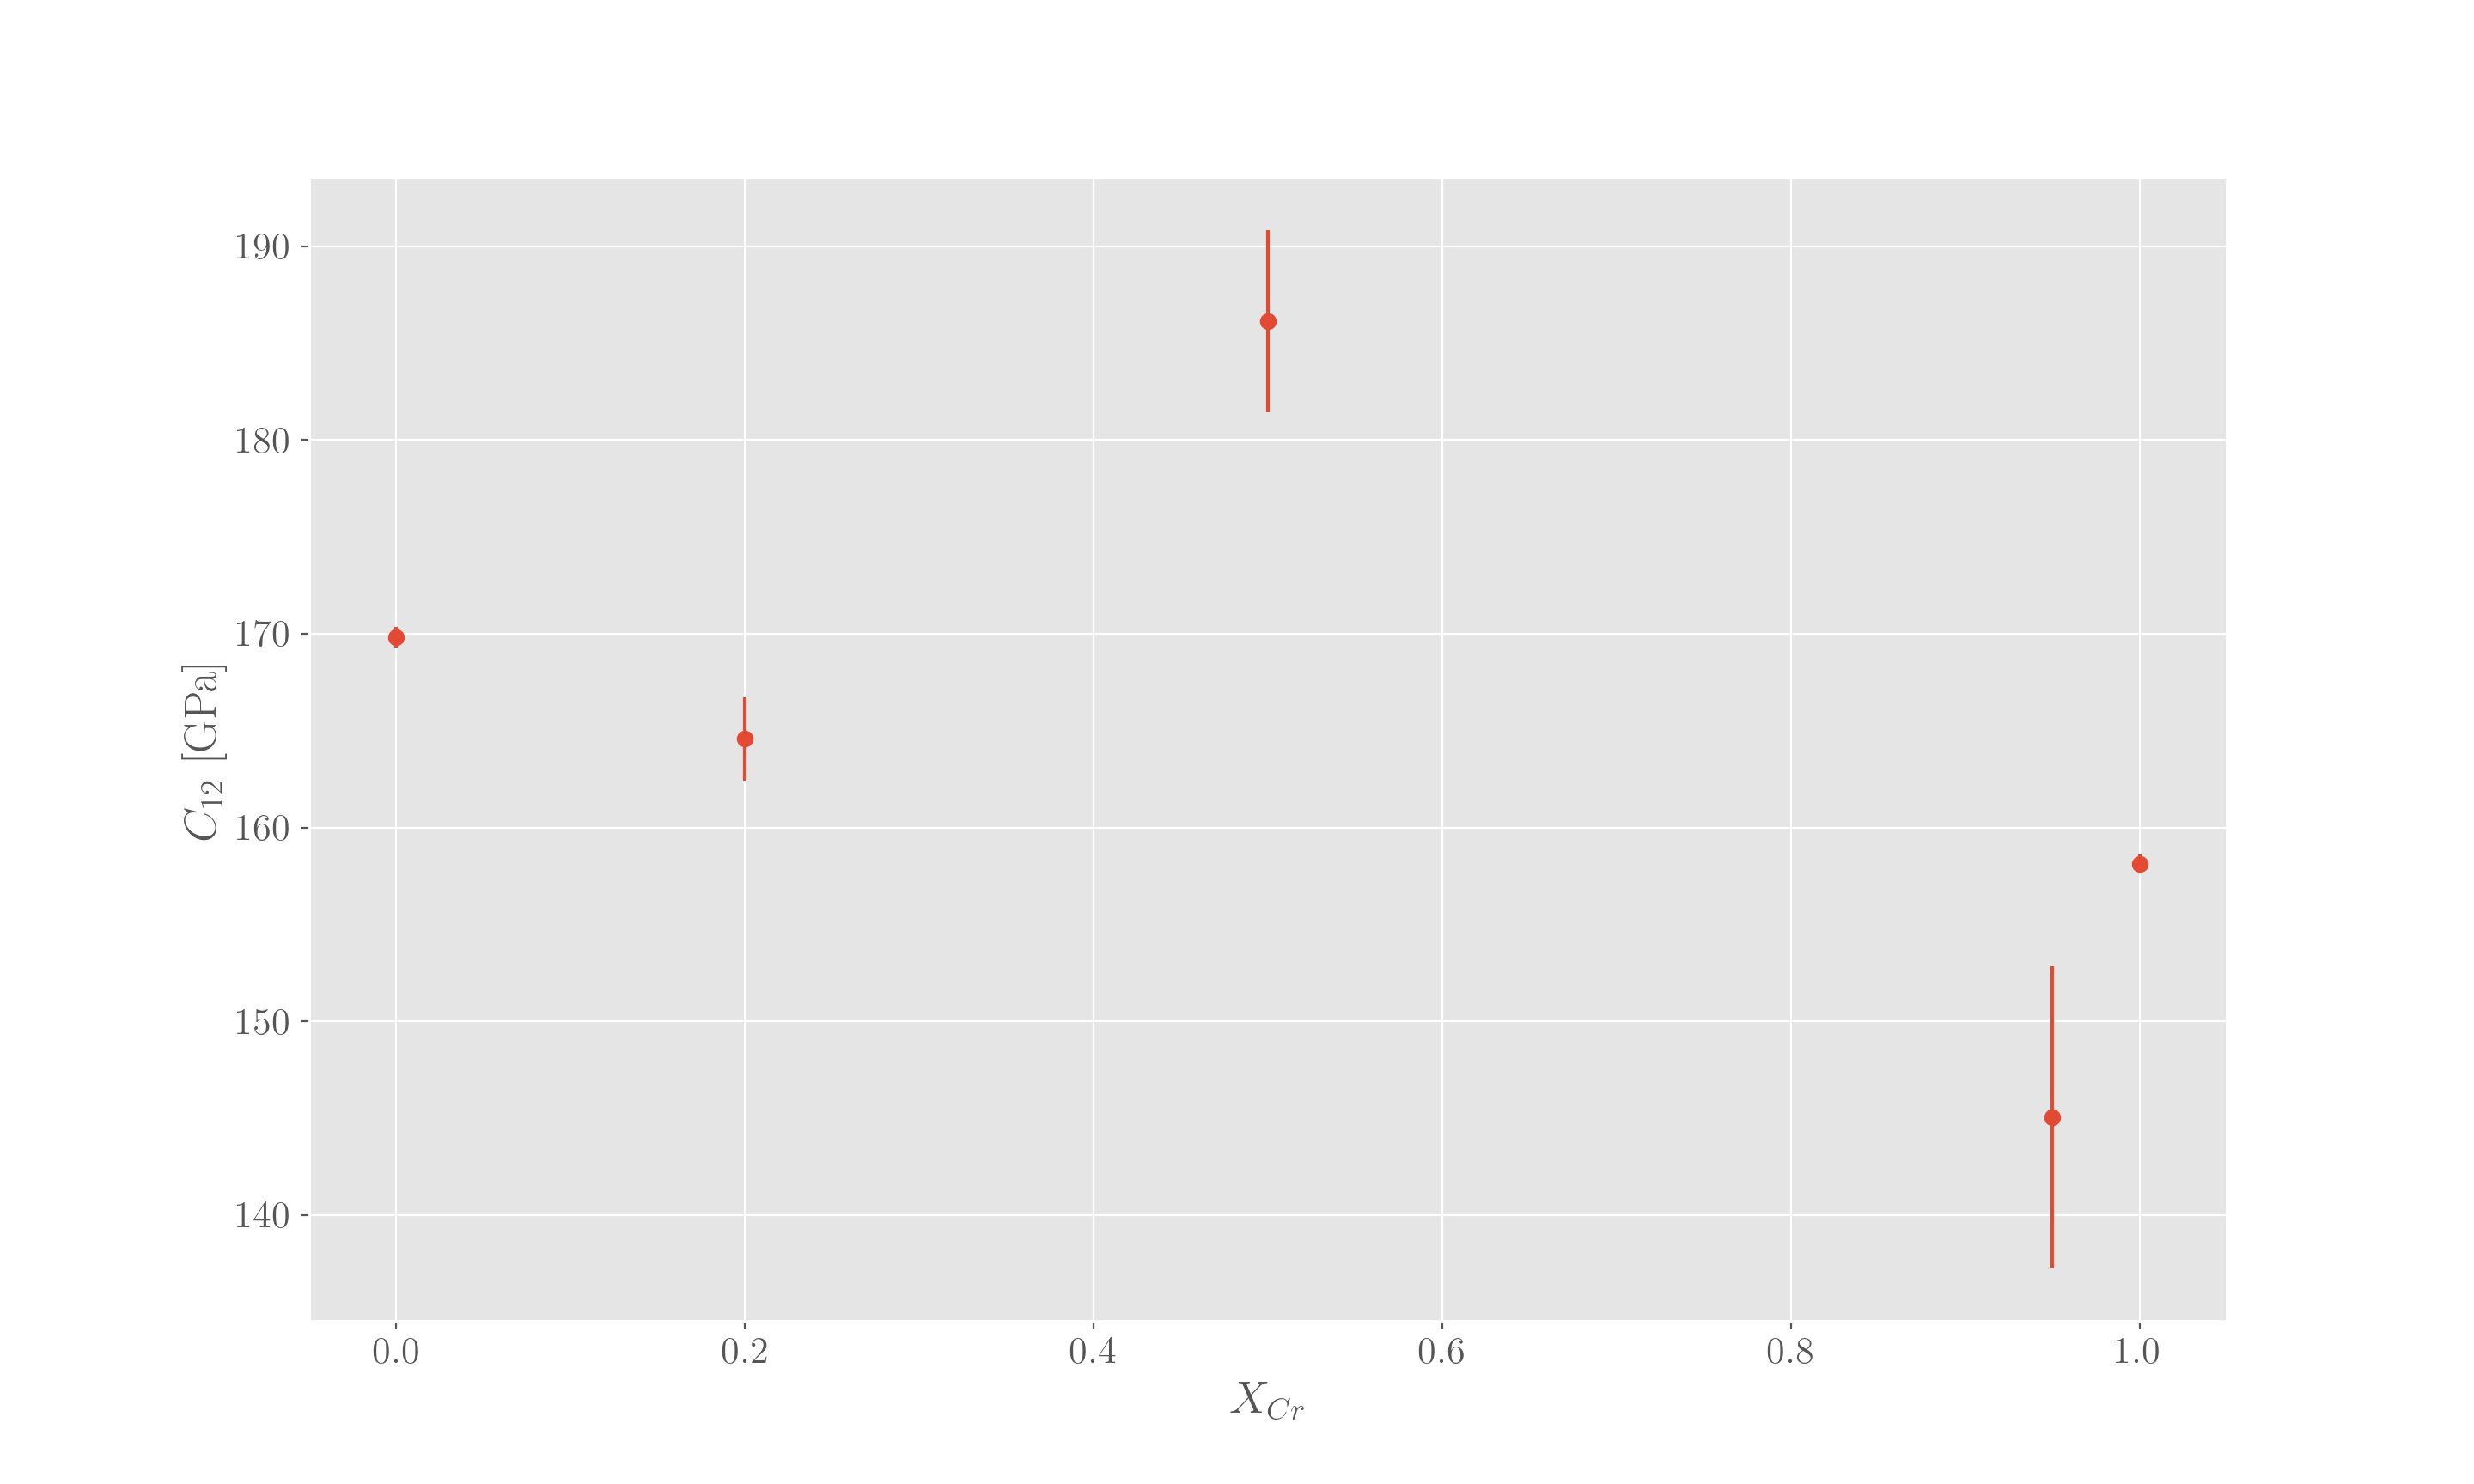
\includegraphics[width=\linewidth]{Parts/Figures/C12.png}
         \caption{The interplanar elastic constant \(C_{12}\), showing the coupling between axial and lateral strains, indicative of the alloy's resistance to shear along crystallographic planes.}
         \label{fig1b}
     \end{subfigure}
     \hfill
     \begin{subfigure}{0.45\textwidth}
         \centering
         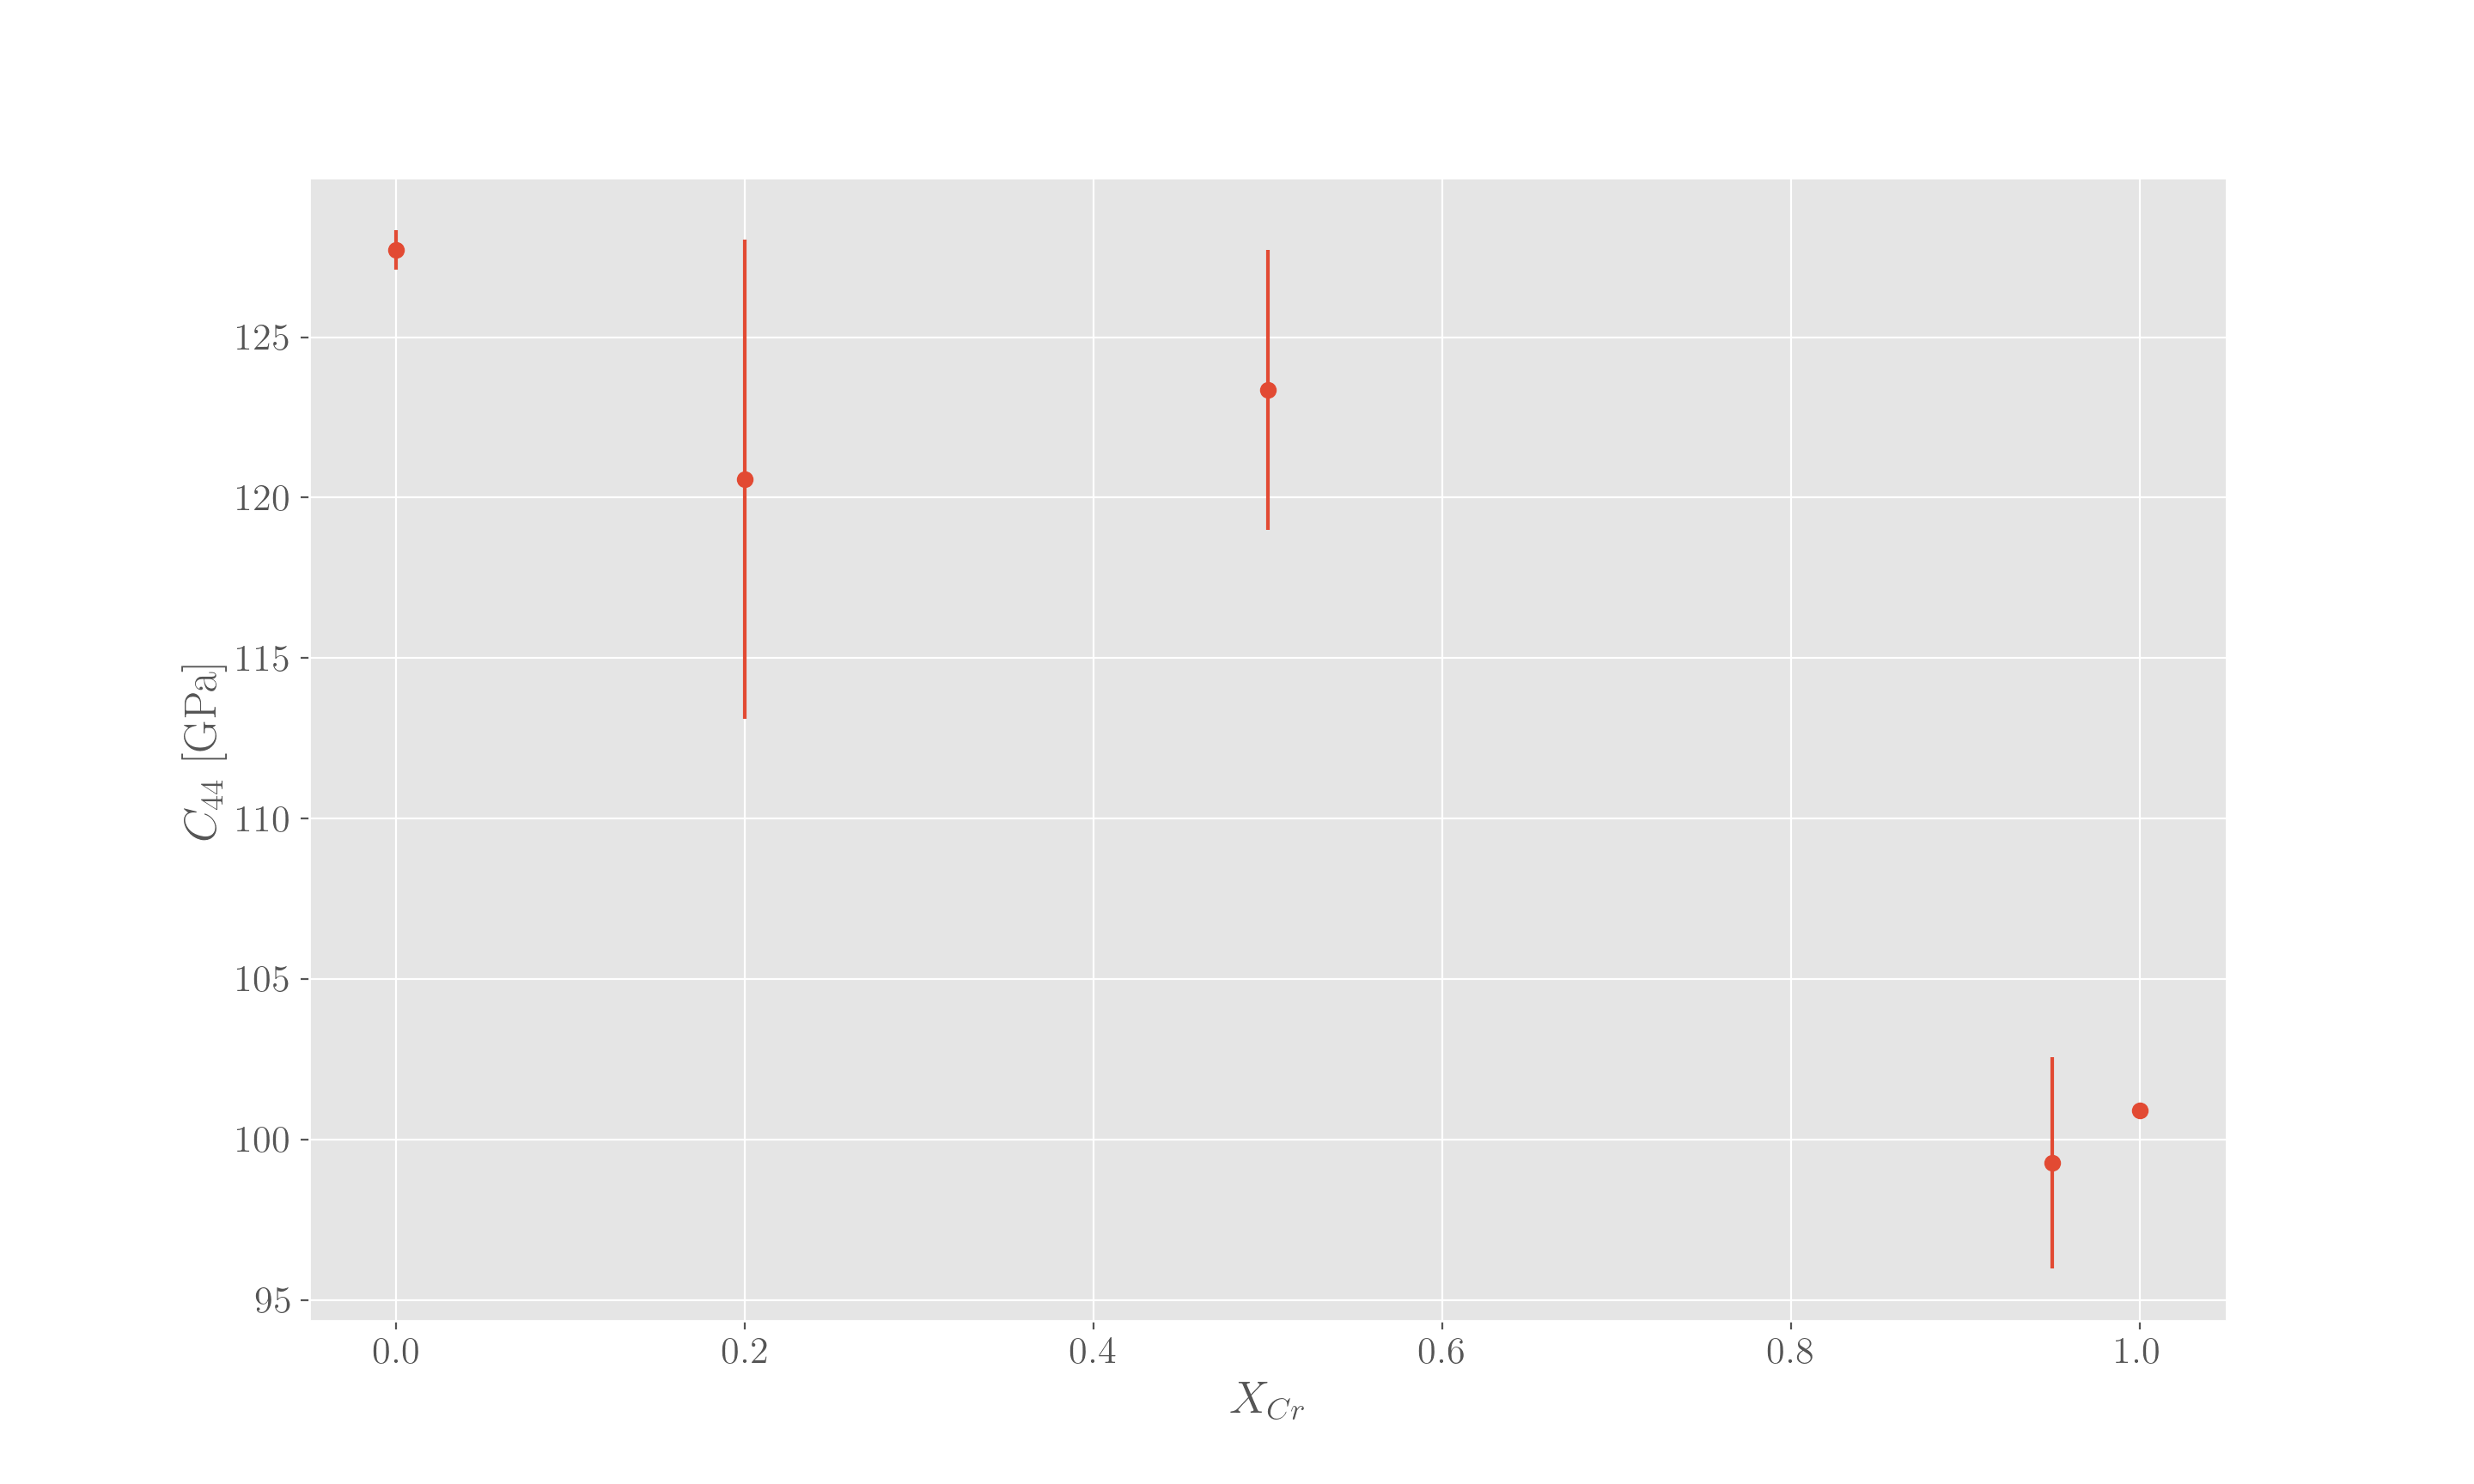
\includegraphics[width=\linewidth]{Parts/Figures/C44.png}
         \caption{Shear constant, \(C_{44}\), representing shear stiffness against deformation without volume change, critical for assessing material's resistance to applied shear stress.}
         \label{fig1c}
     \end{subfigure}
	\caption{Elastic constants of \DIFaddbeginFL \DIFaddFL{homogeneous }\DIFaddendFL bcc \DIFdelbeginFL \DIFdelFL{binary }\DIFdelendFL FeCr \DIFaddbeginFL \DIFaddFL{from the present DFT calculations (40-atom SQS) }\DIFaddendFL as a function of Cr composition\DIFdelbeginFL \DIFdelFL{indicate spinodal decomposition-induced stiffening towards embrittlement}\DIFdelendFL . \DIFdelbeginFL \DIFdelFL{The trends and values are consistent with theoretical and experimental results reported in literature. }\DIFdelendFL (a) Shows the longitudinal stiffness parameter \(C_{11}\), important for evaluating the material's response to compressive and tensile stresses. (b) Highlights \(C_{12}\), which is essential for understanding the coupling between different types of strain. (c) Details \(C_{44}\), crucial for evaluating the shear deformation behavior.}
	\label{fig1}
\end{figure}


\begin{figure}[!ht]
	\centering
	\begin{subfigure}{0.9\textwidth}
         \centering
         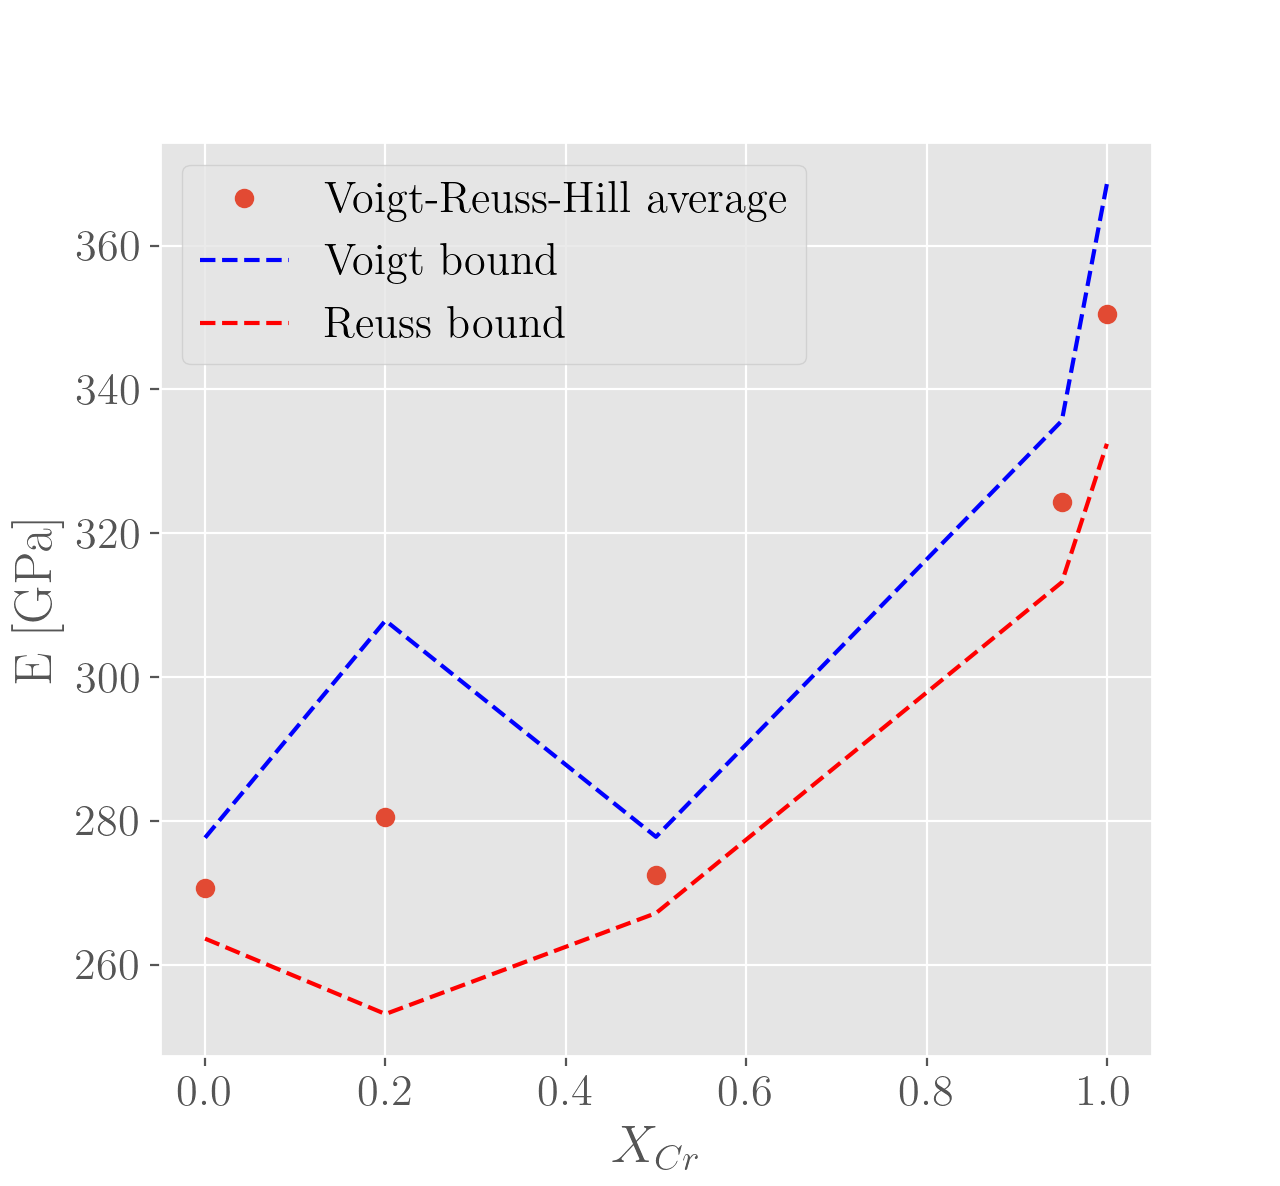
\includegraphics[width=0.9\linewidth]{Parts/Figures/E_VRH.png}
         \caption{Elastic (Young's) Modulus, \(E_{VRH}\), indicating the material's stiffness and its ability to resist deformation under tensile stress.}
         \label{fig2a}
     \end{subfigure}
     \hfill
     \begin{subfigure}{0.45\textwidth}
         \centering
         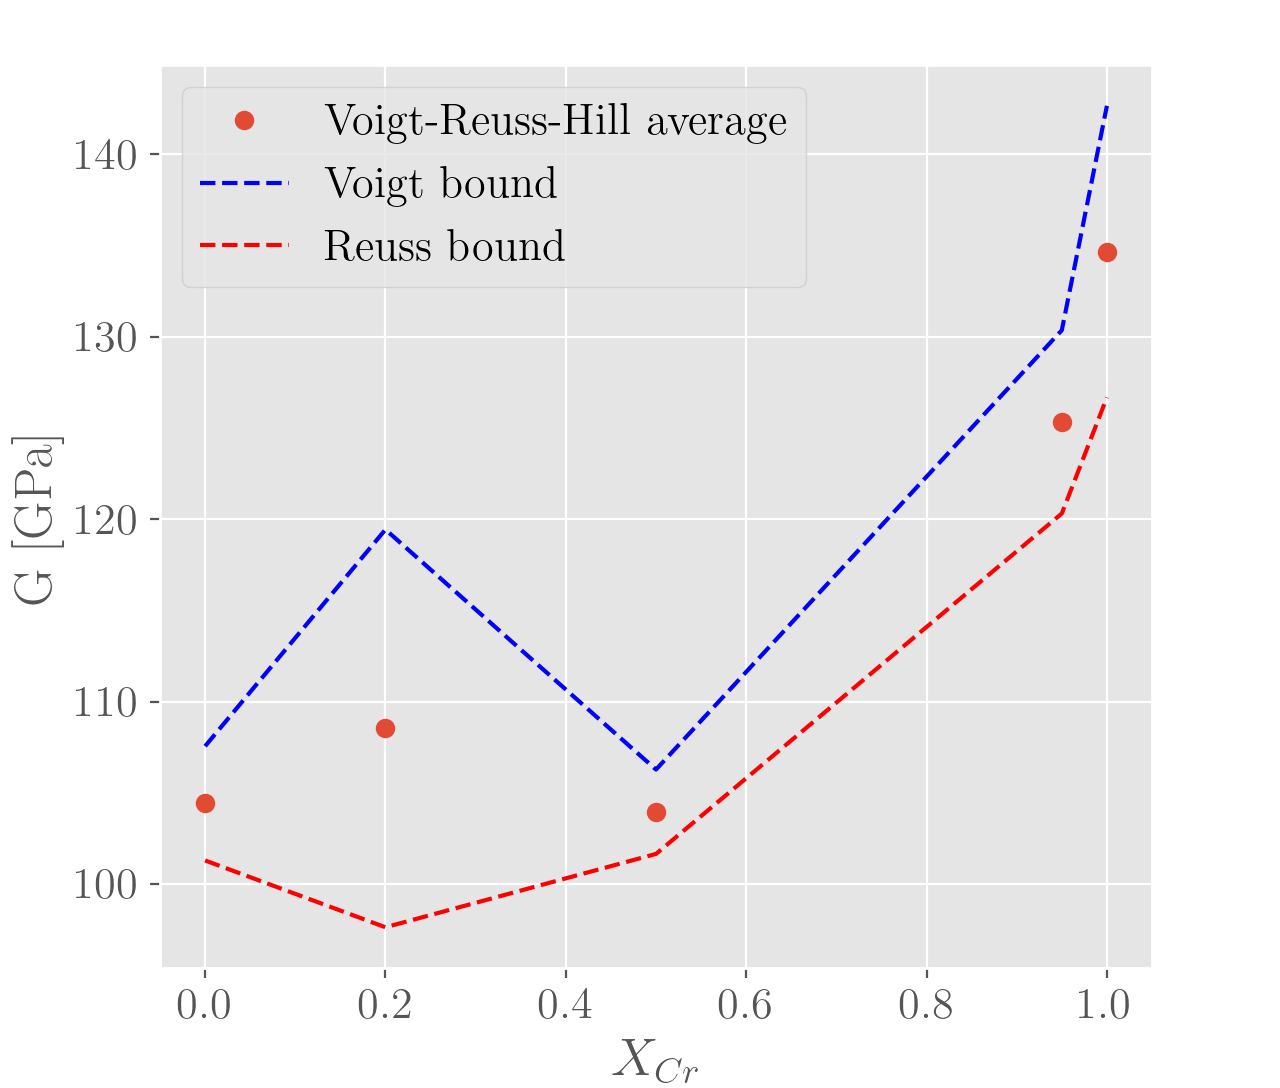
\includegraphics[width=\linewidth]{Parts/Figures/G_VRH.png}
         \caption{Shear modulus, \(G_{VRH}\), reflecting the material's ability to withstand shear deformation.}
         \label{fig2b}
     \end{subfigure}
     \hfill
     \begin{subfigure}{0.45\textwidth}
         \centering
         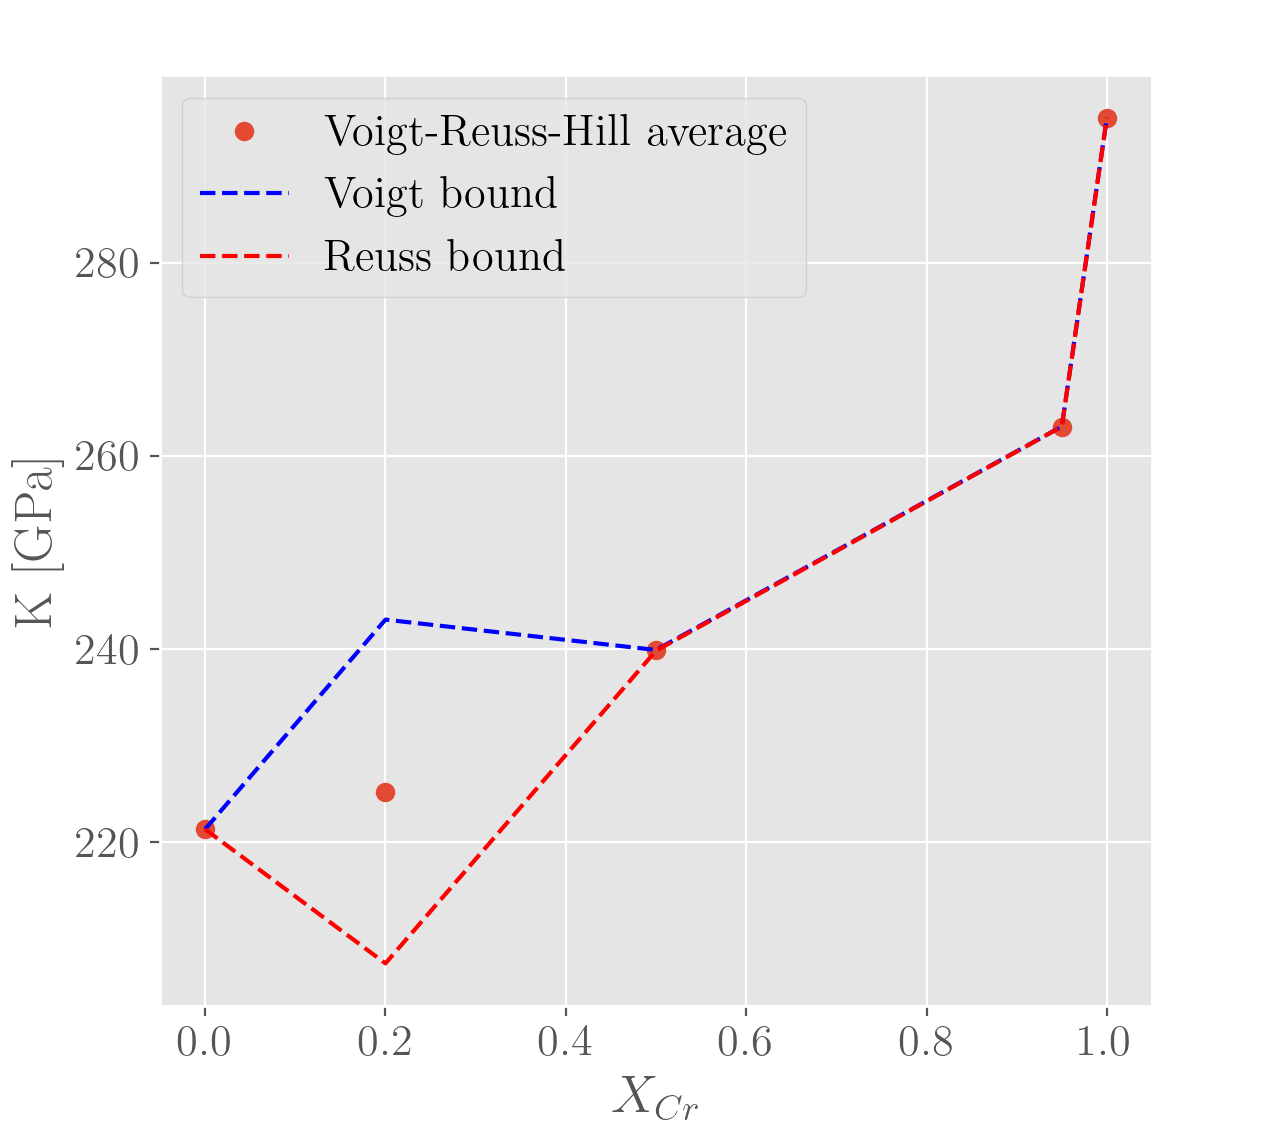
\includegraphics[width=\linewidth]{Parts/Figures/K_VRH.png}
         \caption{Bulk modulus, \(K_{VRH}\), which measures the material's resistance to uniform compression.}
         \label{fig2c}
     \end{subfigure}
	\caption{\DIFdelbeginFL \DIFdelFL{Elastic }\DIFdelendFL \DIFaddbeginFL \DIFaddFL{VRH elastic }\DIFaddendFL moduli of \DIFaddbeginFL \DIFaddFL{homogeneous }\DIFaddendFL bcc \DIFdelbeginFL \DIFdelFL{binary }\DIFdelendFL FeCr \DIFaddbeginFL \DIFaddFL{from the present DFT calculations }\DIFaddendFL as a function of Cr composition\DIFdelbeginFL \DIFdelFL{indicate spinodal decomposition-induced stiffening towards embrittlement}\DIFdelendFL . \DIFdelbeginFL \DIFdelFL{The trends and values are consistent with theoretical and experimental results reported in literature. }\DIFdelendFL (a) Elastic (Young's) Modulus demonstrates the material's overall stiffness. (b) Shear modulus is a measure of the alloy's rigidity against shear forces. (c) Bulk modulus assesses the material's compressibility under uniform pressure.}
	\label{fig2}
\end{figure}

\begin{sidewaysfigure}[!ht]
	\centering
	\begin{subfigure}{0.7\textwidth}
         \centering
         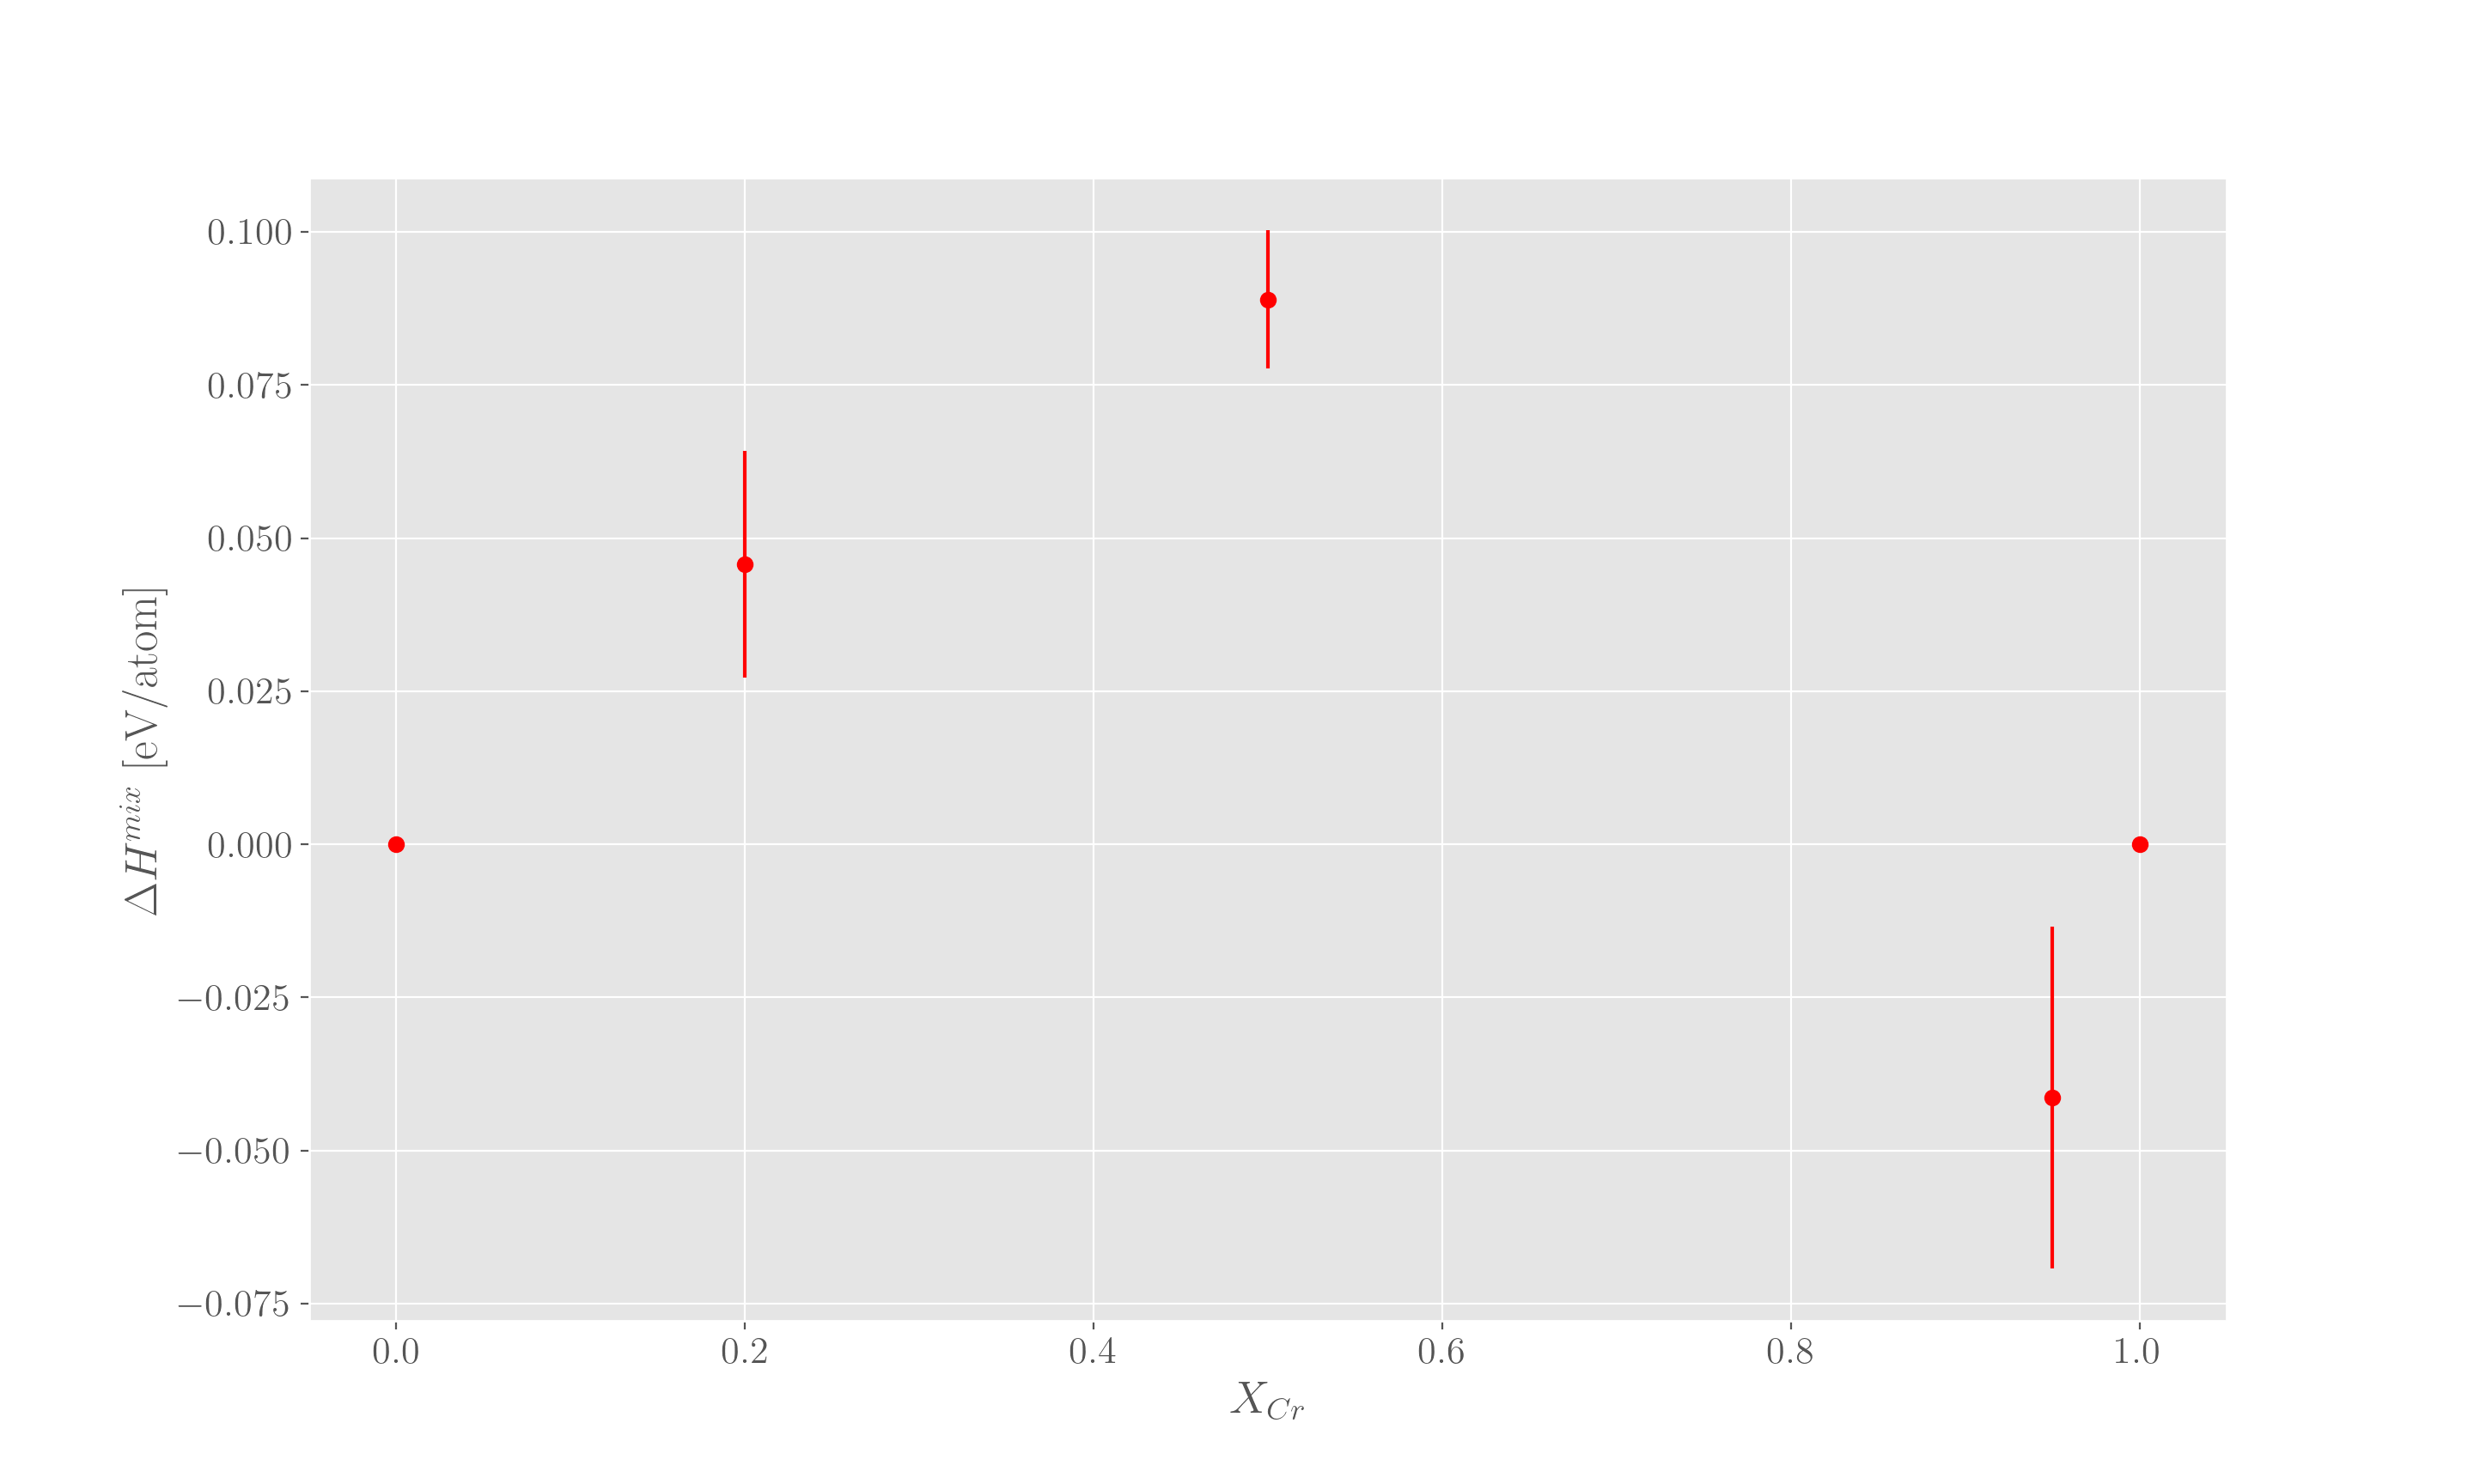
\includegraphics[width=\linewidth]{Parts/Figures/Hmix-vF.png}
         \caption{Enthalpy of mixing, showing the thermodynamic favorability of phase separation in bcc $\delta$-ferrite in cast austenitic stainless steels through spinodal decomposition.}
         \label{fig3a}
     \end{subfigure}
     \begin{subfigure}{0.3\textwidth}
         \centering
         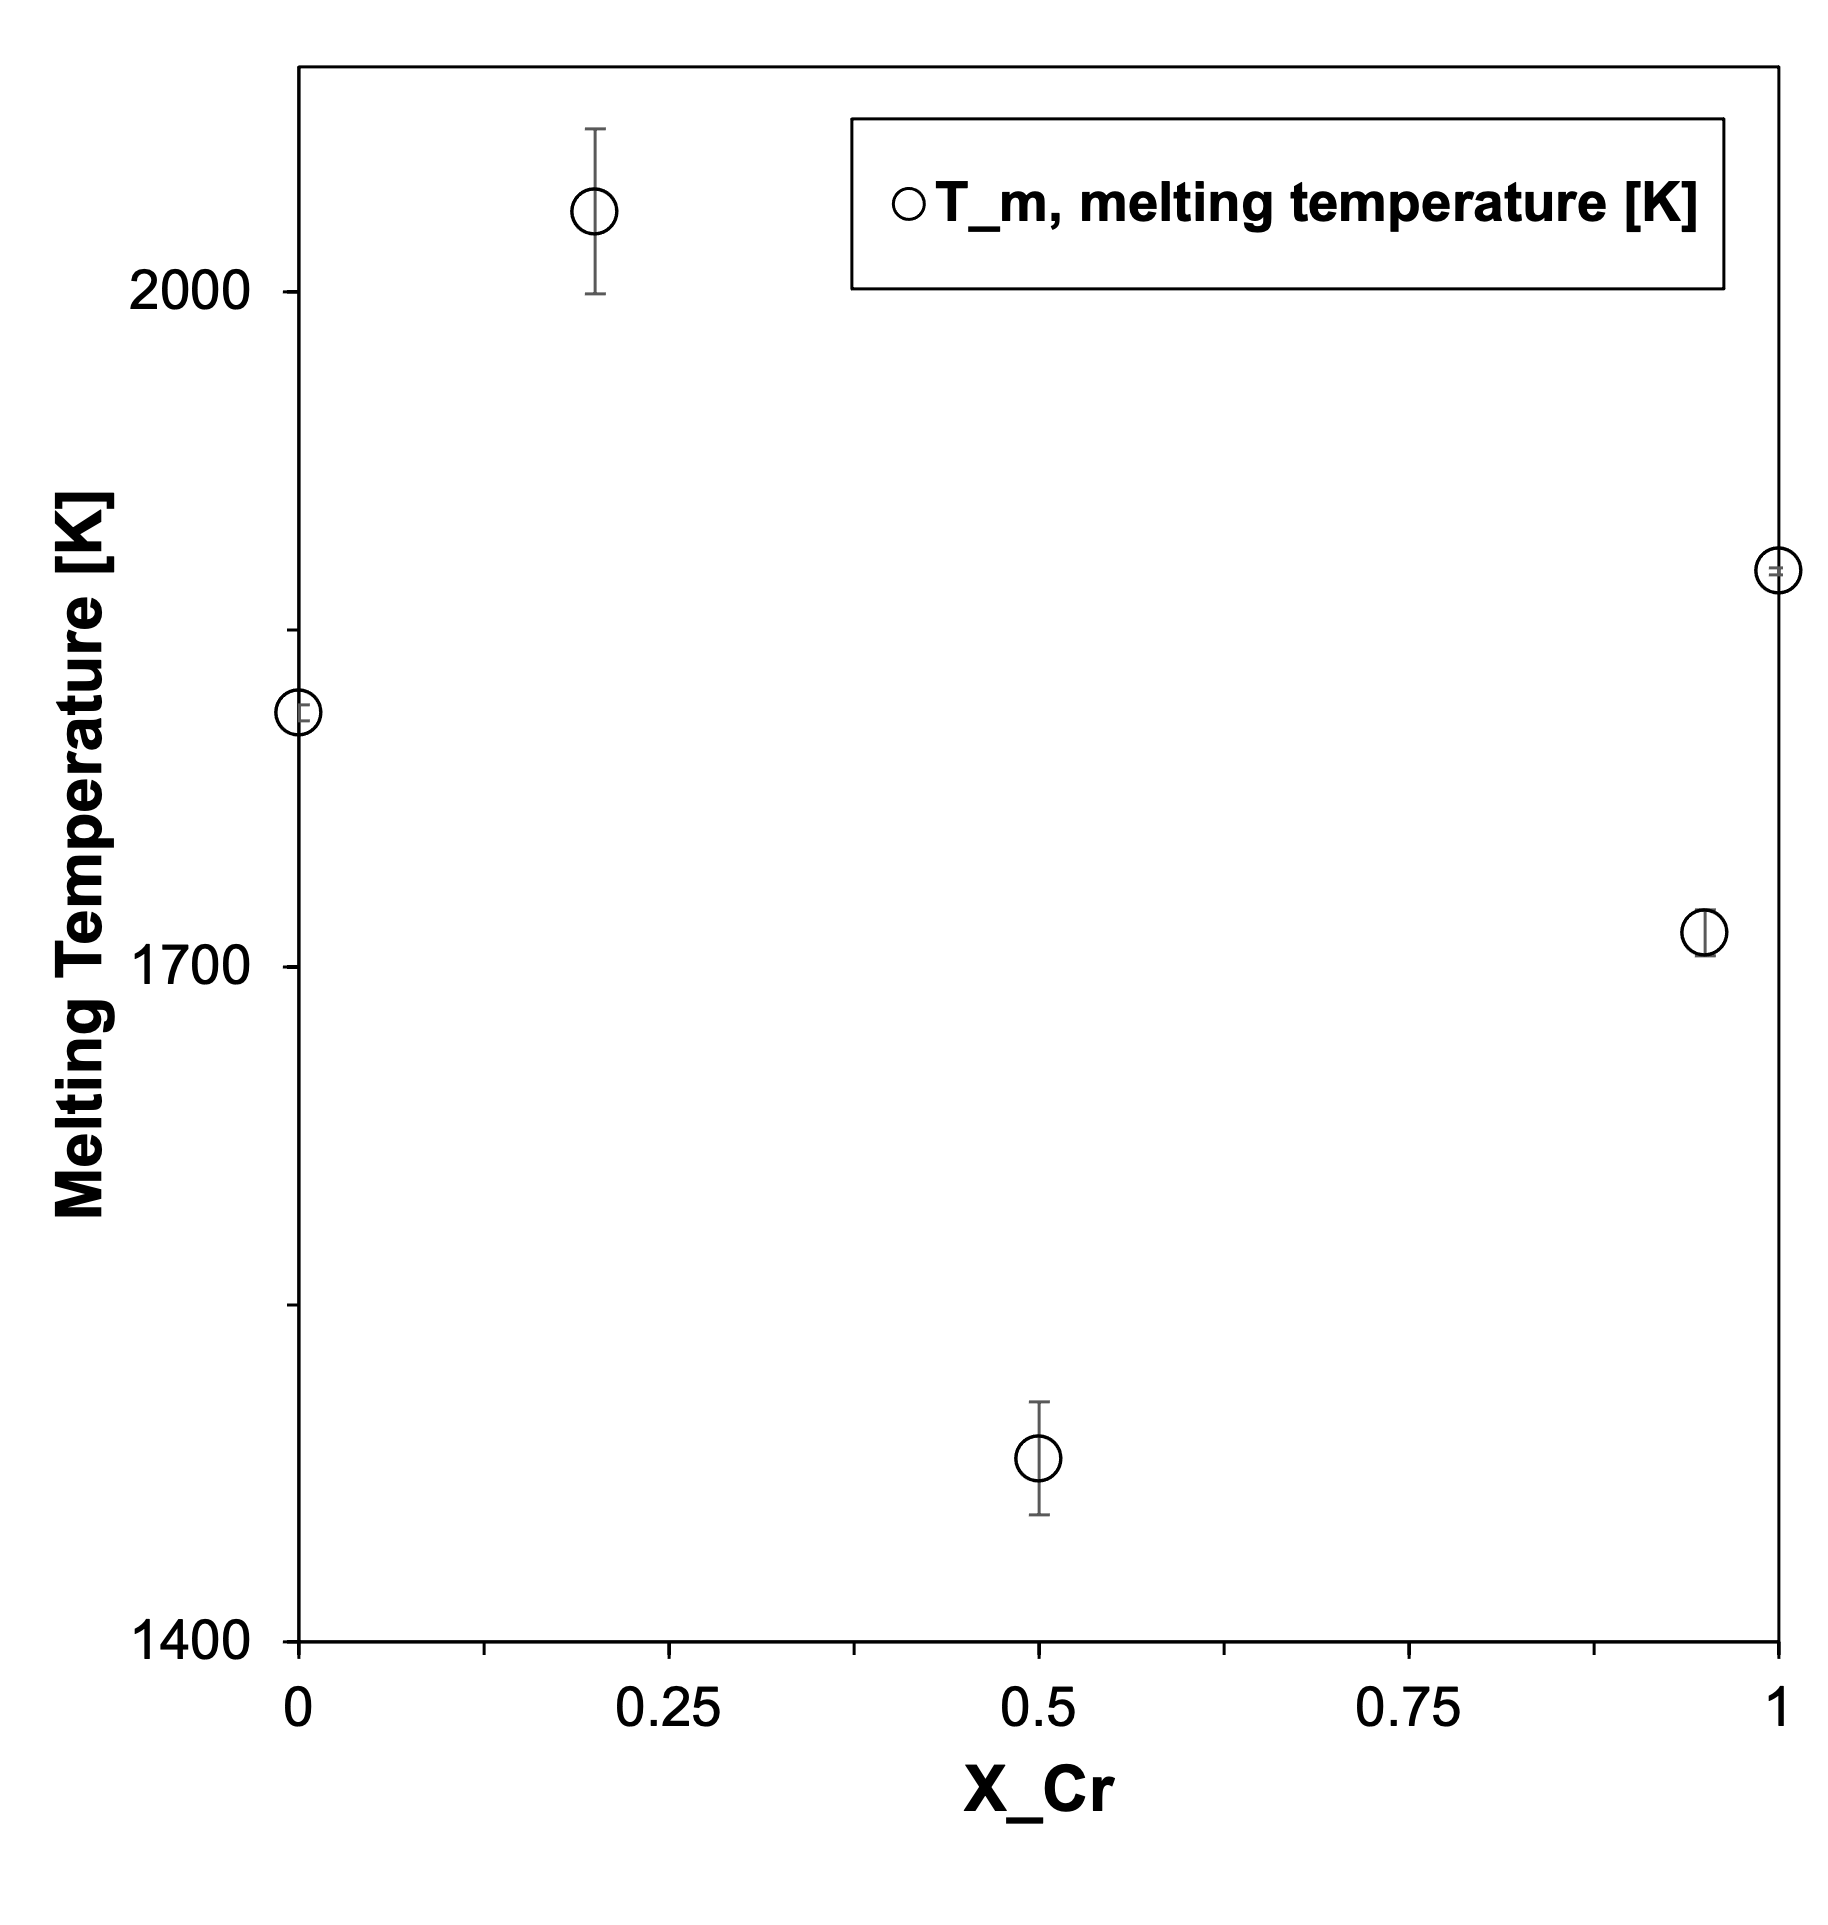
\includegraphics[width=\linewidth]{Parts/Figures/TMvsX_v2.png}
         \caption{\(T_M\), melting temperature, indicating how the thermal stability of the material changes with Cr composition.}
         \label{fig3b}
     \end{subfigure}
     \begin{subfigure}{0.3\textwidth}
         \centering
         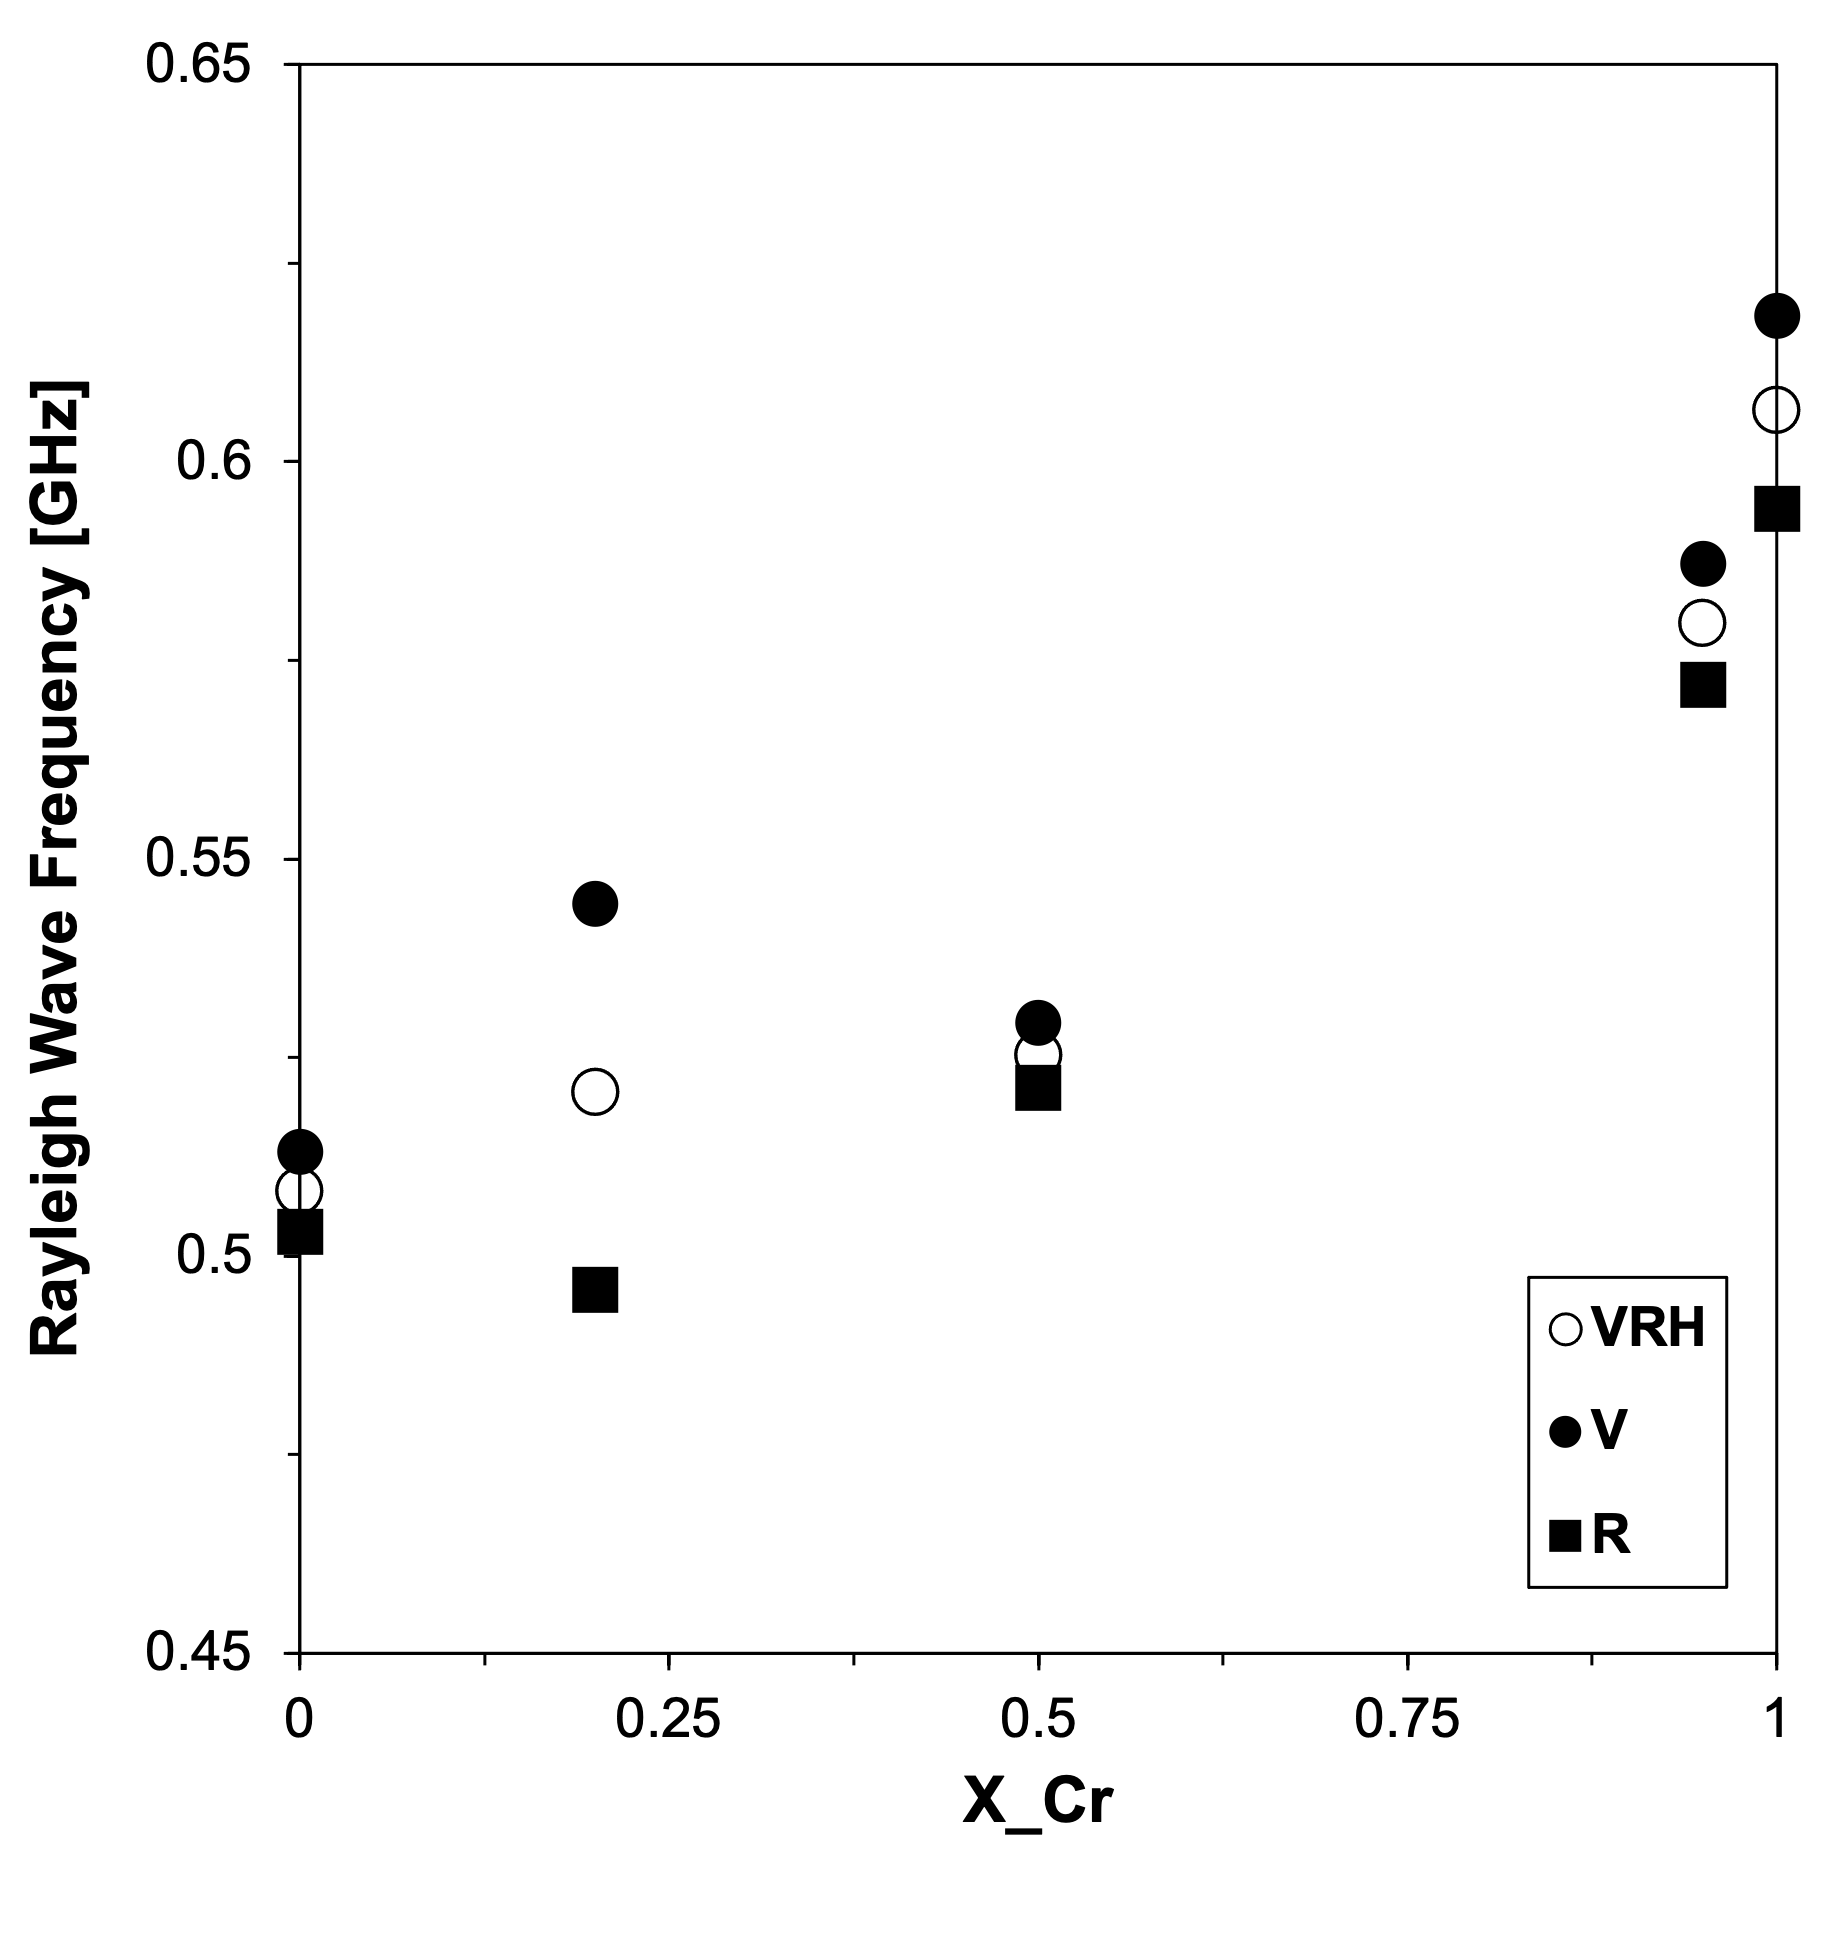
\includegraphics[width=\linewidth]{Parts/Figures/f_rwVsX_vF.png}
         \caption{Rayleigh wave frequencies, illustrating the impact of spinodal decomposition on the material's surface acoustic properties.}
         \label{fig3c}
     \end{subfigure}
     \begin{subfigure}{0.3\textwidth}
         \centering
         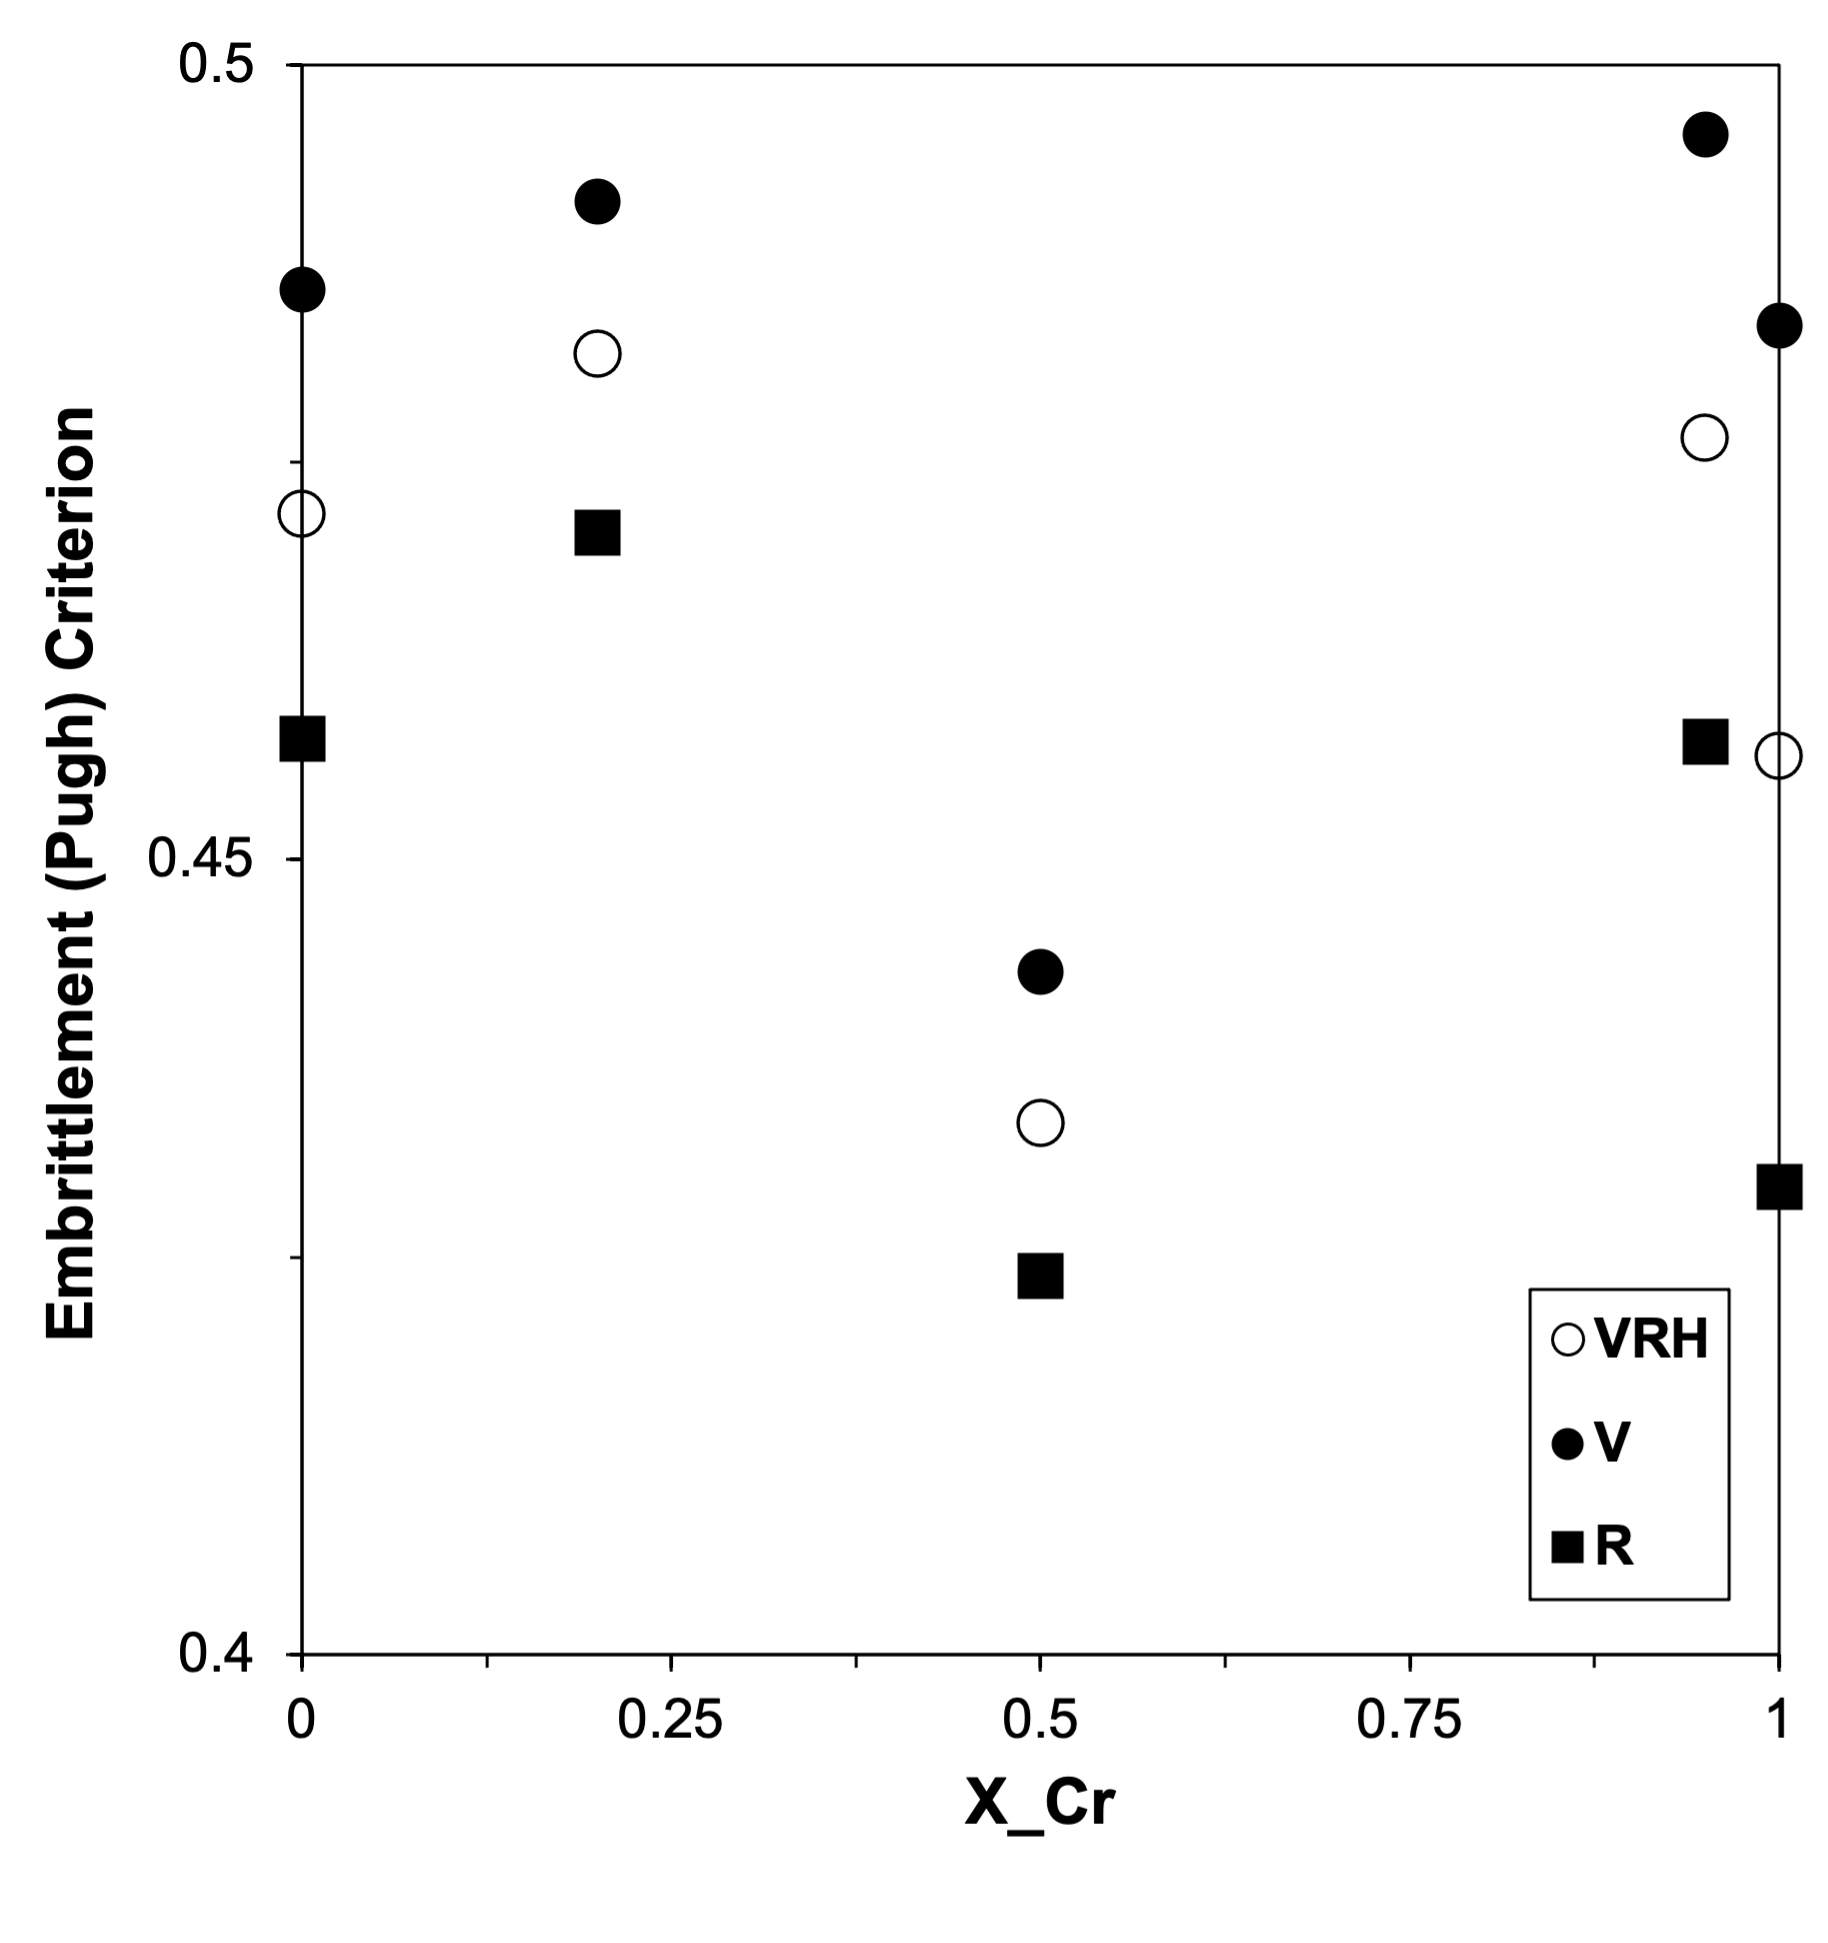
\includegraphics[width=\linewidth]{Parts/Figures/EvsX_vF.png}
         \caption{Embrittlement (Pugh) Criterion, calculated to evaluate the embrittlement risk associated with varying Cr compositions.}
         \label{fig3d}
     \end{subfigure}
	\caption{(a) The enthalpy of mixing demonstrates the thermodynamic drive towards phase separation indicative of spinodal decomposition, affecting the material's mechanical integrity. (b) Variations in the melting temperature as a function of Cr composition offer insights into the thermal stability and potential phase transformations within the alloy. (c) Changes in Rayleigh wave frequencies across compositions highlight alterations in surface acoustic properties, correlating with mechanical behavior. (d) The Embrittlement (Pugh) Criterion allows for assessing the risk of material embrittlement due to changes in composition, crucial for ensuring material reliability in critical applications.}
	\label{fig3}
\end{sidewaysfigure}


\begin{sidewaysfigure}[!ht]
    \centering
    \begin{subfigure}{0.9\textwidth}
        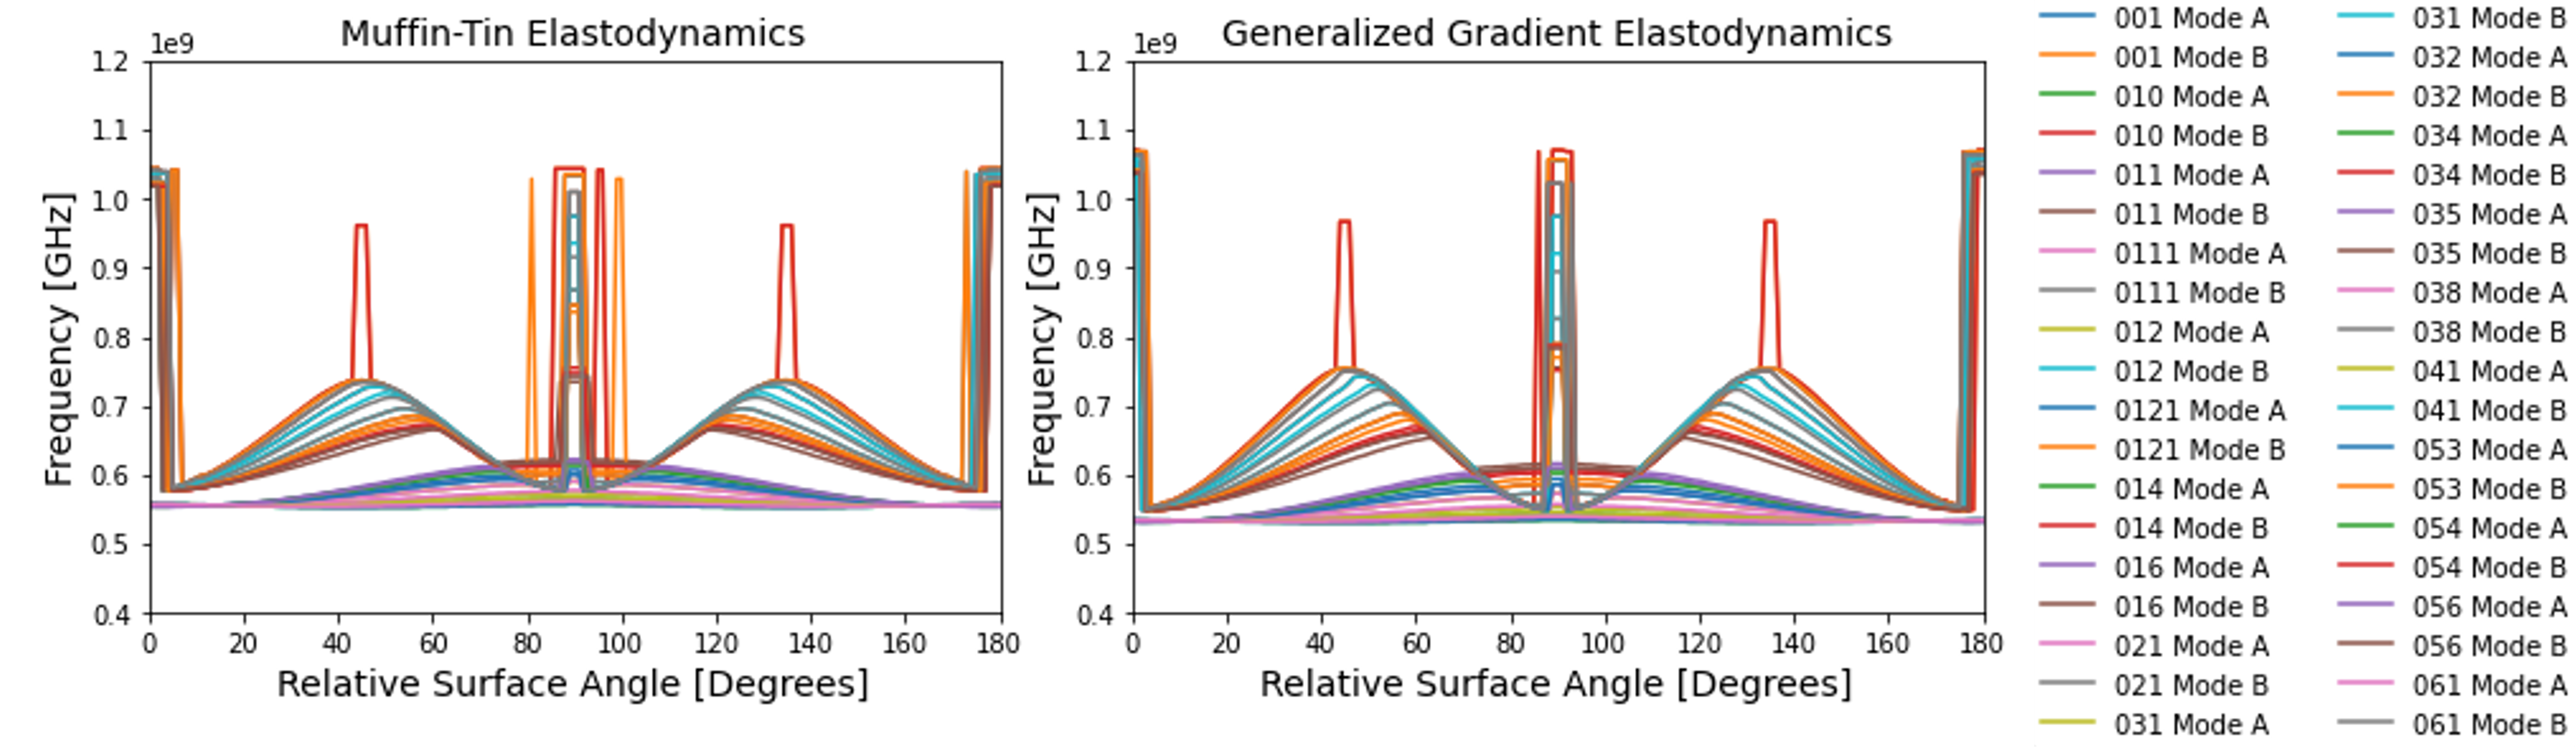
\includegraphics[width=\textwidth]{Parts/Figures/smoking-gun-v2.png}
        \caption{Predicted elastic frequencies showcasing the emergence of new modes within the elastodynamically-unallowed regions, signifying alterations in the material's mechanical properties due to spinodal decomposition.\DIFdelbegin \DIFdel{These frequencies match closely with experimentally observed values in aged stainless steel specimens, providing a quantum mechanical insight into the microstructural evolution impacting material performance.}\DIFdelend }
        \label{fig4a}
    \end{subfigure}
    \begin{subfigure}{0.35\textwidth}
        \DIFdelbegin %DIFDELCMD < 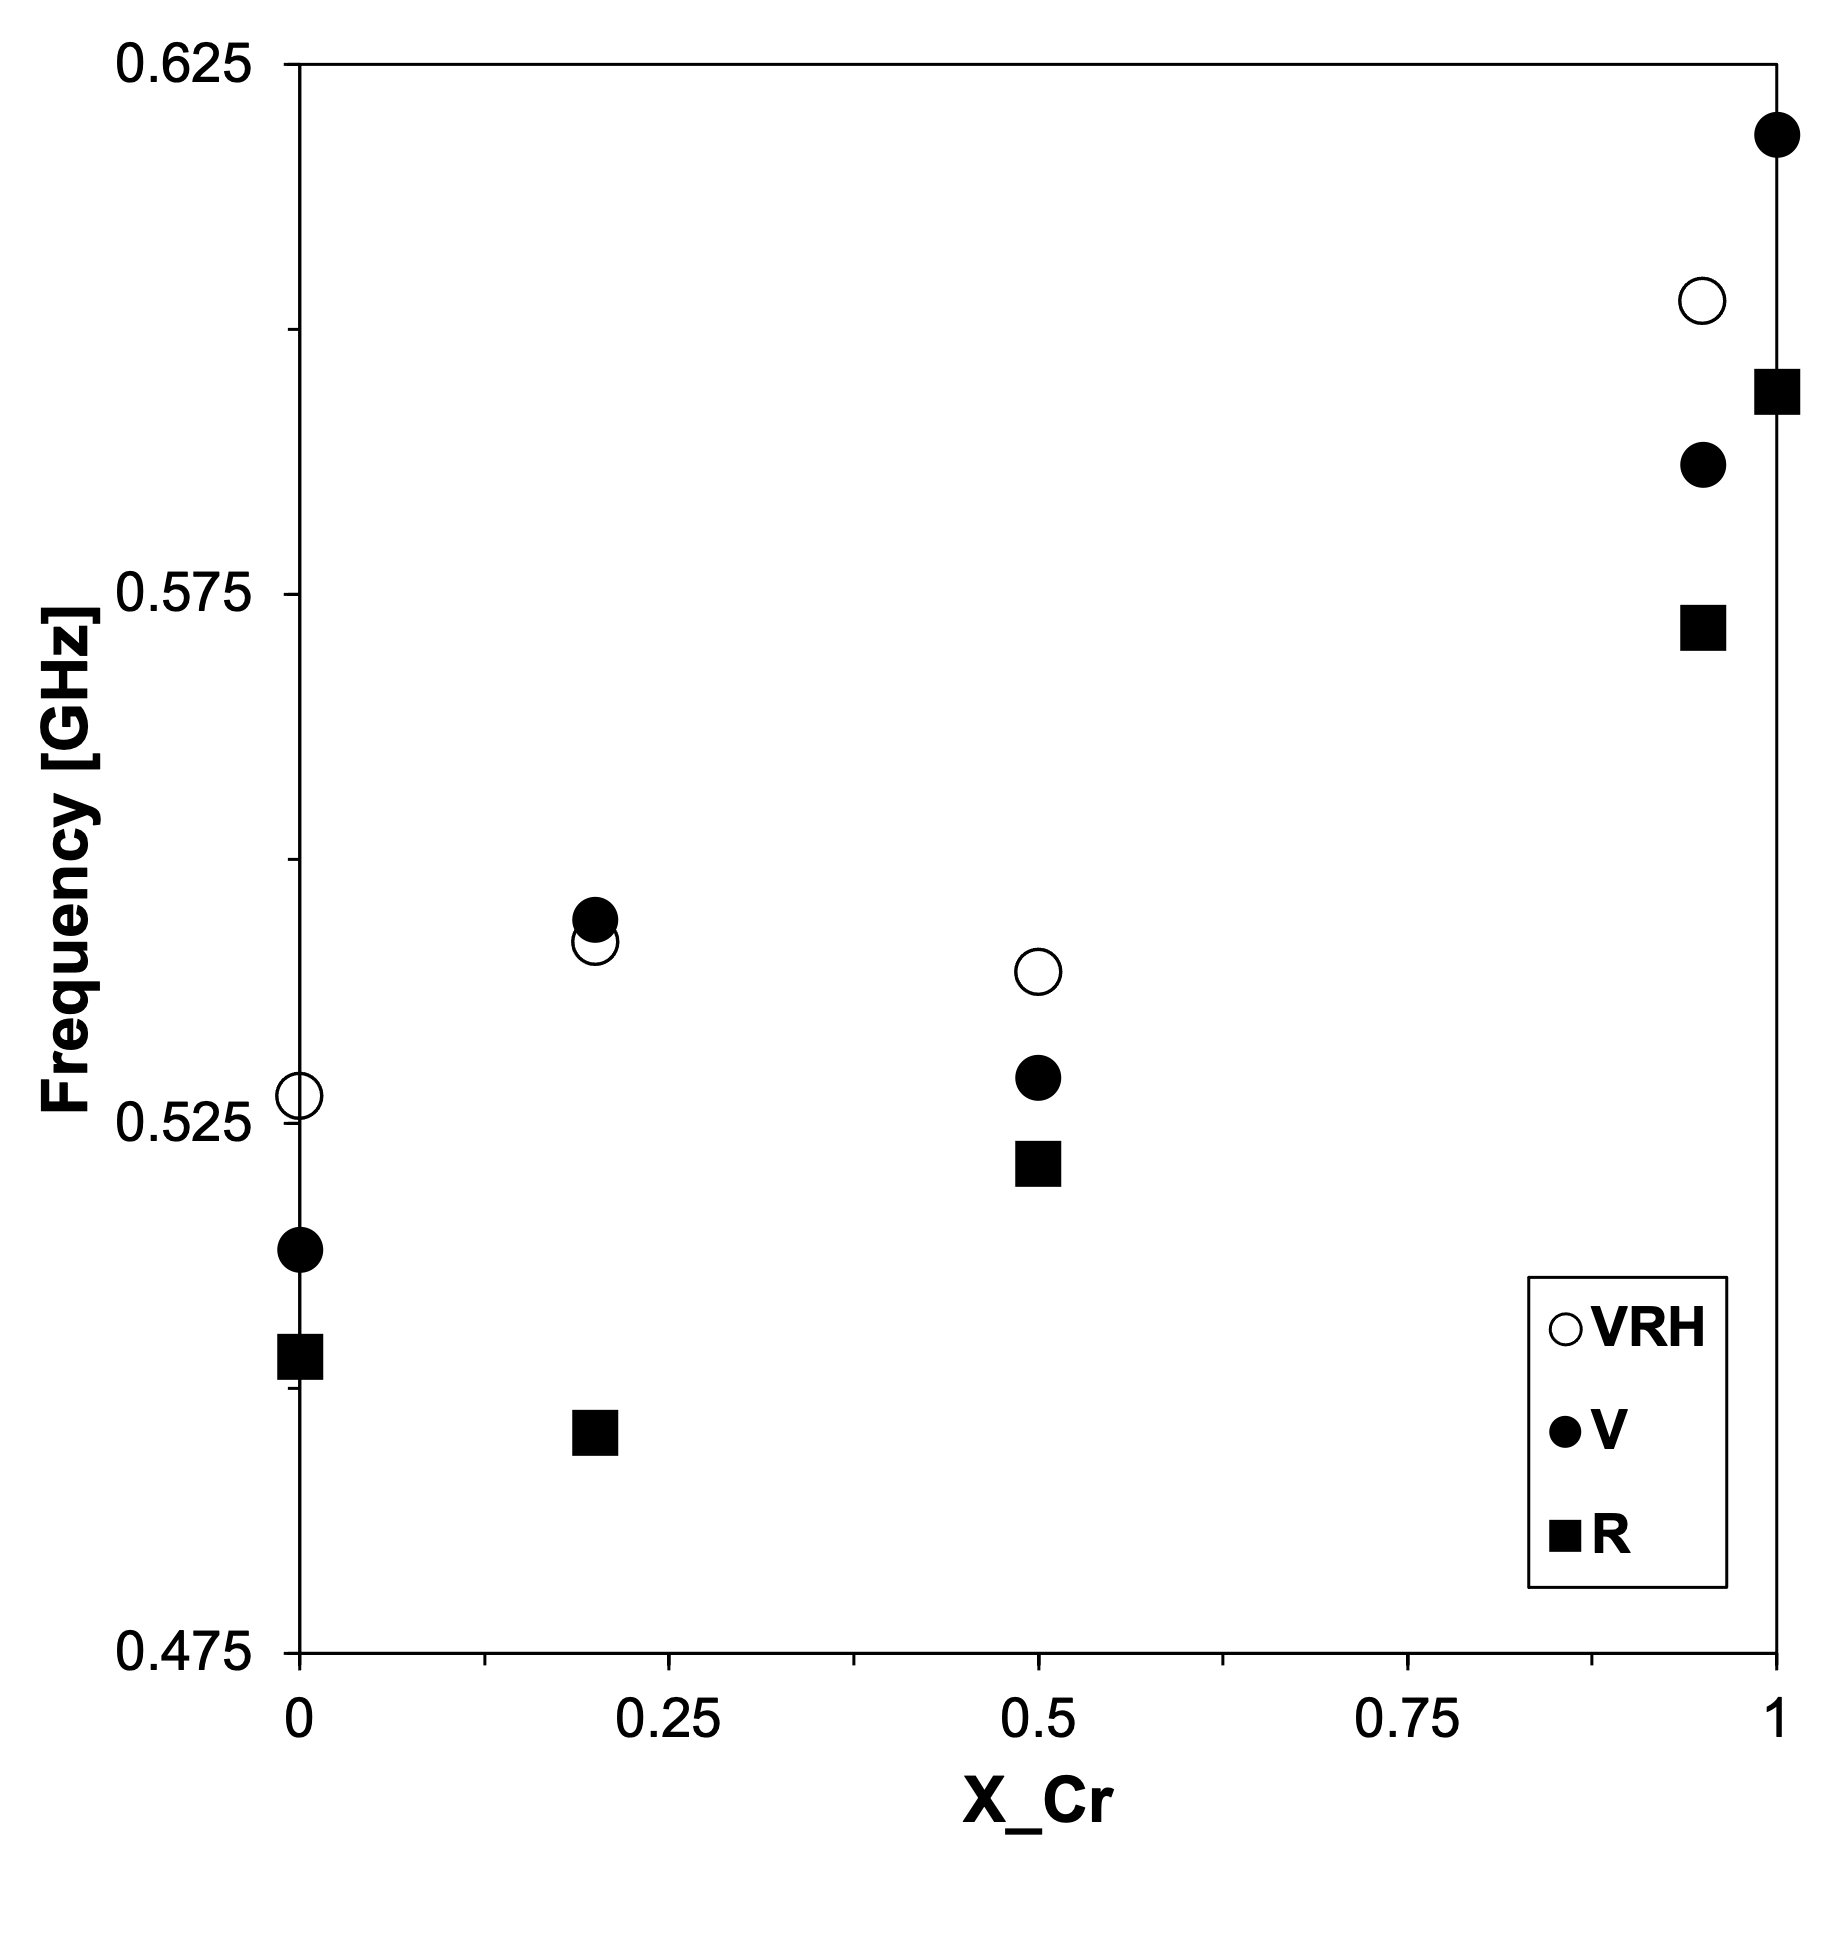
\includegraphics[width=\textwidth, left]{Parts/Figures/fvsX_v3.png}
%DIFDELCMD <         %%%
\DIFdelend \DIFaddbegin 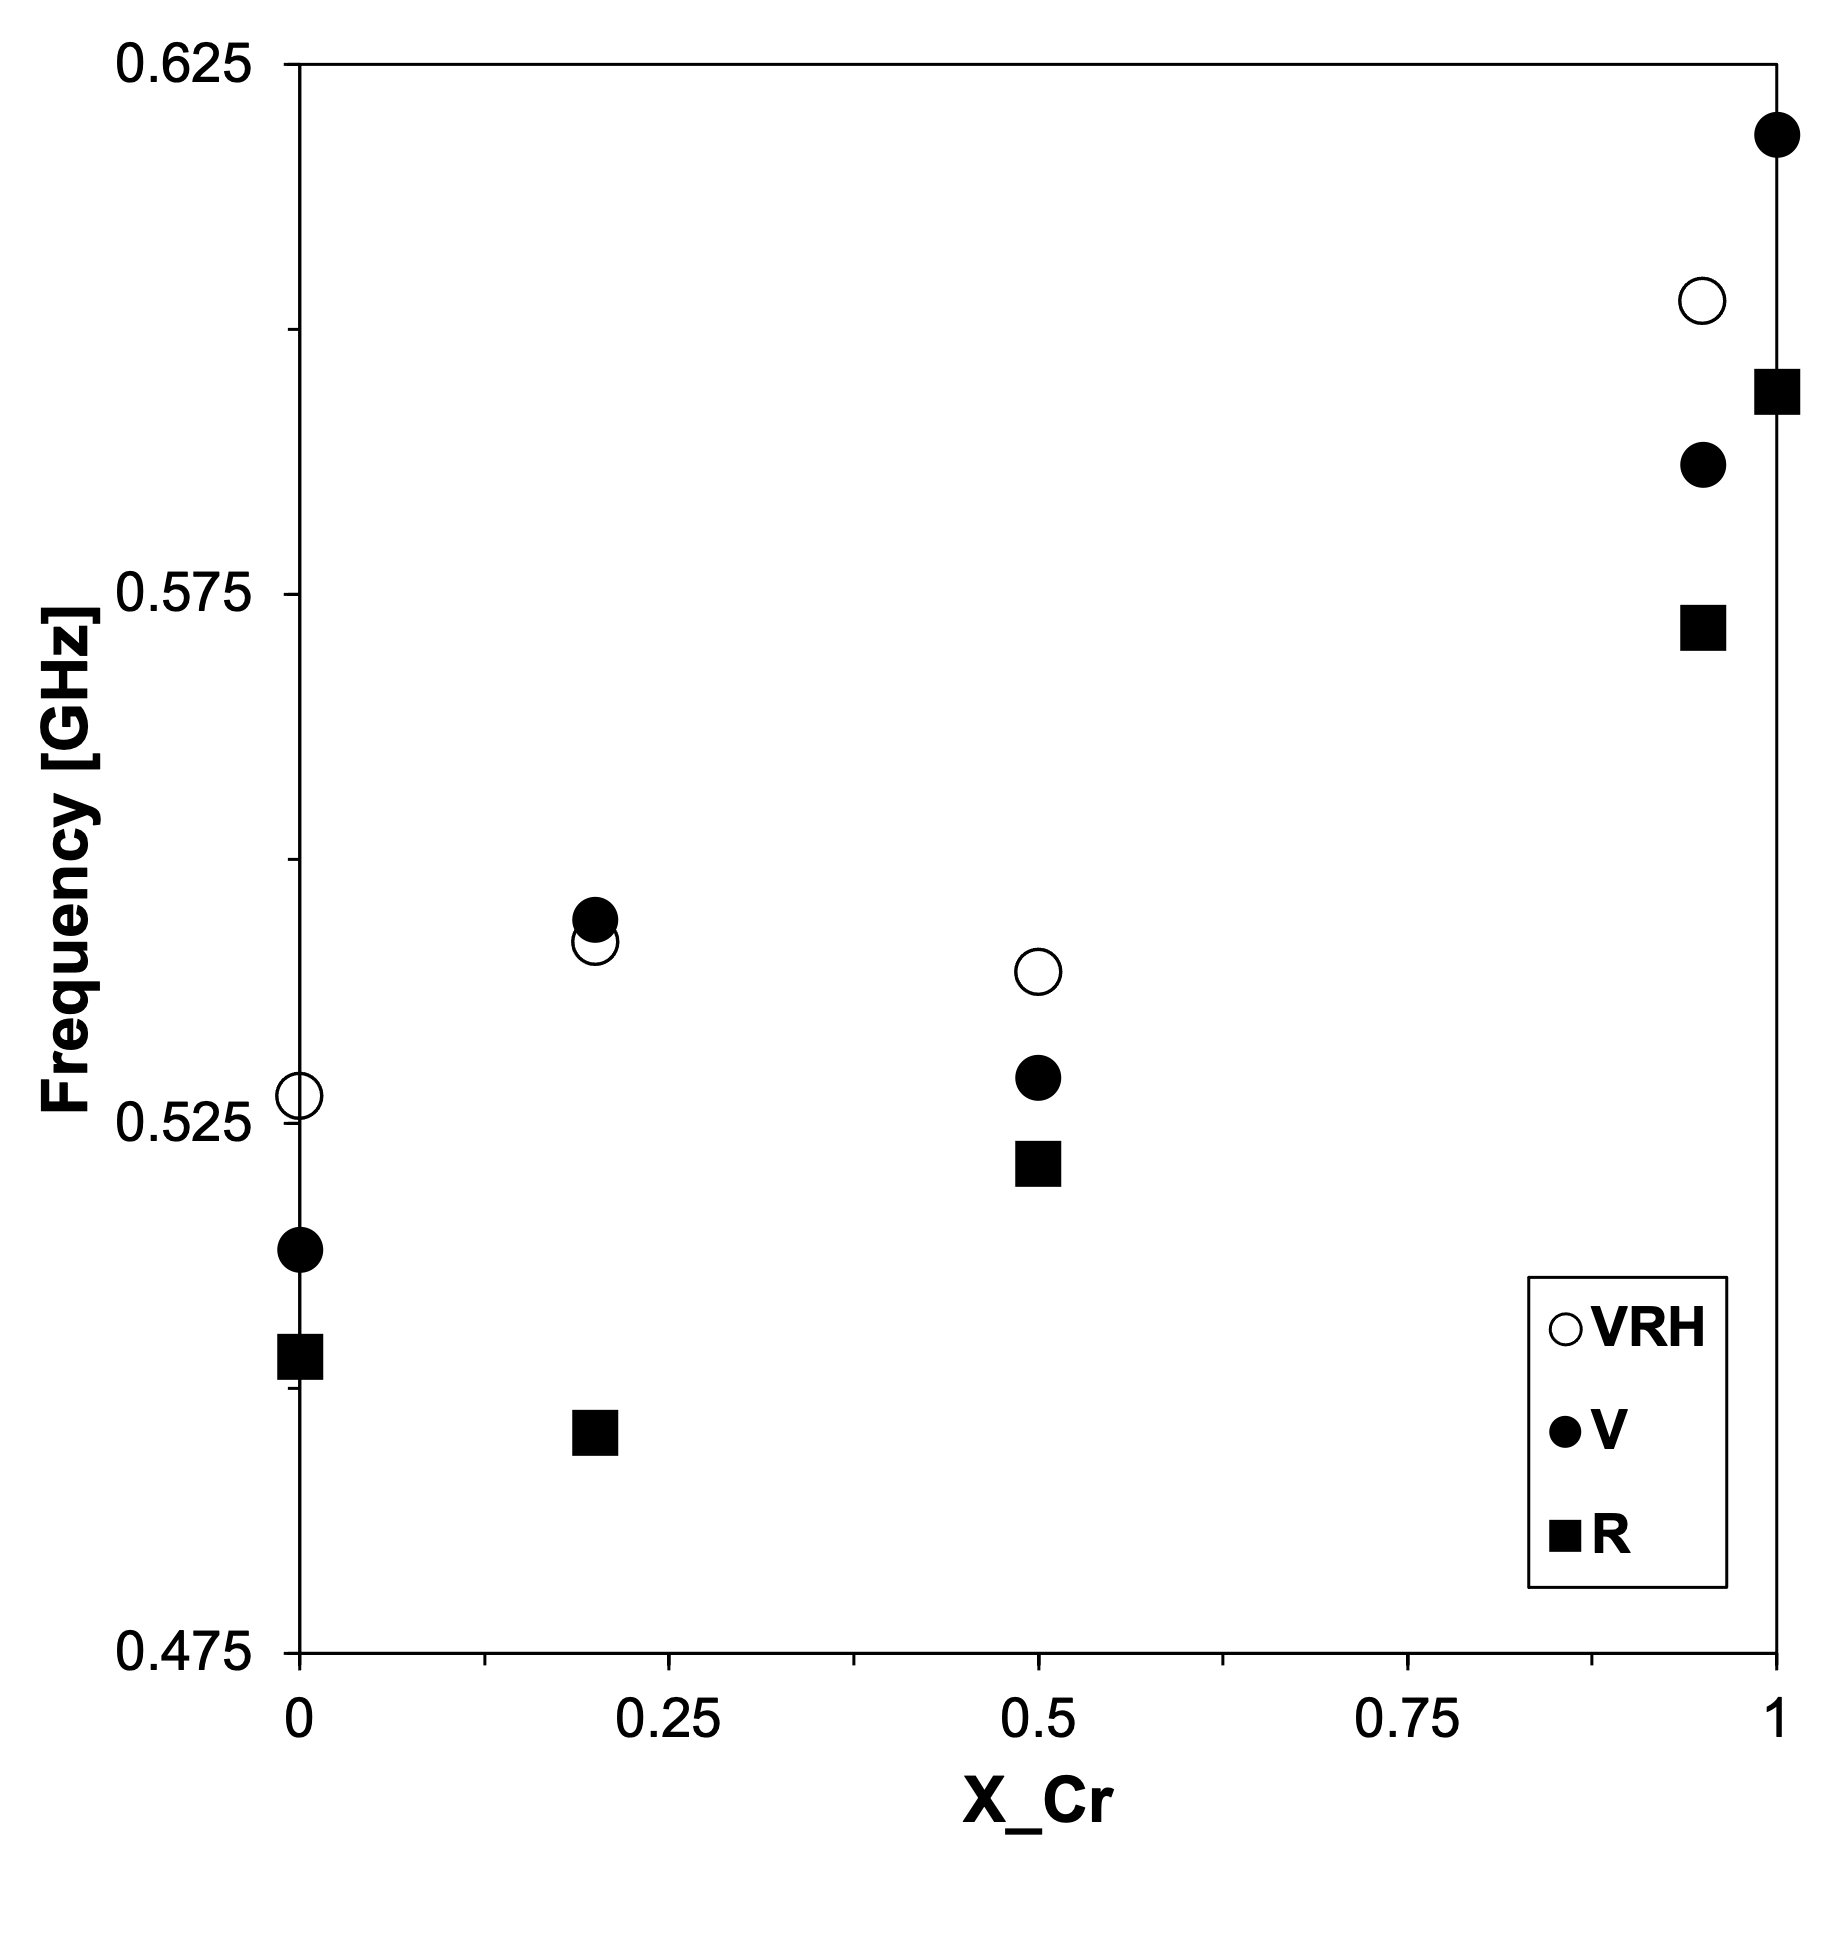
\includegraphics[width=\textwidth]{Parts/Figures/fvsX_v3.png}
        \DIFaddend \caption{Calculated acoustic frequencies across different Cr compositions, illustrating the material's acoustic response variability with composition. This graph provides a quantitative measure of the material's mechanical behavior and its dependence on the microstructural characteristics induced by varying chromium content.}
        \label{fig4b}
    \end{subfigure}
    \begin{subfigure}{0.5\textwidth}
        \DIFdelbegin %DIFDELCMD < 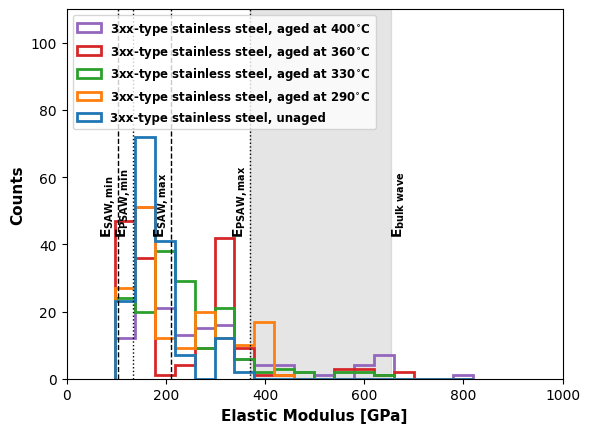
\includegraphics[width=\textwidth, right]{Parts/Figures/experimental-moduli-hist.png}
%DIFDELCMD <         %%%
\DIFdelend \DIFaddbegin 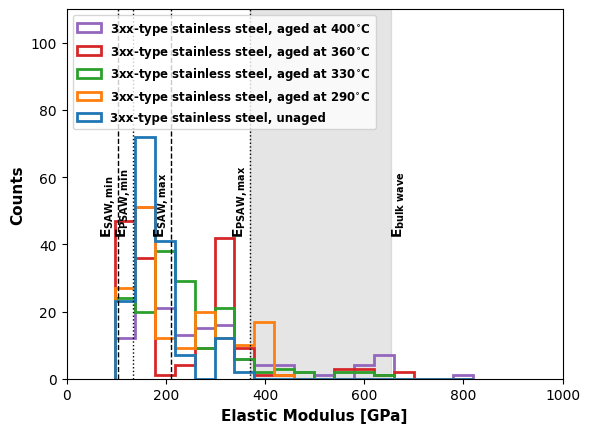
\includegraphics[width=\textwidth]{Parts/Figures/experimental-moduli-hist.png}
        \DIFaddend \caption{Measured elastic moduli distribution from experimental data, highlighting the range and variability of material properties within stainless steel samples subjected to different thermal aging processes. The distribution underscores the significant impact of microstructural changes, such as spinodal decomposition, on the material's overall stiffness and mechanical integrity.}
        \label{fig4c}
    \end{subfigure}
    \caption{(a) Quantum elastodynamic frequencies obtained from density functional theory calculations reveal the complex interplay between microstructural evolution and mechanical properties in stainless steels undergoing spinodal decomposition. These findings are corroborated by (b) calculated acoustic frequencies that vary with Cr composition, providing a link between composition, microstructure, and acoustic properties. (c) The distribution of measured elastic moduli further validates the theoretical predictions, illustrating the broad impact of aging and compositional changes on the material's mechanical performance.}
    \label{fig4}
\end{sidewaysfigure}


\begin{sidewaysfigure}[!ht]
	\centering
	\begin{subfigure}{0.3\textwidth}
         \centering
         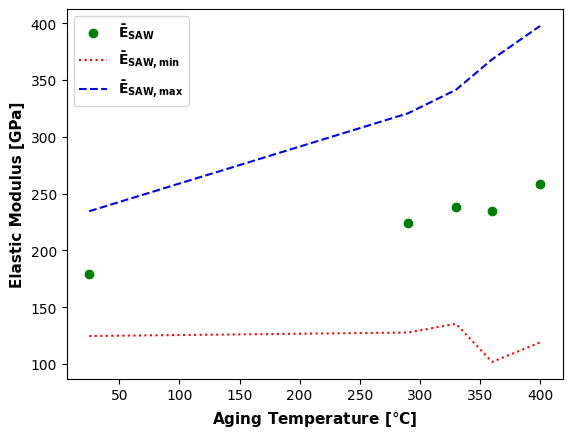
\includegraphics[width=\linewidth]{Parts/Figures/experimental-moduli-trend.png}
         \caption{Experimental elastic moduli of aged steels, displaying how aging temperature influences the material's stiffness. This graph illustrates the correlation between thermal treatment and the increase in elastic moduli, indicative of the material's response to microstructural changes over time.}
         \label{fig5a}
     \end{subfigure}
     \hfill
     \begin{subfigure}{0.3\textwidth}
         \centering
         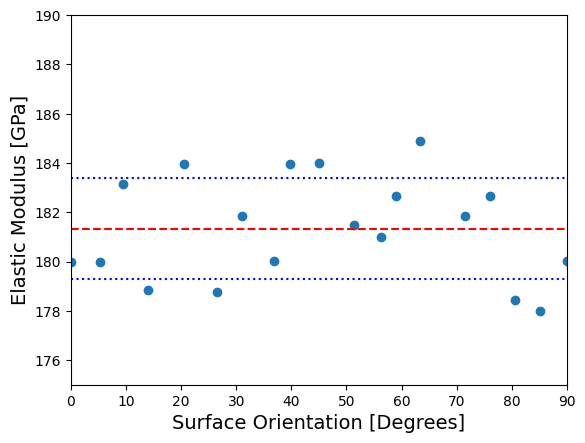
\includegraphics[width=\linewidth]{Parts/Figures/approximate-elastic-moduli-from-SAW-measurements-pristine.png}
         \caption{Theoretical elastic moduli of pristine steels, offering a baseline comparison for understanding how spinodal decomposition affects material properties before and after aging. This comparison elucidates the stiffening effect of microstructural evolution on the alloy's mechanical behavior.}
         \label{fig5b}
     \end{subfigure}
     \hfill
     \begin{subfigure}{0.3\textwidth}
         \centering
         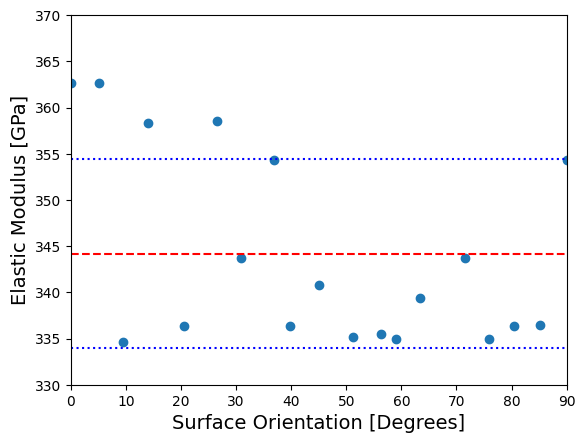
\includegraphics[width=\linewidth]{Parts/Figures/approximate-elastic-moduli-from-SAW-measurements-spindec.png}
         \caption{Theoretical elastic moduli of spinodally decomposed steels, demonstrating the pronounced impact of microstructural evolution on the alloy's stiffness. This direct comparison to pristine conditions highlights the significant role of chromium composition and thermal aging in material performance.}
         \label{fig5c}
     \end{subfigure}
     \hfill
     \begin{subfigure}{0.3\textwidth}
         \centering
         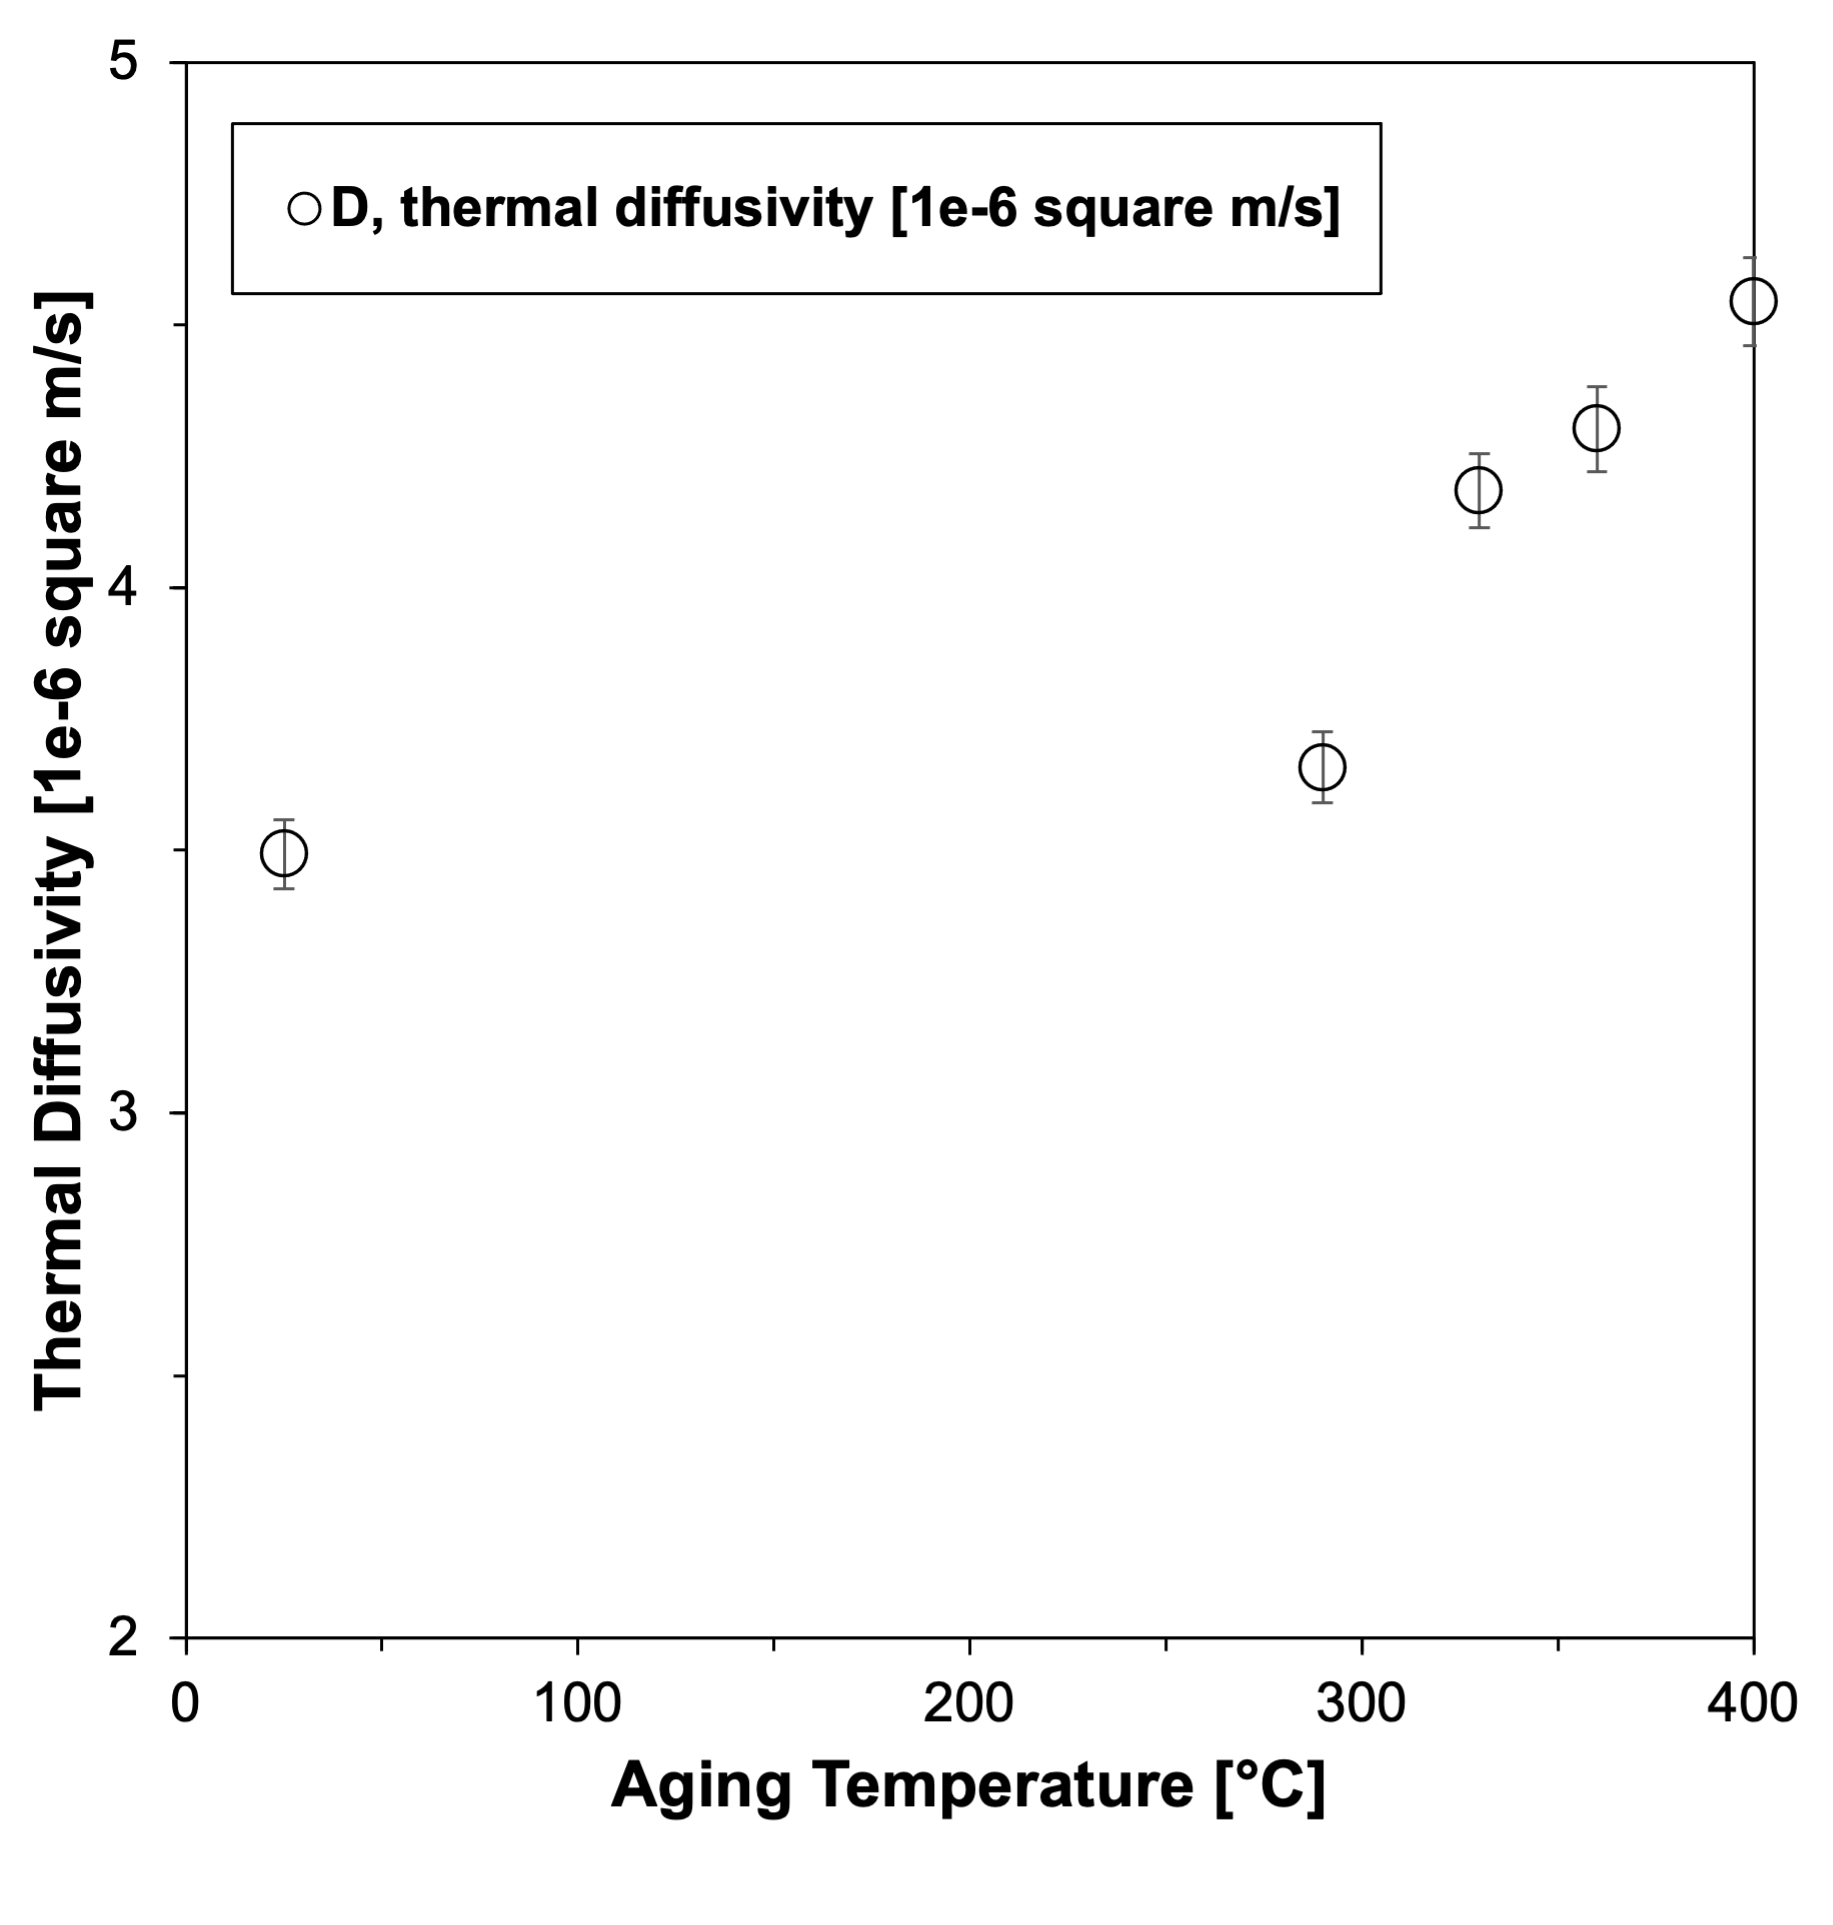
\includegraphics[width=\linewidth]{Parts/Figures/DvsT_CF8_30khrs_v2.png}
         \caption{\(D^{exp}_{thermal}\), experimental thermal diffusivity as measured in aged stainless steel, illustrating the thermal transport characteristics and their variation with temperature. This metric provides insights into the thermal stability and heat dissipation capabilities of the material post-aging.}
         \label{fig5d}
     \end{subfigure}
     \hfill
     \begin{subfigure}{0.3\textwidth}
         \centering
         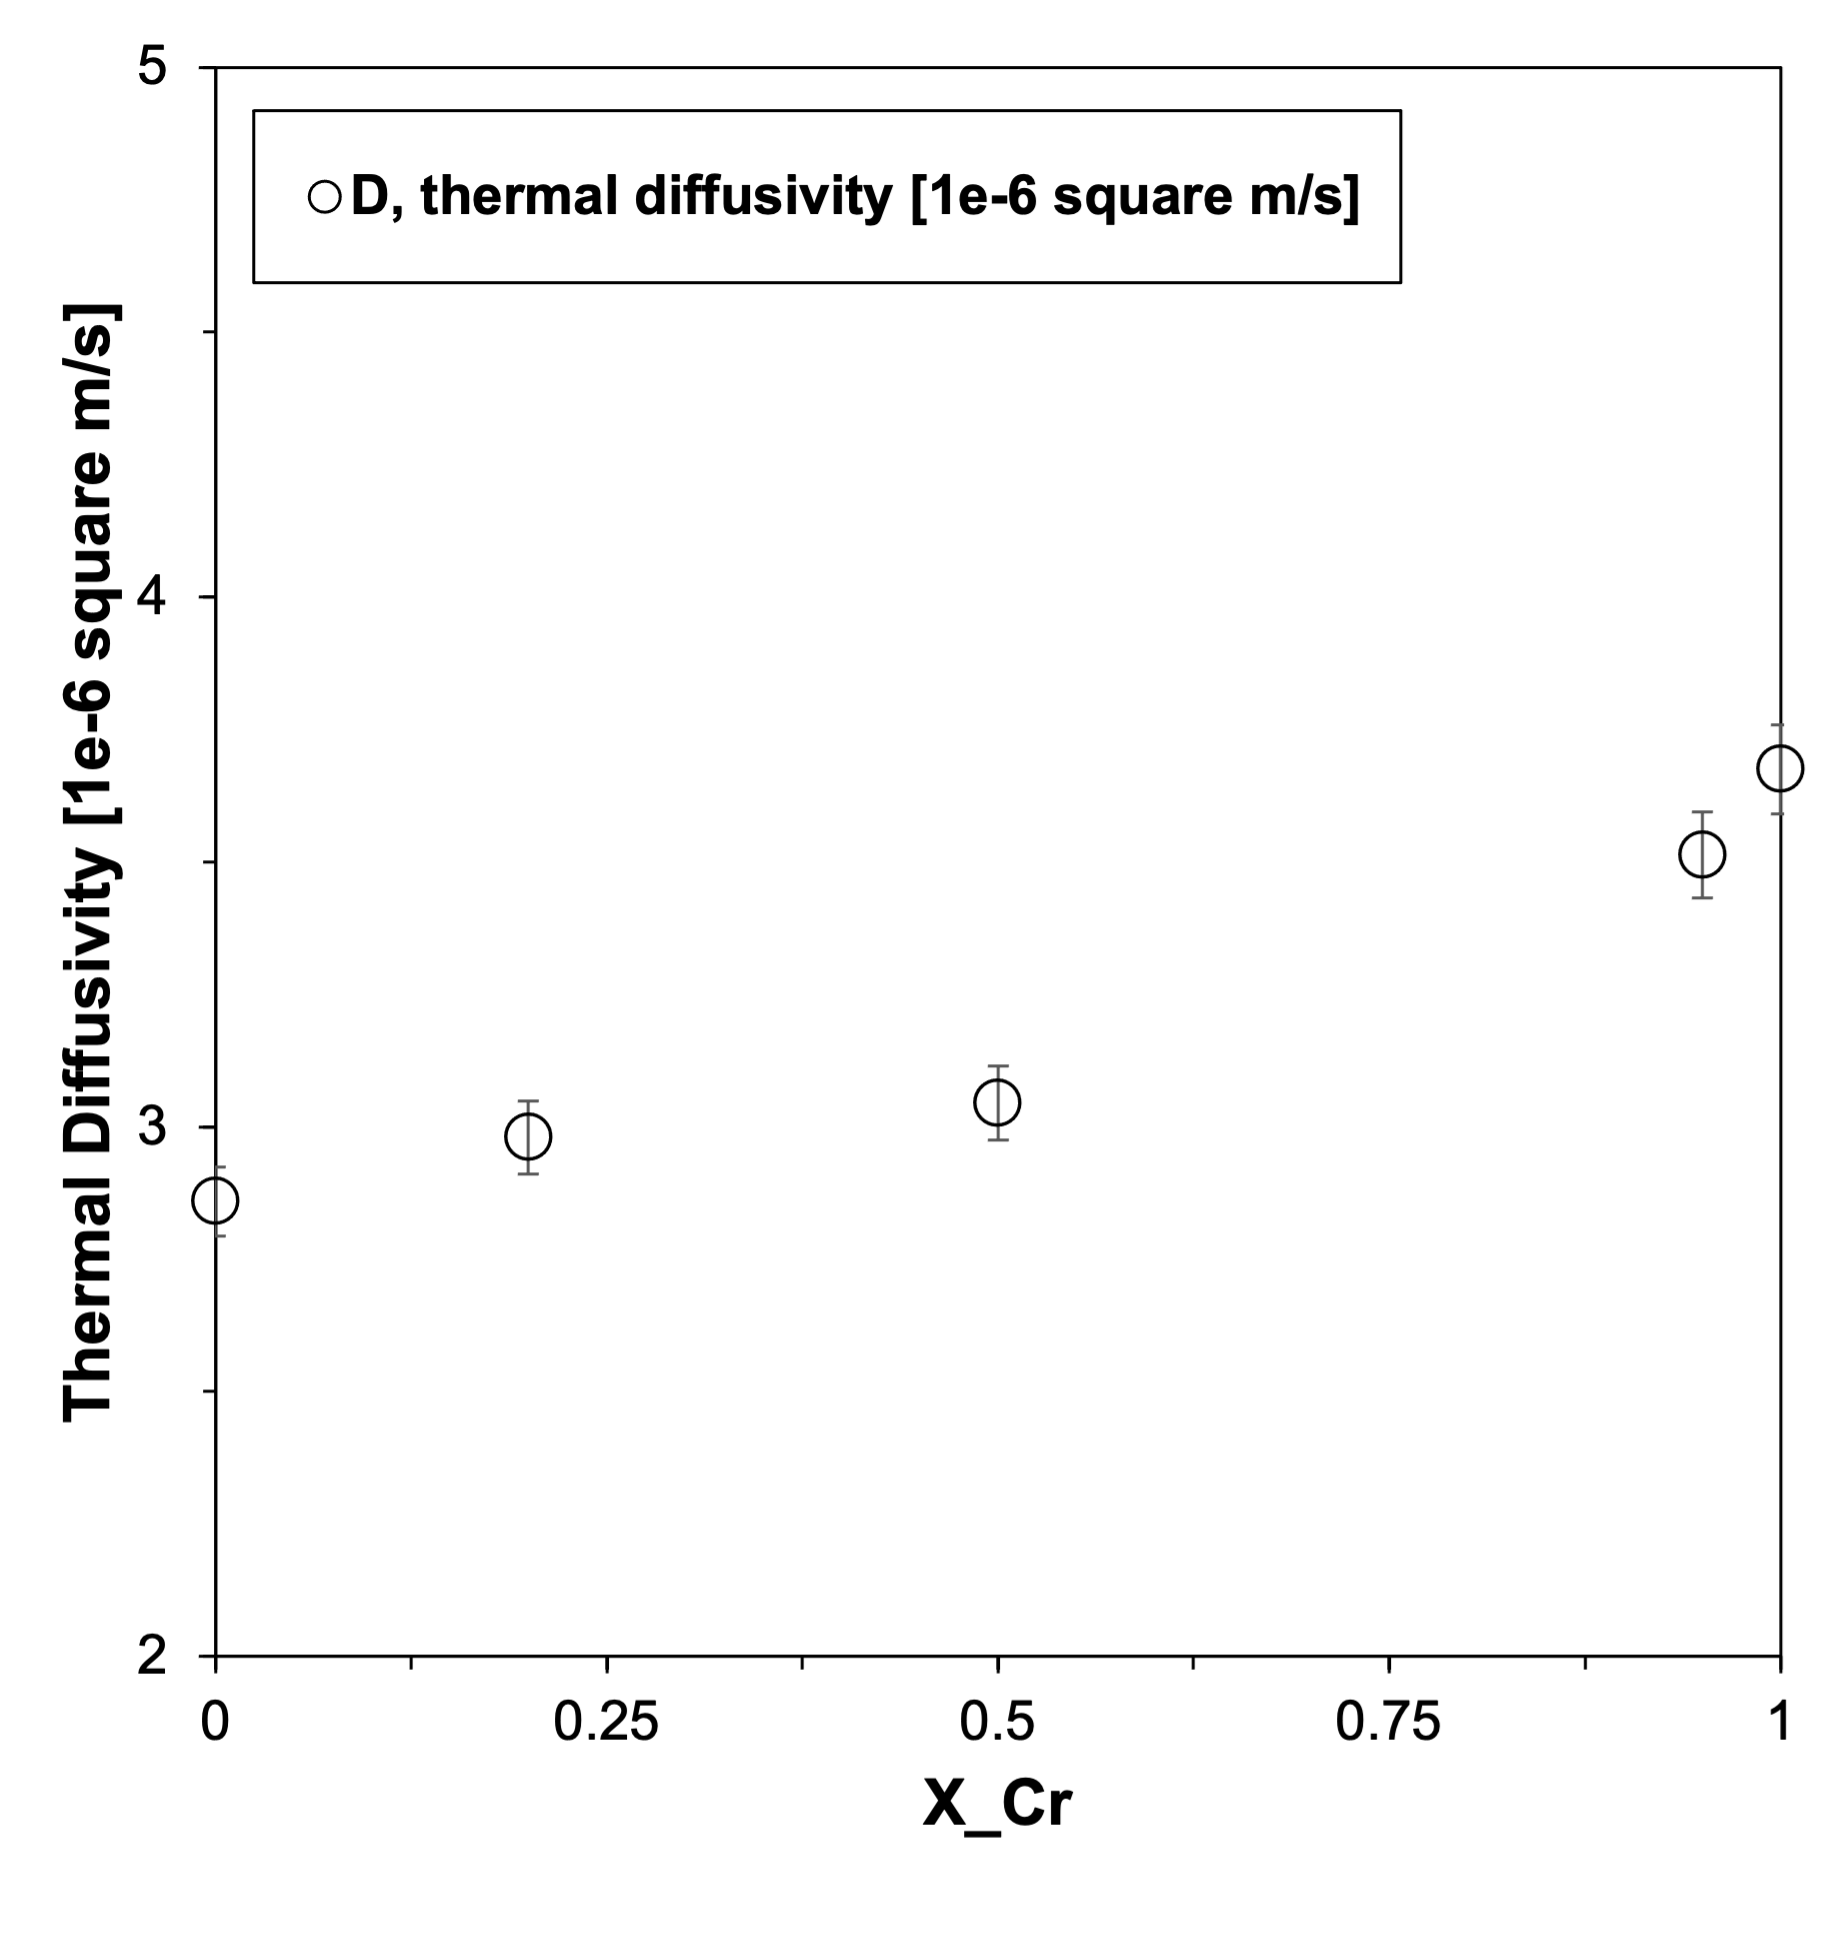
\includegraphics[width=\linewidth]{Parts/Figures/DvsX_v4.png}
         \caption{\(D^{theoretical}_{thermal}\), theoretical thermal diffusivity indicating the expected thermal behavior based on composition and microstructural considerations. This predictive analysis aids in understanding the thermal management potential of the alloy across a range of compositions.}
         \label{fig5e}
     \end{subfigure}
     \hfill
     \begin{subfigure}{0.3\textwidth}
         \centering
         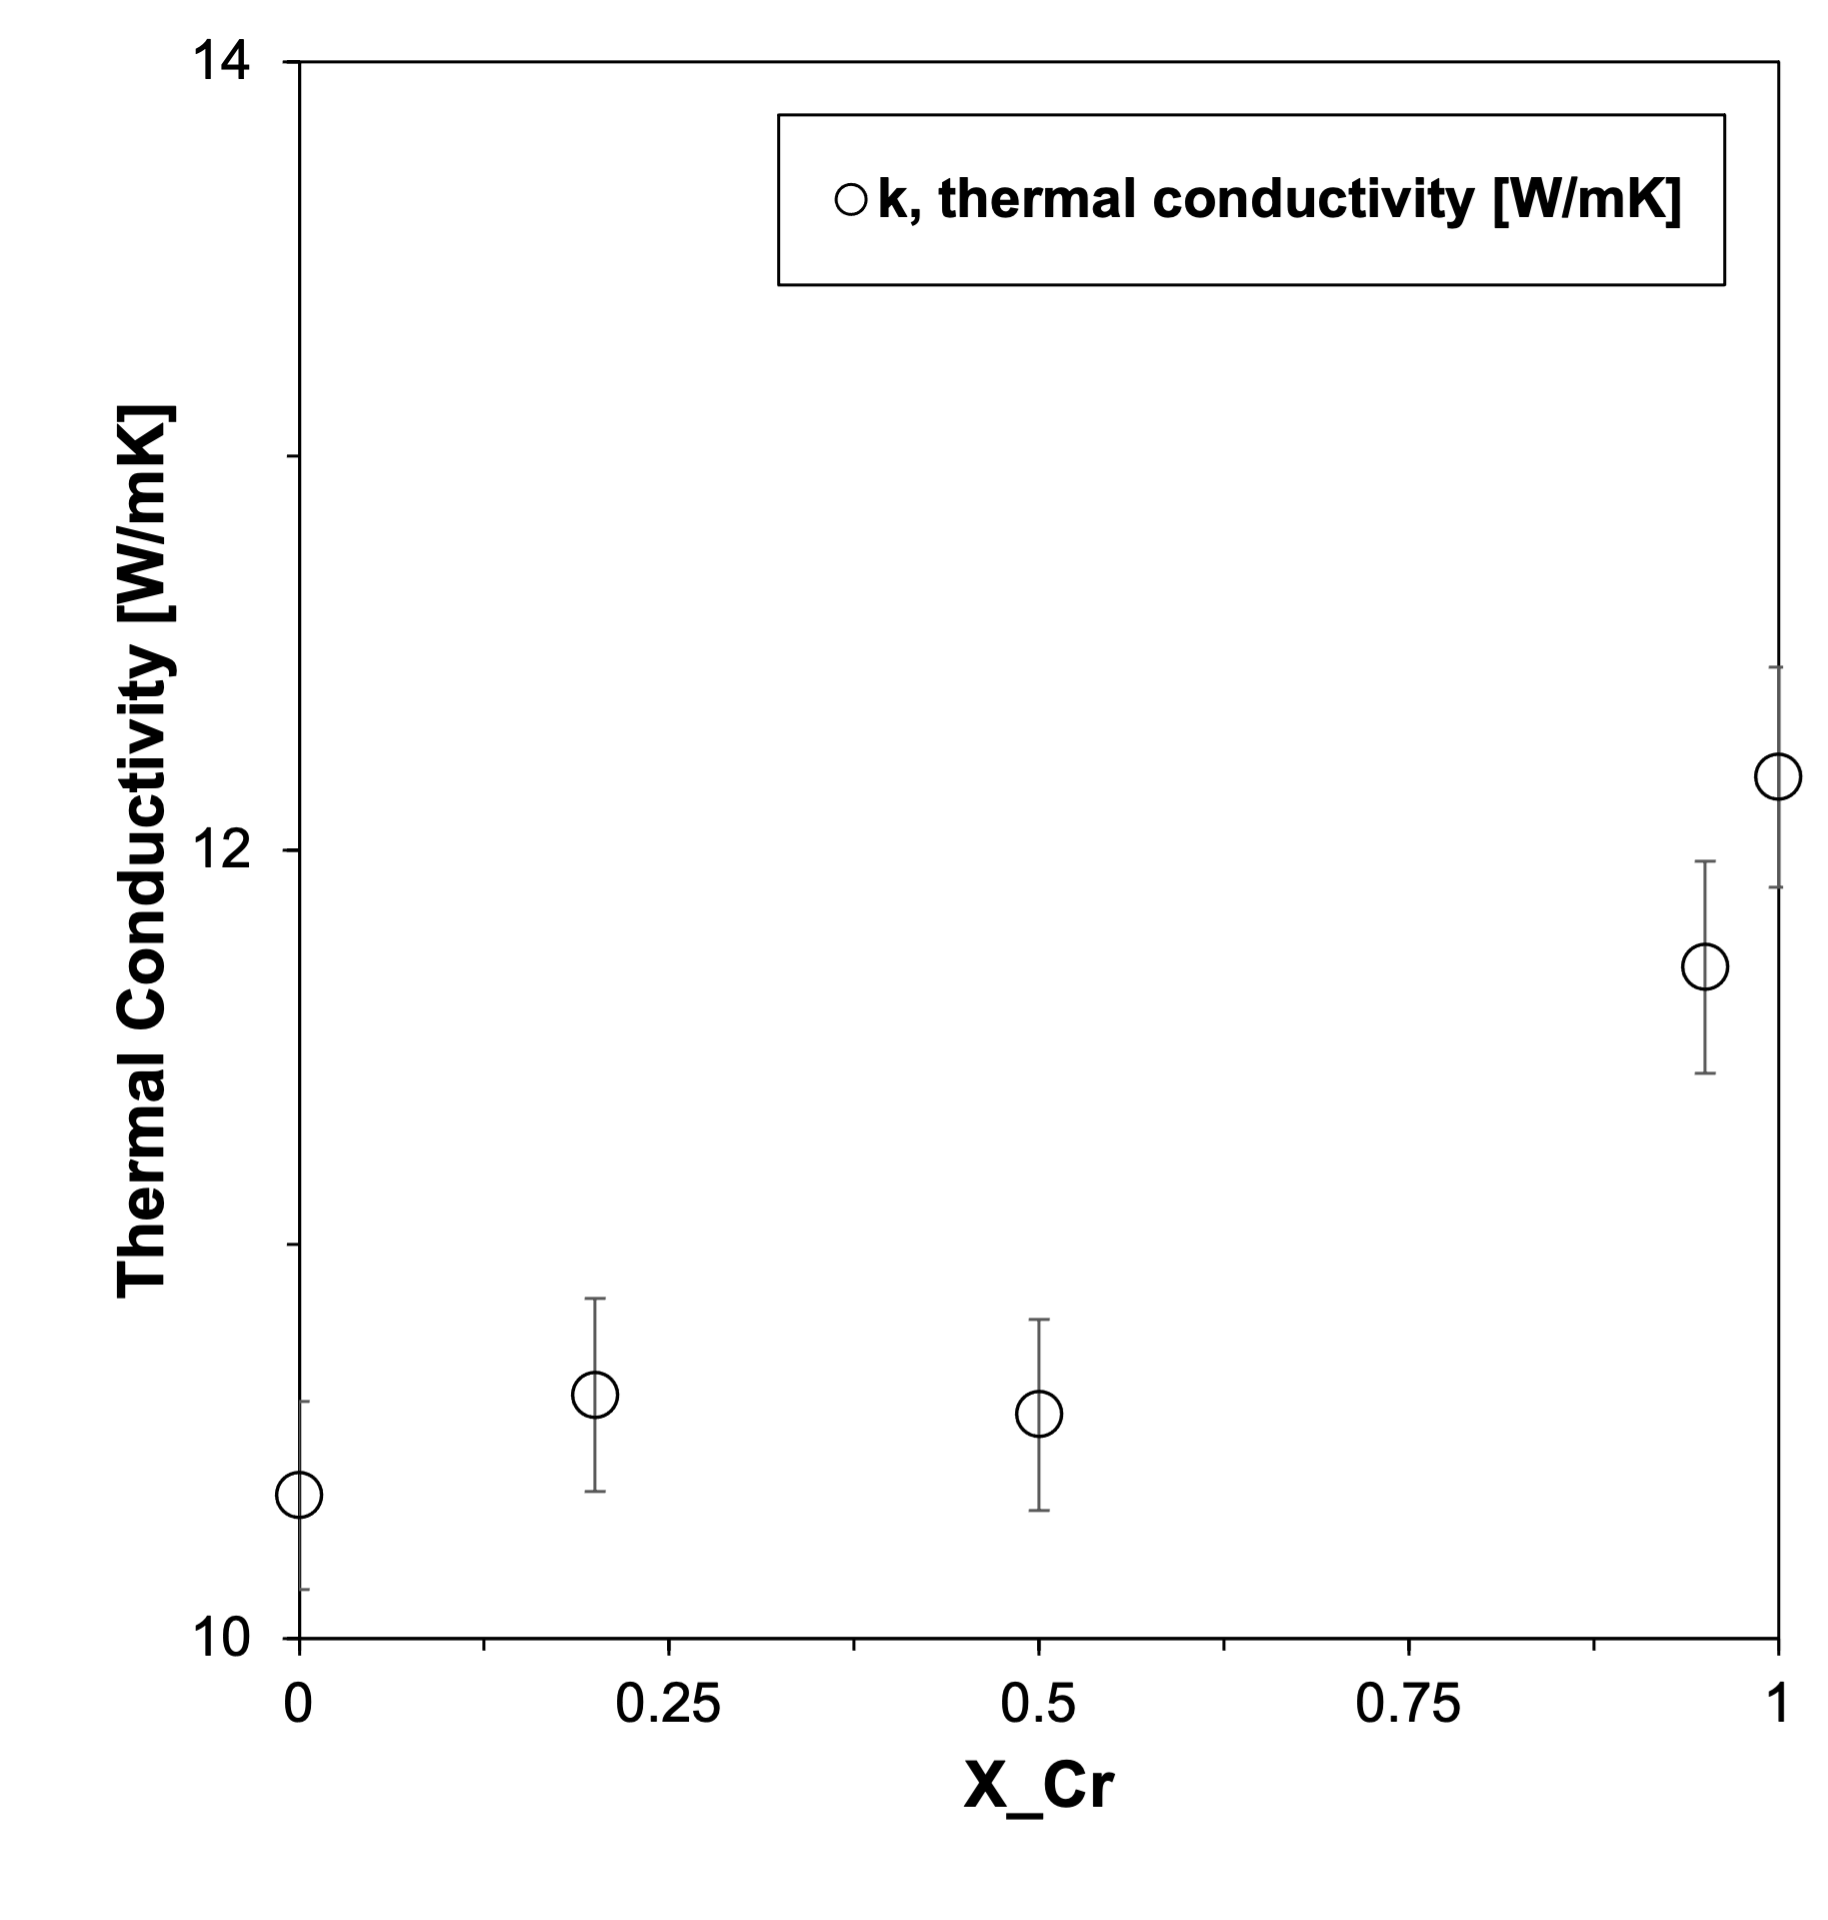
\includegraphics[width=\linewidth]{Parts/Figures/KvsX_v2.png}
         \caption{\(\kappa^{theoretical}_{thermal}\), thermal conductivity, showcasing the theoretical prediction of how efficiently the material conducts heat. This property is crucial for applications where thermal management is key, and it is influenced by the alloy's microstructure and composition.}
         \label{fig5f}
     \end{subfigure}
	\caption{Comprehensive analysis combining experimental and theoretical insights into the thermal and mechanical properties of stainless steels subjected to thermal aging. (a) Experimental elastic moduli trends with aging temperature highlight the stiffening effect of microstructural evolution. (b) and (c) Theoretical predictions for pristine and spinodally decomposed steels provide a comparative framework for assessing the impact of spinodal decomposition on material properties. (d) Experimental thermal diffusivity measurements, alongside (e) theoretical predictions for thermal diffusivity and (f) thermal conductivity, offer a holistic view of the material's thermal and mechanical behavior post-aging, emphasizing the interconnectedness of thermal properties, mechanical performance, and microstructural characteristics.}
	\label{fig5}
\end{sidewaysfigure}


\end{document}
